\newpage
{\bfseries МРНТИ}~52.13.25

{\bfseries ИССЛЕДОВАНИЯ ЗАКОНОМЕРНОСТЕЙ ИЗМЕНЕНИЯ ДЕФОРМАЦИЙ В ЗАВИСИМОСТИ
ОТ ТЕХНОЛОГИЧЕСКИХ ПАРАМЕТРОВ ОЧИСТНОГО ЗАБОЯ ДЛЯ НАКЛОННЫХ ЗАЛЕЖЕЙ}

\textsuperscript{1}Д.К. Таханов, \textsuperscript{1}М.Ж.
Балпанова\textsuperscript{🖂}, \textsuperscript{2}Д.Т. Ивадилинова

\textsuperscript{1}Карагандинский технический университет имени Абылкаса
Сагинова, Караганда, Казахстан

{\bfseries \textsuperscript{🖂}}Корреспондент-автор: balpanova86@mail.ru

В статье рассматривается разработка технологической схемы отработки
наклонных залежей с углом падения от 20 до 35 градусов на примере
Жиландинского месторождения с использованием камерно-столбовой системы.
Ухудшение геомеханических условий, вызванное неправильными параметрами
системы разработки, требует корректировки этих параметров. Для решения
этой проблемы было проведено моделирование массива горных пород с
использованием метода конечных элементов. В результате были определены
главные сжимающие и растягивающие напряжения в зависимости от глубины
отработки. Также был проведен расчет параметров междукамерных целиков с
учетом различных горнотехнических факторов. Анализ результатов
численного моделирования позволил определить допустимые параметры
очистной камеры и междукамерного целика в зависимости от угла залегания.
Было установлено, что междукамерный целик классической вертикальной
формы допустим только при угле падения рудного тела до 25 градусов.
Новая технология отработки наклонных залежей с углом падения 20-35
градусов с использованием камерно-столбовой системы была разработана на
основе исследований Жиландинского месторождения.

Ключевые слова: наклонная залежь, междукамерный целик, устойчивость,
очистная камера, запас прочности, численное моделирование, система
разработки.

КӨЛБЕУ КЕН ОРЫНДАРЫ ҮШІН ТАЗАРТУ КЕНЖАРЫНЫҢ ТЕХНОЛОГИЯЛЫҚ ПАРАМЕТРЛЕРІНЕ
БАЙЛАНЫСТЫ ДЕФОРМАЦИЯЛАРДЫҢ ӨЗГЕРУ ЗАҢДЫЛЫҚТАРЫН ЗЕРТТЕУ

\textsuperscript{1}Д.К. Таханов, \textsuperscript{1}М.Ж.
Балпанова\textsuperscript{🖂}, \textsuperscript{1}Д.Т. Ивадилинова

\textsuperscript{1}Әбілқас Сағынов атындағы Қарағанды техникалық
университеті, Қарағанды, Қазақстан

е-mail: balpanova86@mail.ru

Мақалада камералық-бағаналы қазу жүйесін қолдана отырып, Жыланды кен
орнының мысалында құлау бұрышы 20-дан 35 градусқа дейінгі көлбеу
кеншоғырларды өндірудің технологиялық схемасын әзірлеу қарастырылды.
Қазу жүйесінің теріс қабылданған параметрлерінен туындаған
геомеханикалық жағдайлардың нашарлауы осы параметрлерді түзетуді қажет
етеді. Бұл мәселені шешу үшін соңғы элементтер әдісін қолдана отырып,
тау жыныстарының массивін модельдеу жүргізілді. Нәтижесінде жұмыс
тереңдігіне байланысты негізгі қысу және созылу кернеулері анықталды.
Сондай-ақ, әртүрлі тау-кен факторларын ескере отырып, камерааралық
кентіректердің параметрлерін есептеу жүргізілді. Сандық модельдеу
нәтижелерін талдау тазарту камерасы мен камерааралық кентіректердің
рұқсат етілген параметрлерін еңіс бұрышына байланысты анықтауға
мүмкіндік берді. Классикалық тік форманың камерааралық кентірек кен
денесінің 25 градусқа дейін еңіс бұрышында ғана рұқсат етілетіні
анықталды. Камералық-бағаналы қазу жүйесін пайдалана отырып, 20-35
градус құлау бұрышы бар көлбеу кеншоғырларды өндірудің жаңа технологиясы
Жыланды кен орнын зерттеу негізінде әзірленді.

Түйін сөздер: көлбеу кеншоғыр, камерааралық кентірек, тұрақтылық,
тазарту камерасы, беріктік қоры, сандық модельдеу, қазу жүйесі.

STUDIES OF THE PATTERNS OF DEFORMATION CHANGES DEPENDING ON THE
TECHNOLOGICAL PARAMETERS OF THE TREATMENT FACE FOR INCLINED DEPOSITS

\textsuperscript{1}D.K. Takhanov, \textsuperscript{1}M.J.
Balpanova\textsuperscript{🖂}, D.T. Ivadilinova\textsuperscript{1}

\textsuperscript{1} Karaganda Technical University named after Abylkas
Saginov, Karaganda, Kazakhstan

е-mail: balpanova86@mail.ru

The article considers the development of a technological scheme for
mining inclined deposits with an angle of incidence from 20 to 35
degrees on the example of the Zhilandy deposit using a chamber-column
system. Deterioration of geomechanical conditions caused by incorrect
parameters of the development system requires adjustment of these
parameters. To solve this problem, modeling of the rock mass using the
finite element method was carried out. As a result, the main compressive
and tensile stresses were determined depending on the depth of working.
The calculation of the parameters of the inter-chamber targets was also
carried out taking into account various mining factors. The analysis of
the numerical simulation results made it possible to determine the
permissible parameters of the cleaning chamber and the inter-chamber
whole depending on the angle of occurrence. It was found that the
inter-chamber whole of the classical vertical shape is permissible only
when the angle of incidence of the ore body is up to 25 degrees. A new
technology for mining inclined deposits with an angle of incidence of
20-35 degrees using a chamber-column system was developed based on
studies of the Zhilandy deposit.

Keywords:~inclined deposit, inter-chamber whole, stability, cleaning
chamber, safety margin, numerical modeling, development system

{\bfseries Введение.} Технологические параметры очистного забоя при
камерно-столбовой системе разработки зависит от формы и расположения
междукамерных целиков.

Расчет параметров барьерных и междукамерных целиков осуществляется с
учетом следующих горнотехнических условий разработки: глубины
разработки, мощности и угла падения рудной залежи, сложности
горно-геологических условий разработки, физико-механических свойств
пород (прочность, крепость), трещиноватости и строения вмещающих пород.

Для решения тех или иных инженерных задач горного дела, помимо
качественного описания геомеханических процессов, необходима их
количественная оценка, которая может быть получена в результате натурных
измерений различных проявлений геомеханических процессов или в
результате их моделирования. Моделирование обладает тем преимуществом по
сравнению с натурными измерениями, что раскрывает общие качественные и
количественные закономерности геомеханических процессов. Для анализа
геомеханических процессов зачастую используется математическое
моделирование.

В инженерной практике для учета факторов, которые не удается ввести в
расчетную схему, используют различные коэффициенты, полученные
эмпирическим путем на основе натурных наблюдений или данных лабораторных
испытаний. Такой подход чреват эффектом «накопления ошибок»:
проектировщик выбирает значение нужных ему коэффициентов из некоторого
диапазона, не имея достаточного основания для выбора именно этих
значений. Чем больше коэффициентов нужно ввести, тем больше вероятность
того, что получаемая в результате величина отклоняется от своего
истинного значения, и тем больше это отклонение. С развитием новых
вычислительных технологий в горном деле численные методы стали все более
популярными в математическом моделировании для решения различных
инженерных задач. Они дополняют традиционные аналитические методы.

Более точное решение поставленной задачи можно получить, если расчетная
схема и метод решения позволяют изначально учесть интересующие
исследователя факторы. Широкие возможности открывают в этом плане так
называемые численные методы решения, заимствованные из механики
деформируемого твердого тела. Наиболее эффективные из них -- метод
конечных элементов (МКЭ) и метод граничных элементов (МГЭ). Интенсивное
их развитие и применение в практике инженерных расчетов стало возможным
с развитием и доступностью вычислительной техники.

Одним из широко используемых в решении задач горного дела методами
конечных элементов является программа RS-2, разработанный компанией
Rocscience. Программное обеспечение RS-2 предназначена для двухмерного
анализа массива горных пород методами конечных элементов. Программа
позволяет моделировать и анализировать сложные геотехнические задачи.

{\bfseries Материалы и методы.} Решение задач механики деформируемого
твердого тела методом конечных элементов основывается на применении
приближенных методов вычислений, методов матричной и линейной алгебры.
Численное моделирование массива горных пород методам конечных элементов
в ПО RS-2 позволяет определить зоны разгрузки и концентрации напряжения,
смещения пород, коэффициент запаса прочности, величину главных
напряжений действующие в массиве, зоны упругих и неупругих деформации и
величины коэффициента запаса прочности пород, расчет параметров крепи и
многих других процессов, происходящие вокруг выработанного пространства.

Данные о характеристиках горных пород и руд получены с результатов,
ранее выполненных исследовании на Жыландинской группы месторождения
{[}1{]}. В таблице 1 приведены физико-механические свойства и данные о
структурных свойствах массива горных пород для выполнения численного
моделирования массива горных пород с использованием по RS-2.

Целью моделирования является определение допустимых параметров очистной
камеры и междукамерных целиков при отработке наклонных залежей углом
падения до 35 градусов.

{\bfseries Таблица 1 -- Деформационно-прочностные характеристики образцов
горных пород проб 1-5 в водонасыщенном состоянии при одноосном сжатии}

\begin{figure}[H]
	\centering
	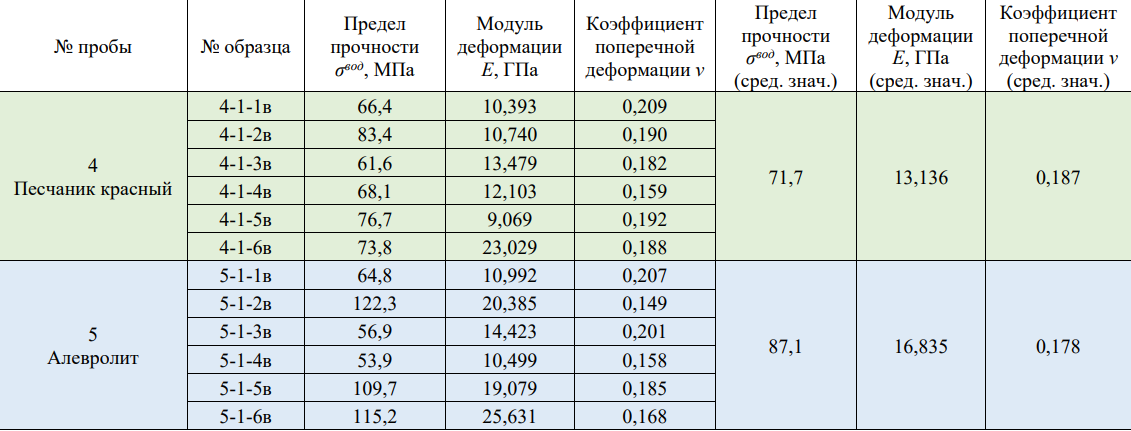
\includegraphics[width=0.8\textwidth]{assets/281}
	\caption*{}
\end{figure}

При моделировании эти значения были обобщены, изменялся лишь параметр
GSI. Рейтинг GSI является одним из важных параметров, существенно
влияющих на результаты моделирование. В расчетах выполнялись с
применением критерия Хука-Брауна. GSI, представленный Хуком и Брауном в
1994, 1995 и 1998 г.г., представляет собой систему полевого определения
прочности породного массива для различных геологических условий, которая
основана на визуальной оценке структуры массива (блочности) и
характеристик трещин (шероховатость и степень изменения). Сочетание этих
двух параметров позволяет выполнить оценку породного массива, имеющего
различную структуру.

Для обоснования параметров очистной камеры и целиков выполнялся
численное моделирование с изменением ширины камер и МКЦ. Моделирование
выполнялось для углов падение 20, 25, 30 и 35 градусов. В ходе
моделирование определены показатели коэффициента запаса прочности (SF),
а также показатели главных сжимающих (Sigma1) и растягивающих (Sigma3)
напряжений. Определение необходимых участков, таких как зона
концентрации и разгрузки напряжения, осуществляется за счет главных
сжимающих и растягивающих напряжений {[}2{]}.

При проведении горной выработки происходит перераспределение напряжений
в окружающих породах: одни из компонентов тензора напряжений возрастают,
другие уменьшаются. Степень изменения напряжений по сравнению с исходным
их уровнем называется концентрацией и разгрузкой. По стандаратам
международного общества по горной механике (ISRM) для безопасного
ведения горных работ, коэффициент запаса устойчивости горных пород
должен быть выше значение 1,2 {[}3{]}.

Значение 1,2, использованное в рамках исследования, принято на основании
исследования Рида и Стэйси (2009 г.), проведенного в продолжение работ
Суона и Сепульведы (2000 г.). результаты данных исследовании признана
международным обществом по горной механике (ISRM) {[}3{]}.

Для горнотехнических условий разработки Жиландинского месторождения
расположение междукамерных целиков принимается по квадратной сетке с
расстоянием между осями равным 20х20м.

Согласно Технологическому регламенту по применению камерно-столбовой
системы разработки с оставлением столбчатых целиков на подземных
рудниках Жезказганского месторождения {[}4{]}, при отработке наклонных
залежей соблюдать следующие условия расположения междукамерных целиков:

- в диапазоне изменения углов падения залежей 15˚-25˚ междукамерные
целики размещать вертикально;

- в диапазоне изменения углов падения залежей свыше 25˚ до 35˚
междукамерные целики должны быть размещены с наклоном в сторону
восстания на угол β = α/2 (где: α -- угол падения залежей) относительно
нормали к напластованию.

{\bfseries Результаты и обсуждения}. На ниже приведенных рисунках
представлены результаты численного моделирования при мощности рудного
тела 5 метров и при углах падения 20-35 градусов. Моделирование
выполнено на основе анализа физико-механических свойств и структурных
особенностей горных пород.

\begin{figure}[H]
	\centering
	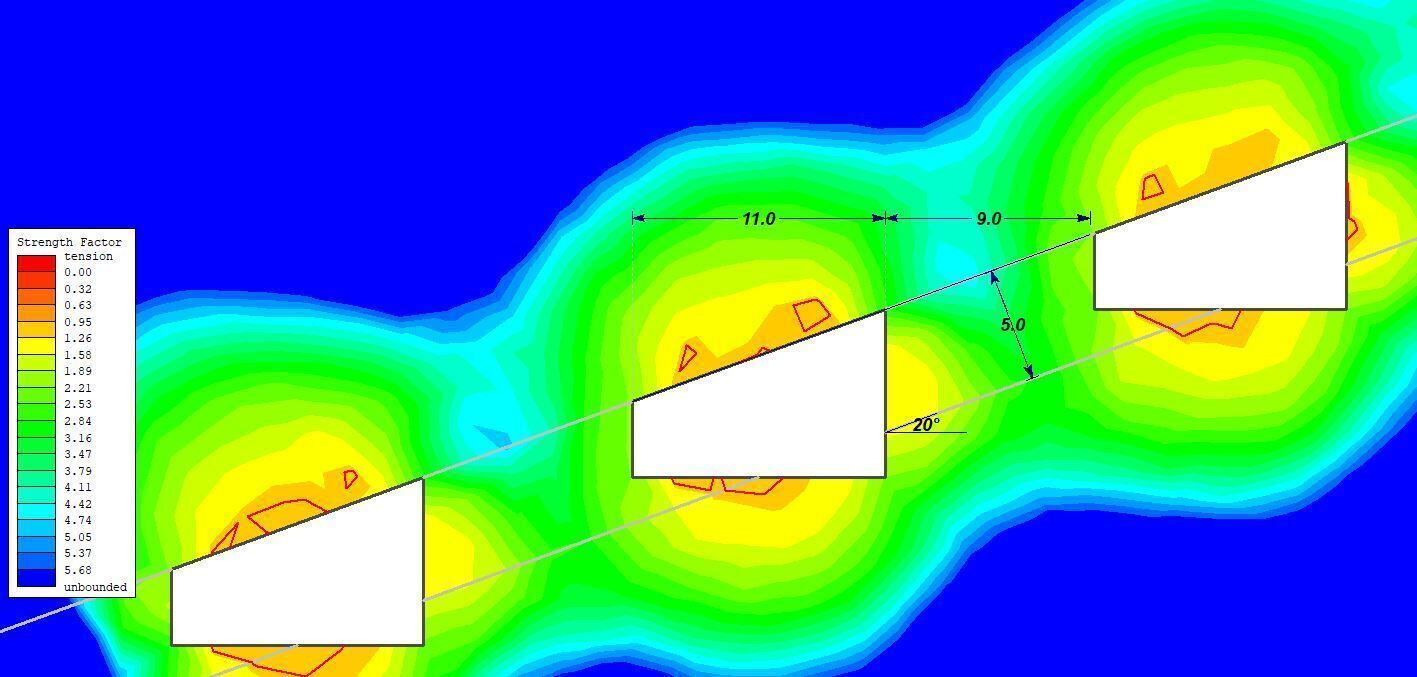
\includegraphics[width=0.8\textwidth]{assets/282}
	\caption*{}
\end{figure}

{\bfseries Рис. 1 -- Коэффициент запаса прочности законтурного массива при
параметрах очистной камеры 11х9 м и при угле падения 20 градусов}

\begin{figure}[H]
	\centering
	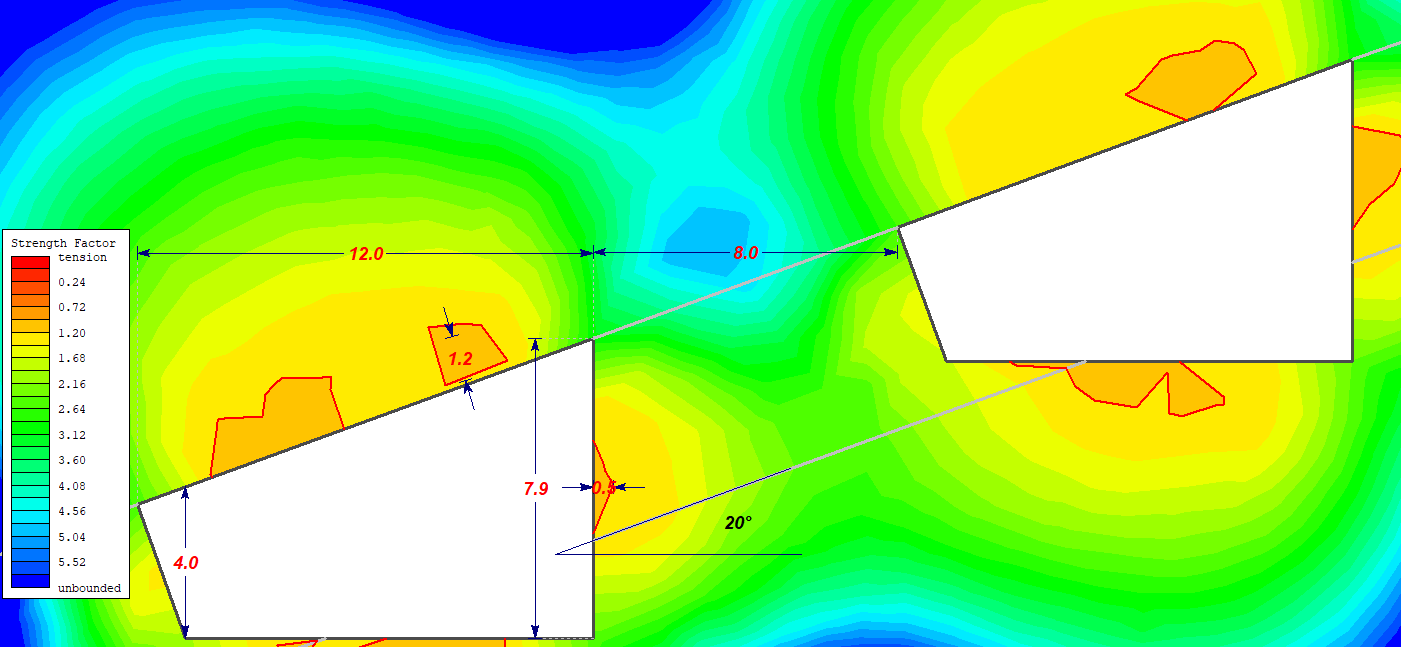
\includegraphics[width=0.8\textwidth]{assets/283}
	\caption*{}
\end{figure}

{\bfseries Рис. 2 -- Коэффициент запаса прочности законтурного массива при
параметрах очистной камеры 12х8 м и при угле падения 20 градусов}

\begin{figure}[H]
	\centering
	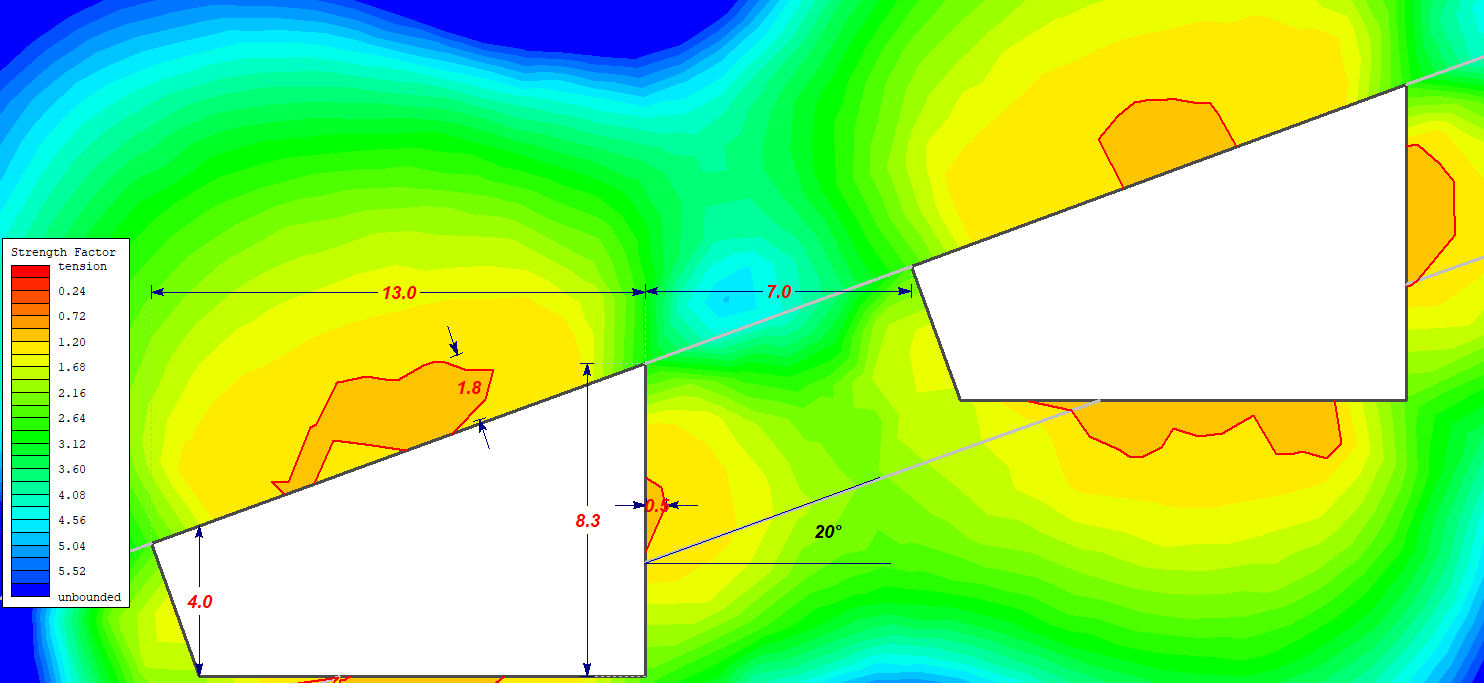
\includegraphics[width=0.8\textwidth]{assets/284}
	\caption*{}
\end{figure}

{\bfseries Рис. 3 -- Коэффициент запаса прочности законтурного массива при
параметрах очистной камеры 13х7 м и при угле падения 20 градусов}

\begin{figure}[H]
	\centering
	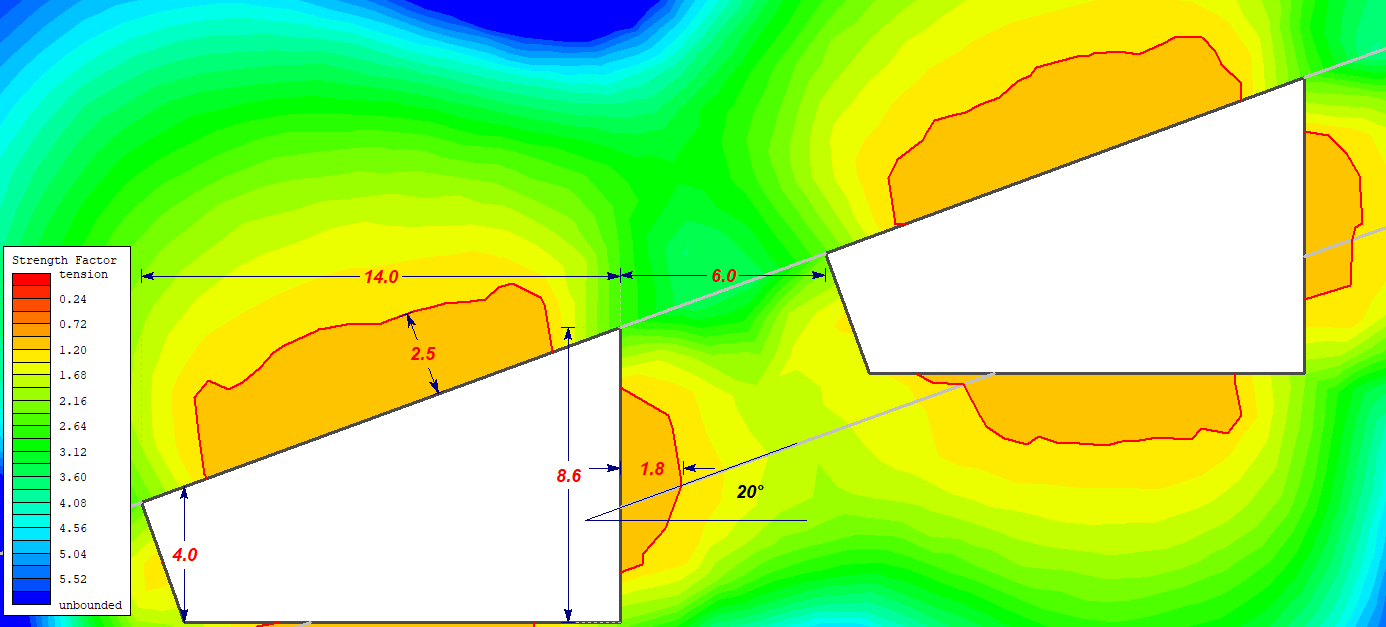
\includegraphics[width=0.8\textwidth]{assets/285}
	\caption*{}
\end{figure}\textbackslash{}

{\bfseries Рис. 4 -- Коэффициент запаса прочности законтурного массива при
параметрах очистной камеры 14х6 м и при угле падения 20 градусов}

По результатам моделирования, представленные на рисунках 1, 2 и 3 видно,
что при угле падения 20 градусов очистная камера и целики в целом
находятся в устойчивом состоянии. К чему свидетельствует запас прочности
массива горных пород, представленного виде графика на рисунке 5. По
графику видно, что минимальный запас прочности выше значение 1.2, из
которого следует предполагать, что МКЦ и очистная камера находится в
устойчивом состояний. Максимально допустимая ширина очистной камеры
равен 13.0 метров при минимальной мощности МКЦ 7.0 метров.

При ширине камеры 14 метров и мощности МКЦ 6 метров (рис. 4) высота
неустойчивых участков по кровле камеры составляет 2,5 метров, а
разрушение МКЦ достигает до 1,8 метров, из чего следует утверждать, что
риски обрушения горных пород и разрушения МКЦ велики.

При отработке запасов руды при угле падения 20 градусов
камерно-столбовой системой разработки законтурный массив устойчив,
возможны локальные разрушения горных пород до 0,5 метров преимущественно
с кровли выработки виде отслоений и заколов {[}5{]}. МКЦ находится в
устойчивом состояний, к чему свидетельствует запас прочности МКЦ 1,3 и
более.

При отработке запасов руды при угле падения 20 градусов не требуется
изменение формы МКЦ на трапециевидную, так как прямые столбчатые МКЦ в
полной мере могут обеспечить устойчивость массива горных пород.

{\bfseries Рис. 5 -- Изменение коэффициента запаса прочности МКЦ в
зависимости от изменения ширины камеры и мощности МКЦ}

Далее был выполнен моделирование с изменением угла падения до 25
градусов результаты которого приведены на рисунках 6 и 7.

\begin{figure}[H]
	\centering
	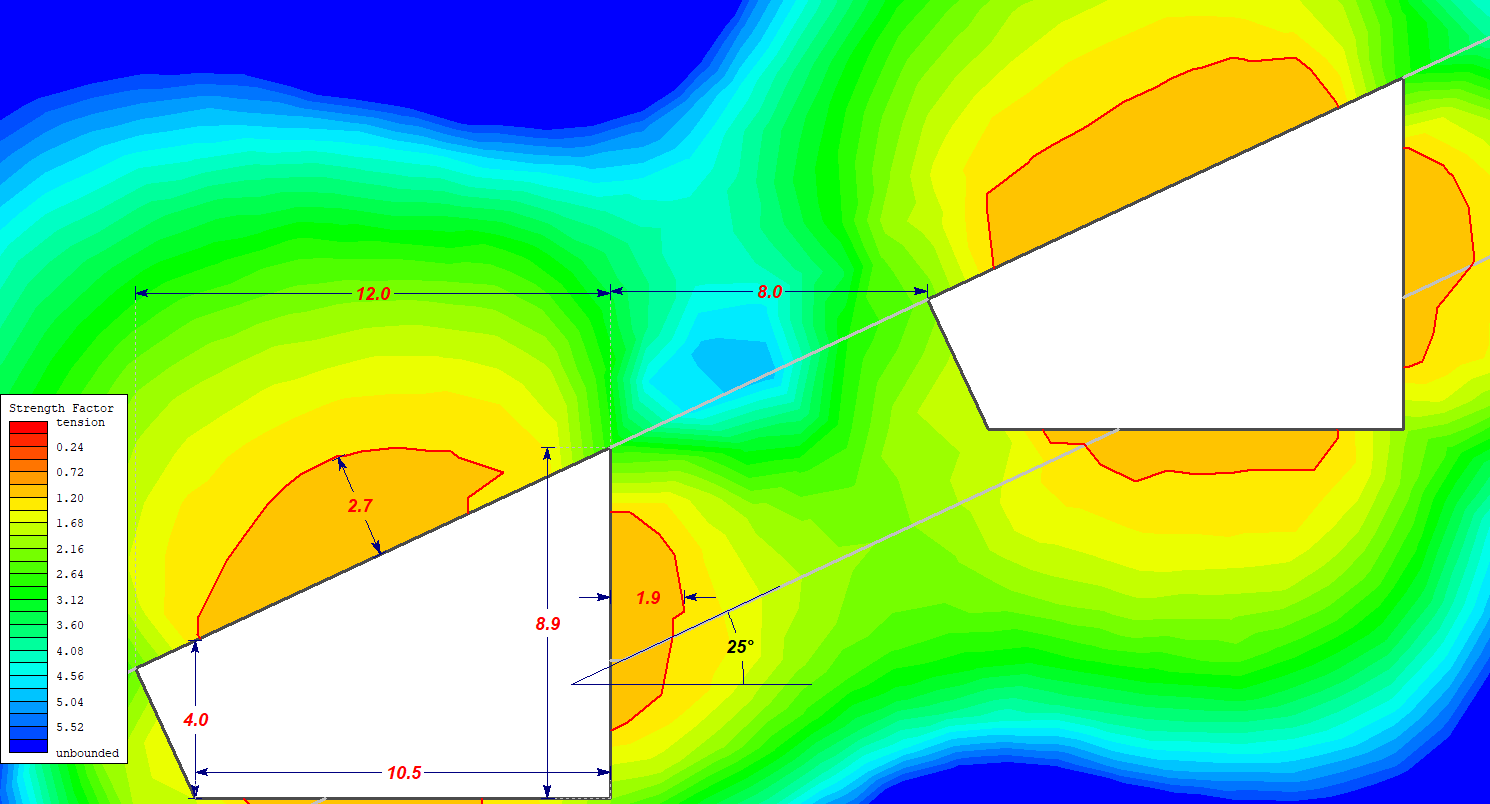
\includegraphics[width=0.8\textwidth]{assets/286}
	\caption*{}
\end{figure}

{\bfseries Рис. 6 -- Коэффициент запаса прочности законтурного массива при
параметрах очистной камеры 12х8 м и при угле падения 25 градусов}

По результатам численного анализа (рис. 6) видно, что при ширине камеры
12 метров и диаметре МКЦ 8 метров коэффициент запаса прочности пород
находятся выше критической отметки равной 1.2. Также результаты
моделирования показал, что возможны обрушения части МКЦ до глубины 1,9
метра, а по кровле очистной камеры зона возможного обрушения доходит до
2,7 метра. В целом МКЦ и очистная камера находится в устойчивом
состоянии.

\begin{figure}[H]
	\centering
	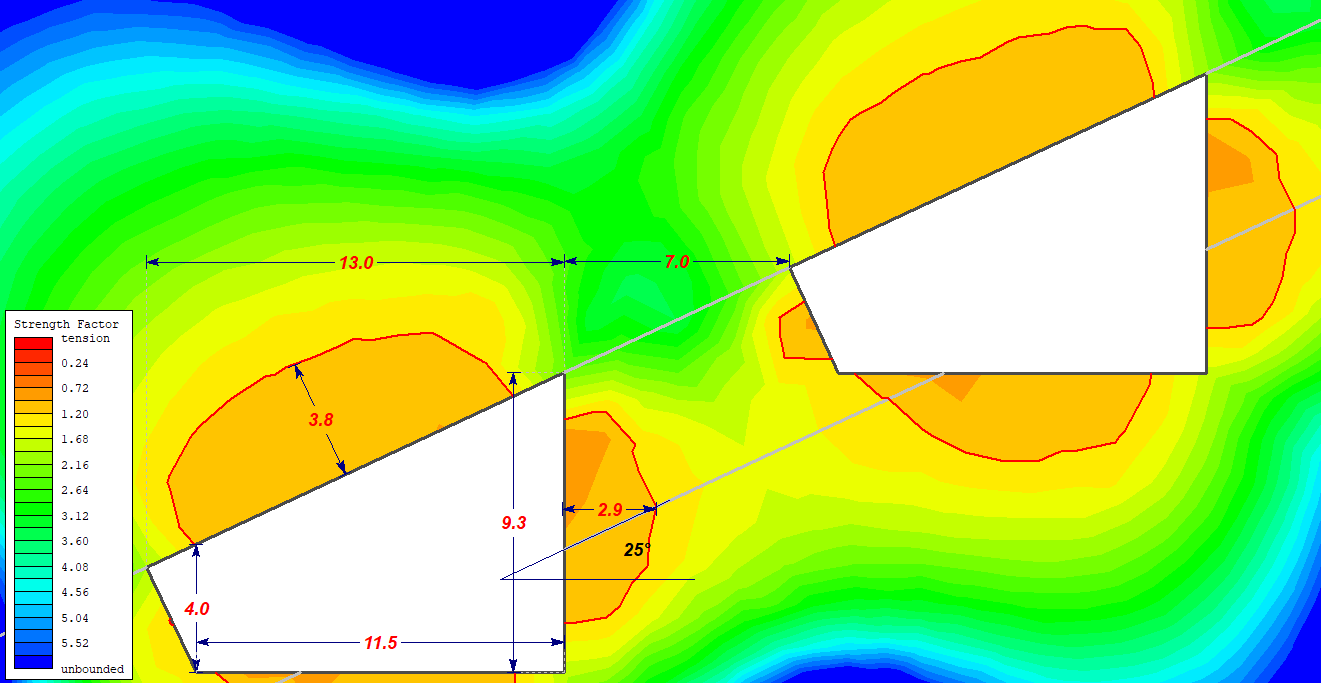
\includegraphics[width=0.8\textwidth]{assets/287}
	\caption*{}
\end{figure}

{\bfseries Рис. 7 -- Коэффициент запаса прочности законтурного массива при
параметрах очистной камеры 13х7 м и при угле падения 25 градусов}

На рисунке 7 приведены результаты численного анализа при ширине камеры
13 метров и диаметре МКЦ 7 метров. При таких параметрах по кровле
очистной камеры возможны обрушения до глубины 3,8 метров, а разрушение
МКЦ может достигать до 2,9 метров.

На рисунке 8 приведены изменение коэффициента запаса прочности МКЦ в
зависимости отдаленности от контура камеры.

При угле 25 градусов был выбран трапециевидная форма МКЦ, так как
результаты численного анализа показали, что при столбчатой форме МКЦ
вероятность разрушение МКЦ более высокая. Сравнение результатов
моделирования запаса прочности трапециевидной и прямоугольной МКЦ
диаметром 8 метров приведен на рисунке 9.

Исходя из вышеизложенного следует, что классическая (прямоугольная)
форма МКЦ не эффективен при угле падения рудного тела 25 градусов и
более. Следовательно, при численном анализе массива горных пород при
углах падения рудного тела 30-35 градусов целесообразно принимать
трапециевидную форму МКЦ.

\begin{figure}[H]
	\centering
	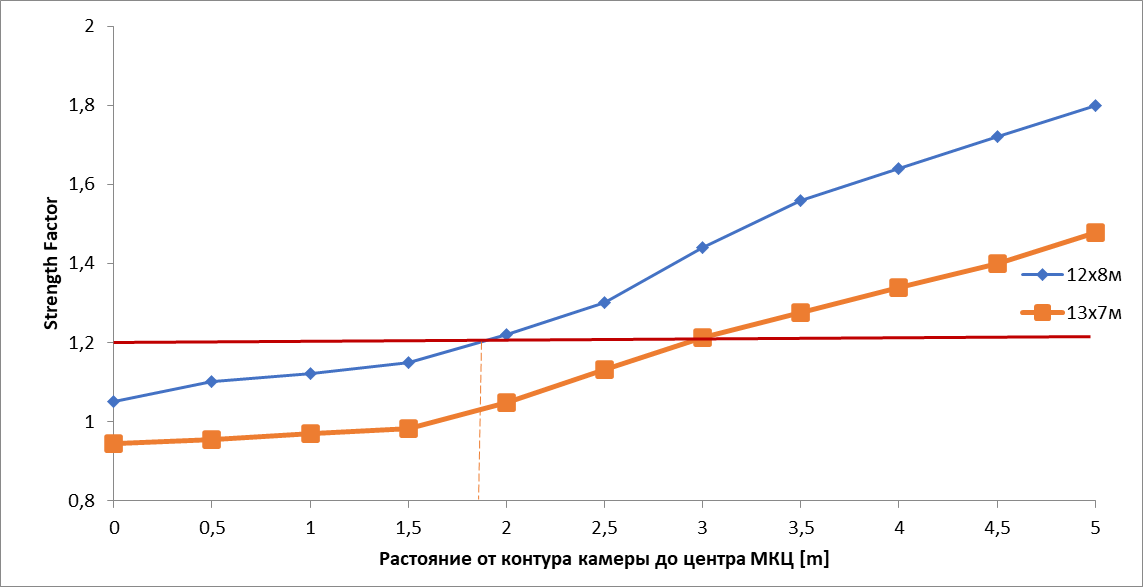
\includegraphics[width=0.8\textwidth]{assets/288}
	\caption*{}
\end{figure}

{\bfseries Рис. 8 -- Изменение коэффициента запаса прочности МКЦ}

\begin{figure}[H]
	\centering
	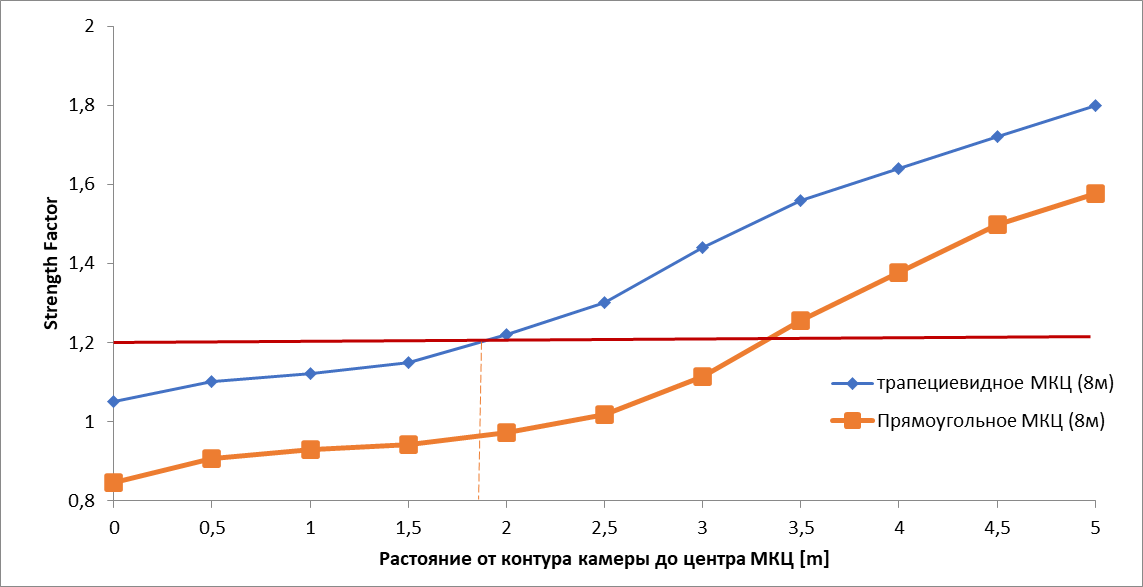
\includegraphics[width=0.8\textwidth]{assets/289}
	\caption*{}
\end{figure}

{\bfseries Рис. 9 -- Сравнение трапециевидной и прямоугольной формы МКЦ}

На рисунках 10-11 представлены результаты моделирования при угле 30
градусов. Следует отметить, что при ширине камеры 12 метров и диаметре
МКЦ 8 метров. При таких параметрах по кровле очистной камеры возможны
обрушения до глубины 4,6 метров, а разрушение МКЦ может достигать до 5,3
метров (рис. 10).

\begin{figure}[H]
	\centering
	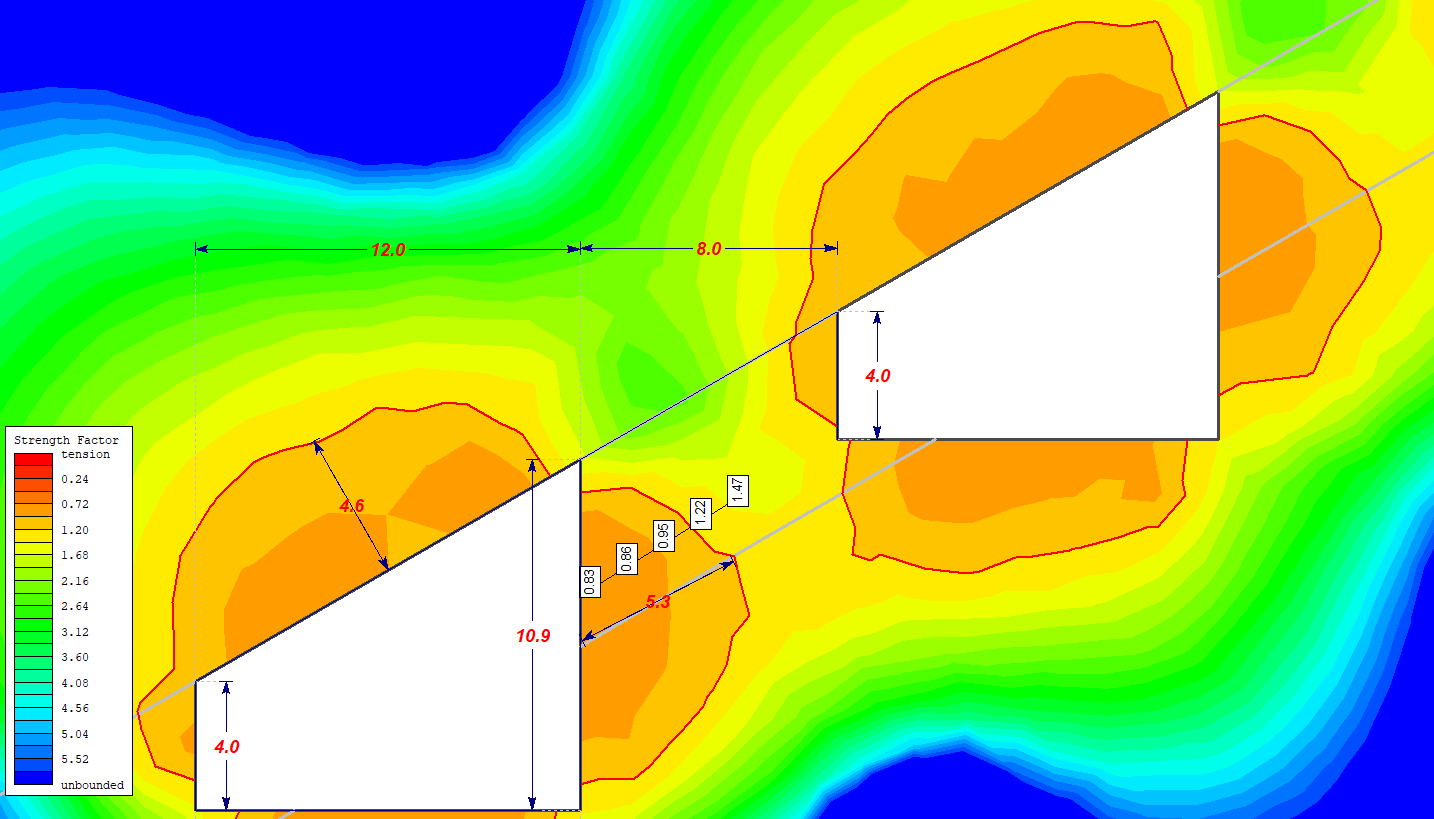
\includegraphics[width=0.8\textwidth]{assets/290}
	\caption*{}
\end{figure}

{\bfseries Рис. 10 -- Коэффициент запаса прочности законтурного массива при
параметрах очистной камеры 12х8 м и при угле падения 30 градусов}

Далее был выполнен численный анализ с изменением формы МКЦ и очистной
камеры на трапециевидную форму {[}6{]}.

Аналогично как на предыдущих моделях был выполнен численный анализ с
изменением ширины камеры на 11 метров, соответственно диаметра МКЦ на 9
метров. На рисунке 11 приведены результаты численного моделирования. По
рисунку видно, что зона возможного обрушения по кровле очистной камеры
не превышает 1,9 метров, тогда как, разрушение МКЦ не превышает 1,8
метра, коэффициент запаса прочности пород больше отметки 1.2, что
говорит об устойчивости МКЦ и камеры.

На рисунке 12 представлена график изменение запасов прочности
классической (12х8 м) и трапециевидной (11х9 м) формы МКЦ, по которому
следует, что при классической форме возможная глубина разрушения может
достигать более 5 метров, тогда как при трапециевидном МКЦ данный
показатель не более 1,8 метров.

\begin{figure}[H]
	\centering
	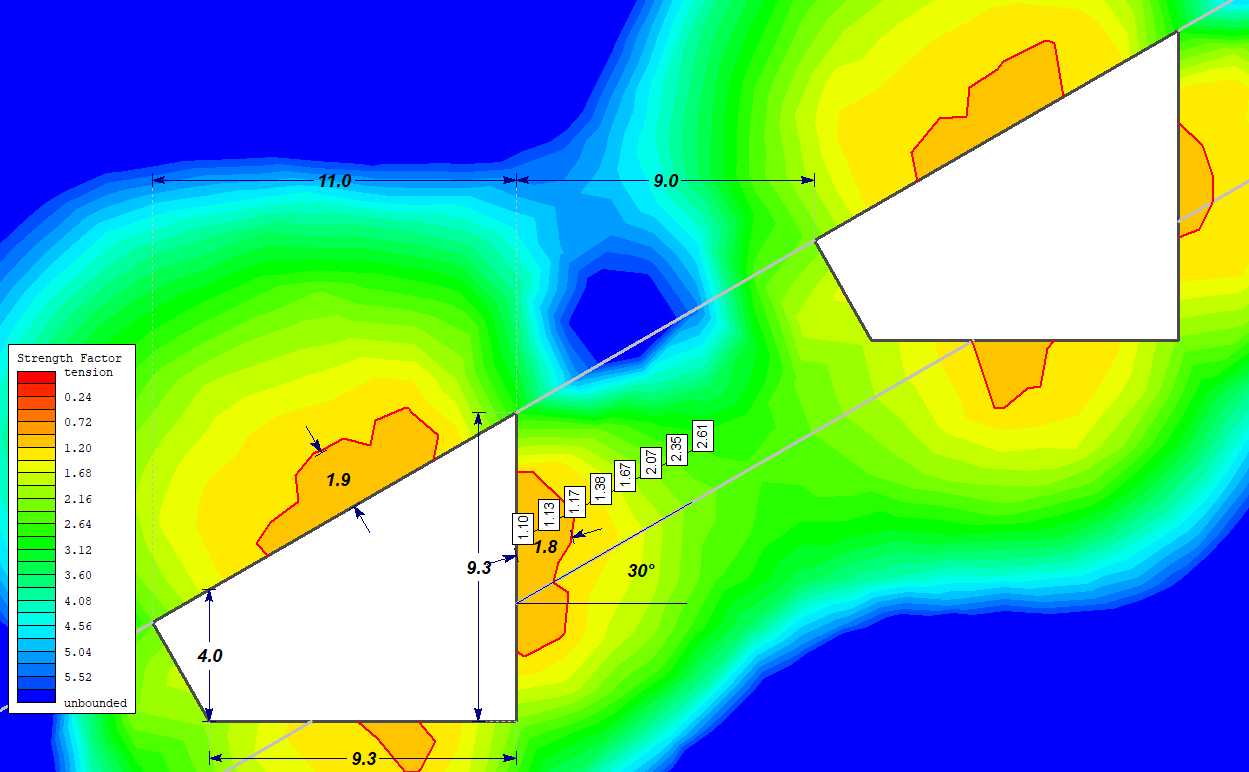
\includegraphics[width=0.8\textwidth]{assets/291}
	\caption*{}
\end{figure}

{\bfseries Рис. 11 -- Коэффициент запаса прочности законтурного массива при
параметрах очистной камеры 11х9 м и при угле падения 30 градусов}

\begin{figure}[H]
	\centering
	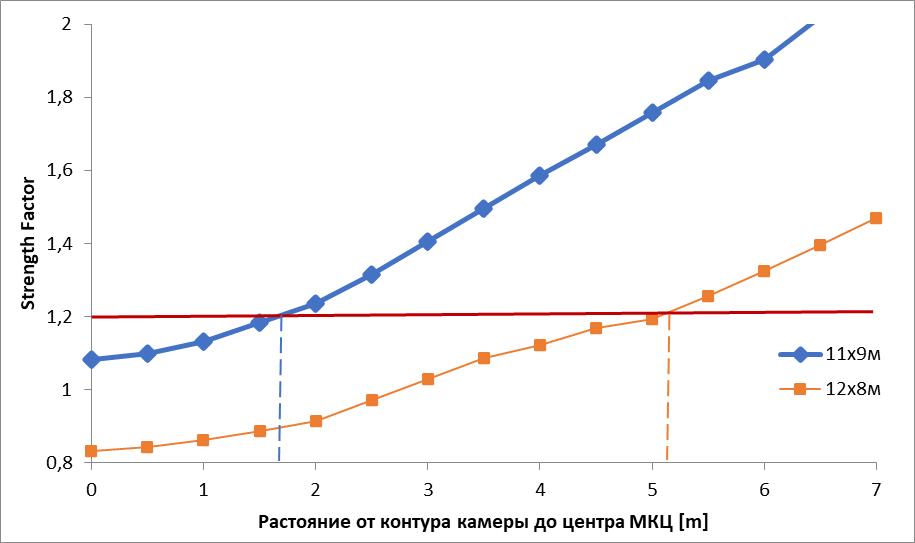
\includegraphics[width=0.8\textwidth]{assets/292}
	\caption*{}
\end{figure}

{\bfseries Рис. 12 -- Изменение коэффициента запаса прочности МКЦ}

На рисунках 13-14 представлены результаты численного моделирования
массива горных пород при угле падения залежей 35 градусов.

\begin{figure}[H]
	\centering
	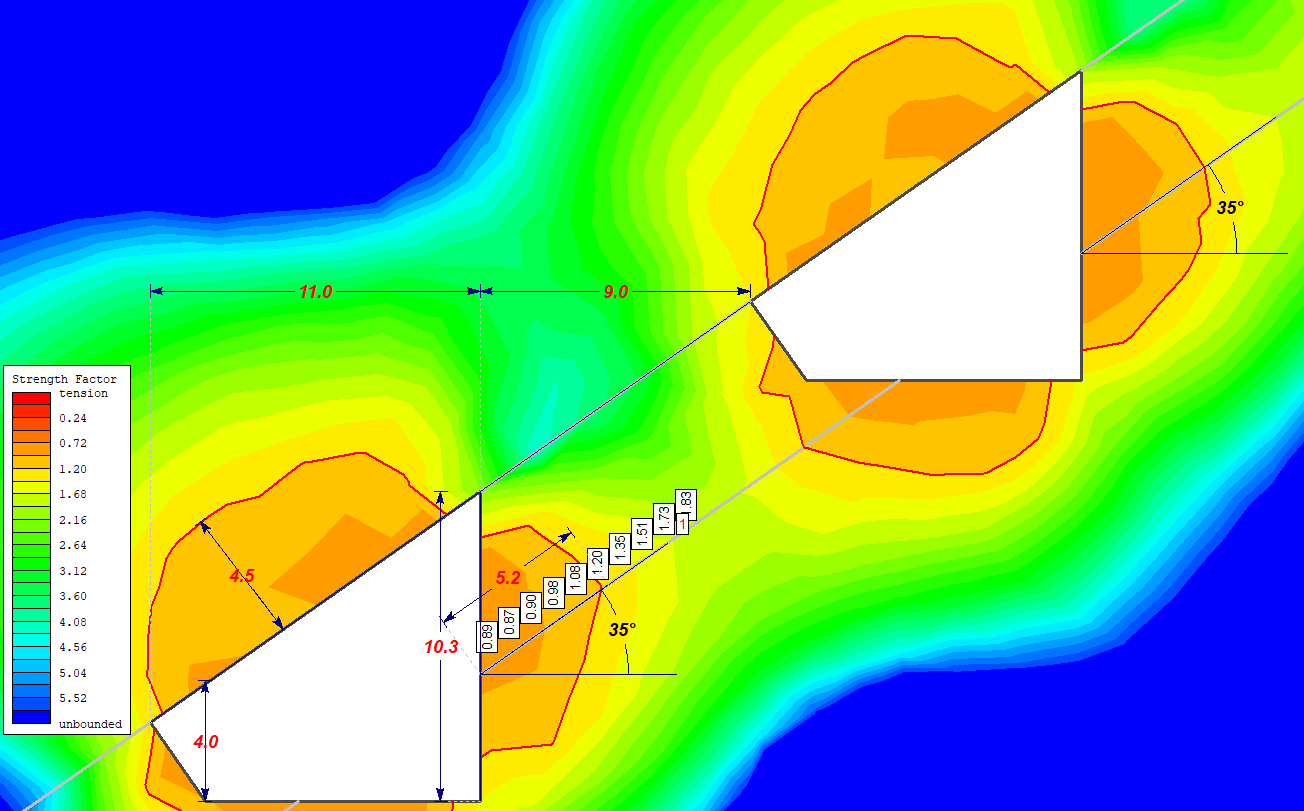
\includegraphics[width=0.8\textwidth]{assets/293}
	\caption*{}
\end{figure}

{\bfseries Рис. 13 -- Коэффициент запаса прочности законтурного массива при
параметрах очистной камеры 11х9 м и при угле падения 35 градусов}

По результатам численного моделирования при угле падения горных пород 35
градусов коэффициент запаса прочности МКЦ трапециевидной формы мощностью
9 метров и при ширине очистной камеры 11 метров (рис. 13) разрушение МКЦ
могут достигать до 5,2 метров, а обрушение кровли могут достигать до 4,5
метров, что ниже допустимых значений. Из чего следует предполагать, МКЦ
не устойчив и вероятность разрушения весьма велика {[}7{]}.

На рисунке 14 представлены результаты моделирования при параметрах
очистной камеры и МКЦ 10х10 м. В данном случае разрушение МКЦ не
превышает 2,2 метра, а обрушение горных пород по кровле не превышает 1,7
метров.

Для более детального сравнение результатов численного моделирования
выполненных методами конечных элементов построена график сравнение
коэффициента запаса прочности, представленного на рисунке 15.

\begin{figure}[H]
	\centering
	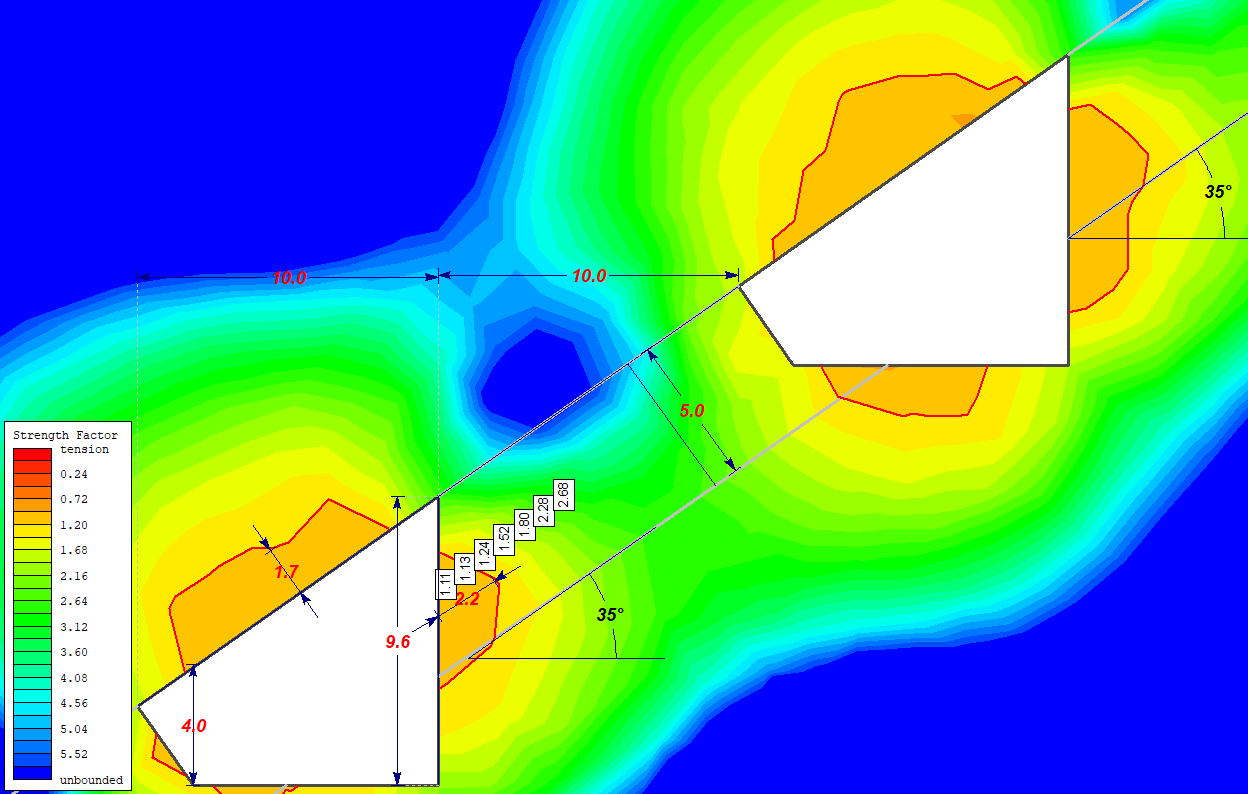
\includegraphics[width=0.8\textwidth]{assets/294}
	\caption*{}
\end{figure}

{\bfseries Рис. 14 -- Коэффициент запаса прочности законтурного массива при
параметрах очистной камеры 10х10 м и при угле падения 35 градусов}

\begin{figure}[H]
	\centering
	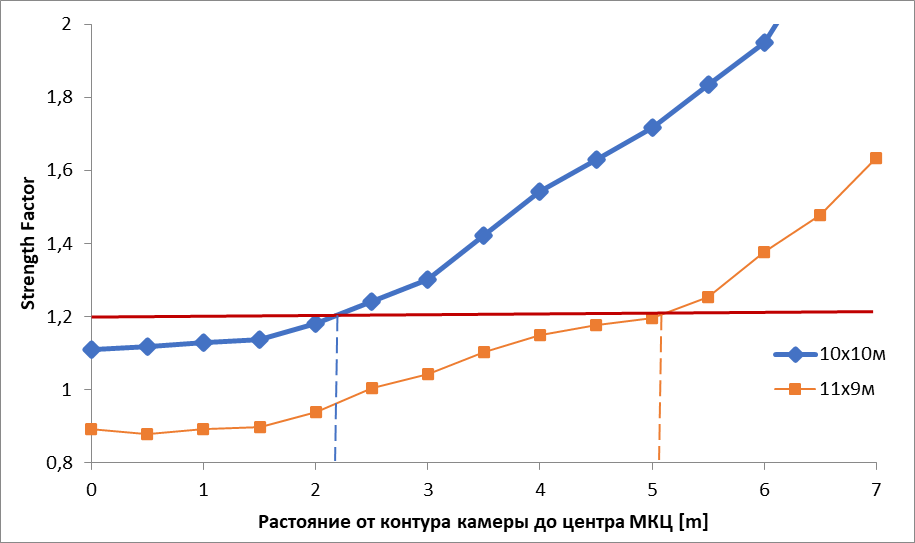
\includegraphics[width=0.8\textwidth]{assets/295}
	\caption*{}
\end{figure}

{\bfseries Рис. 15 -- Изменение коэффициента запаса прочности МКЦ}

В соответствии анализа результатов численного моделирования массива
горных пород методом конечных элементов построены несколько графиков
зависимости, первый из которых приведен на рисунке 16.

{\bfseries Рис. 16 -- График зависимости запаса прочности от GSI и угла
падения (при прямоугольной форме МКЦ)}

Данный график наглядно показывает, что МКЦ прямоугольной формы допустима
только в случае, если угол падения 20 градусов и GSI не менее 50 \%, в
остальных случаях горный массив не устойчив и вероятность обрушения МКЦ
весьма велика.

На следующем рисунке 17 представлены аналогичный график зависимости,
только для трапециевидной формы МКЦ мощностью 10 метров. Данный график
построен на основе интерпретации данных численного анализа МКЭ. Был
выполнен анализ с различными вариантами GSI.

{\bfseries Рис. 17 -- График зависимости запаса прочности от GSI и угла
падения}

{\bfseries (при трапециевидной форме МКЦ)}

По полученным результатам видно, что коэффициент запаса прочности (SF)
напрямую зависит от рейтинга массива GSI и угла падения залежей {[}8{]}.

По графику видно, что трапециевидное форма МКЦ в целом обеспечивает
сохранность выработанного пространства и целиков при углах падения:

20 градусов -- обеспечивает сохранность МКЦ и камеры при GSI не менее
35\%;

25 градусов -- обеспечивает сохранность МКЦ и камеры при GSI не менее
40\%;

30 градусов -- обеспечивает сохранность МКЦ и камеры при GSI не менее
50\%;

35 градусов -- обеспечивает сохранность МКЦ и камеры при GSI не менее
63\%.

{\bfseries Выводы.} Для обоснования допустимых параметров очистных камер и
целиков был выполнен анализ данных полученных в результате численного
моделирования массива горных пород. На основе комплекса выполненных
исследовании определены допустимые параметры очистной камеры и
междукамерного целика в зависимости от угла залегания.

На основе численного моделирования массива горных пород углом падения
20-35 градусов методами конечных элементов в программе RS-2 и в
результате дальнейшего анализа полученных данных о
напряженно-деформационного состояния были построены графики зависимости
позволяющие определять коэффициент запаса прочности (Strength Factor) в
зависимости от геологического индекса прочности (GSI) {[}9{]}.

Результаты моделирования показывает, что МКЦ классической (вертикальной)
формы мощностью 7 метров допустим только в случае, если угол падения
рудного тела 20-25 градусов и GSI не менее 50 \%, в остальных случаях
горный массив не устойчив и вероятность обрушения МКЦ {[}10{]} весьма
велика.

По результатам моделирования напряженного состояния следует, что в
окружающих выработку породах возникает зоны концентрация и разгрузки
напряжений. Она довольно быстро убывает вглубь массива, и на расстоянии
5-7 полупролетов выработки напряжения практически не отличаются от тех,
что действовали в массиве до проведения выработки.

\emph{{\bfseries Финансирование:} Научно-исследовательская работа выполнена
в рамках ГФ Министерством науки и высшего образования Республики
Казахстан №AP 19677938 по теме «Создание метода прогнозирования
сдвижения вмещающих пород до земной поверхности для модернизации
технологии повторной разработки пологих рудных залежей» на 2023-2025 гг.
Авторский коллектив также выражает благодарность руководству ТОО
«Корпорация Казахмыс» за предоставленную возможность проведения
исследовательских работ на базе предприятия. Особую благодарность
следует выразить редакторам и рецензентам журнала за их ценные советы,
которые были учтены для улучшения качества публикации.}

{\bfseries Литература}

1. Отчет о научно-исследовательской работе: Геомеханическое обоснование
отработки месторождений Жиландинской группы {[}док.внутреннего
пользования{]} / ТОО «Expert PRO». - Сатпаев-Усть-Каменогорск, 2022 .

2. Shichuan Zhang, Yangyang Li, Baotang Shen, Xizhen Sun, Liqun Gao.
Effective evaluation of pressure relief drilling for reducing rock
bursts and its application in underground coal mines // International
Journal of Rock Mechanics and Mining Sciences.). -2019. Vol. 114(11).
-P. 7-16. DOI 10.1016/j.ijrmms.2018.12.010

3. Read John \& Stacey Peter. Guidelines for Open Pit Slope Design. --
2009. DOI 10.1071/9780643101104

4. Технологическая инструкция по применению камерно-столбовой системы
разработки {[}док.внутреннего пользования{]} /ТОО «Корпорация Казахмыс».
- Жезказган, 2017.

5. Zhienbayev, A., Zharaspaev, M., Balpanova, M., Nurkasyn, N., Asanova,
Z., Zhakupov, B. Analysis of the roof span stabil-ity in terms of
room-and-pillar system of ore deposit mining// Mining of Mineral
Deposits. -- 2023. Vol. 17(1). - P. 129--137. DOI
10.33271/mining17.01.129

6. Mahdevari, Satar \& Shahriar, Kourosh \& Sharifzadeh, Mostafa \&
Tannant, Dwayne. (2017). Stability prediction of gate roadways in
longwall mining using artificial neural networks // Neural Computing and
Applications. -2016. -Vol. 28. -P. 3537-3555. DOI
10.1007/s00521-016-2263-2

7. Fitsak V.V., Lomakina E.S., Strakhova A.A. and Chernobai V.I.
Determination of Room-and-Pillar system parameters for Transition to
Greater Depths// International Journal of Applied Engineering Research.
-- 2017. -- Vol. 12(22). -P. 12322-12331.

8. Ivadilinova, D. \& Issabek, T. \& Takhanov, D. \& Yeskenova, Gulnura.
Predicting underground mining impact on the earth's sur-face // Naukovyi
Visnyk Natsionalnoho Hirnychoho Universytetu. -2023. --P. 32-37. DOI
10.33271/nvngu/2023-1/032

9. Félix Del Pozo, Eduardo Córdova, Carlos Marquardt, Rodolfo Cabezas G,
Philip Benson, Nick Koor, John Browning, Rocío Rudloff, Development of a
geomechanical model based on suitable estimations of GSI and UCS in
mining production slopes at the TilTil district, central Chile //
International Journal of Rock Mechanics and Mining Sciences. - 2023. -
Vol. 167(3). DOI 10.1016/j.ijrmms.2023.105390

10. Serebryakov E.V., Gladkov A.S. Geological and structural
characteristics of deep-level rock mass of the Udachnaya pipe deposit //
Journal of Mining Institute. - 2021. - Vol. 250. - P. 512-525. DOI
10.31897/PMI.2021.4.4

{\bfseries References}

1. Otchet o nauchno-issledovatel\textquotesingle skoi rabote:
Geomekhanicheskoe obosnovanie otrabotki mestorozhdenii Zhilandinskoi
gruppy {[}dok.vnutrennego pol\textquotesingle zovaniya{]} / TOO «Expert
PRO». - Satpaev-Ust\textquotesingle-Kamenogorsk, 2022.

2. Shichuan Zhang, Yangyang Li, Baotang Shen, Xizhen Sun, Liqun Gao.
Effective evaluation of pressure relief drilling for reducing rock
bursts and its application in underground coal mines // International
Journal of Rock Mechanics and Mining Sciences.). -2019. Vol. 114(11).
-P. 7-16. DOI 10.1016/j.ijrmms.2018.12.010

3. Read John \& Stacey Peter. Guidelines for Open Pit Slope Design. --
2009. DOI 10.1071/9780643101104

4. Tekhnologicheskaya instruktsiya po primeneniyu kamerno-stolbovoi
sistemy razrabotki {[}dok.vnutrennego pol\textquotesingle zovaniya{]}
/TOO «Korporatsiya Kazakhmys». - Zhezkazgan, 2017.

5. Zhienbayev, A., Zharaspaev, M., Balpanova, M., Nurkasyn, N., Asanova,
Z., Zhakupov, B. Analysis of the roof span stabil-ity in terms of
room-and-pillar system of ore deposit mining// Mining of Mineral
Deposits. -- 2023. Vol. 17(1). - P. 129--137. DOI
10.33271/mining17.01.129

6. Mahdevari, Satar \& Shahriar, Kourosh \& Sharifzadeh, Mostafa \&
Tannant, Dwayne. (2017). Stability prediction of gate roadways in
longwall mining using artificial neural networks // Neural Computing and
Applications. -2016. -Vol. 28. -P. 3537-3555. DOI
10.1007/s00521-016-2263-2

7. Fitsak V.V., Lomakina E.S., Strakhova A.A. and Chernobai V.I.
Determination of Room-and-Pillar system parameters for Transition to
Greater Depths// International Journal of Applied Engineering Research.
-- 2017. -- Vol. 12(22). -P. 12322-12331.

8. Ivadilinova, D. \& Issabek, T. \& Takhanov, D. \& Yeskenova, Gulnura.
Predicting underground mining impact on the earth's sur-face // Naukovyi
Visnyk Natsionalnoho Hirnychoho Universytetu. -2023. --P. 32-37. DOI
10.33271/nvngu/2023-1/032

9. Félix Del Pozo, Eduardo Córdova, Carlos Marquardt, Rodolfo Cabezas G,
Philip Benson, Nick Koor, John Browning, Rocío Rudloff, Development of a
geomechanical model based on suitable estimations of GSI and UCS in
mining production slopes at the TilTil district, central Chile //
International Journal of Rock Mechanics and Mining Sciences. - 2023. -
Vol. 167(3). DOI 10.1016/j.ijrmms.2023.105390

10. Serebryakov E.V., Gladkov A.S. Geological and structural
characteristics of deep-level rock mass of the Udachnaya pipe deposit //
Journal of Mining Institute. - 2021. - Vol. 250. - P. 512-525. DOI
10.31897/PMI.2021.4.4

\emph{{\bfseries Information about the authors}}

D.K. Takhanov - Candidate of Technical Sciences, Karaganda Technical
University named after Abylkas Saginov, Karaganda, Kazakhstan, e-mail:
takhanov80@mail.ru;

Balpanova M.J. - PhD, Karaganda Technical University named after Abylkas
Saginov, Karaganda, Kazakhstan, e-mail: balpanova86@mail.ru;

Ivadilinova D.T. - PhD, Karaganda Technical University named after
Abylkas Saginov, Karaganda, Kazakhstan, e-mail: dinulb@mail.ru.

\emph{{\bfseries Сведения об авторах}}

Таханов Д.К. - кандидат технических наук, Карагандинский технический
университет имени Абылкаса Сагинова, Караганда, Казахстан, e-mail:
takhanov80@mail.ru;

Балпанова М.Ж. - доктор PhD, Карагандинский технический университет
имени Абылкаса Сагинова, Караганда, Казахстан, e-mail:
balpanova86@mail.ru;

Ивадилинова Д.Т. - доктор PhD, Карагандинский технический университет
имени Абылкаса Сагинова, Караганда, Казахстан, e-mail: dinulb@mail.ru.\newpage
{\bfseries МРНТИ 52.45.19}

{\bfseries ВЛИЯНИЕ УЛЬТРАТОНКОГО ИЗМЕЛЬЧЕНИЯ НА ТЕХНОЛОГИЧЕСКИЕ ПОКАЗАТЕЛИ
ОБОГАЩЕНИЯ ОТВАЛЬНЫХ ХВОСТОВ}

{\bfseries \textsuperscript{1}А.Р. Мамбеталиева, \textsuperscript{1}Г.К.
Макашева\textsuperscript{🖂},\textsuperscript{1} Т.Ш. Тусупбекова,
\textsuperscript{2}С. К. Калиаскаров,}

{\bfseries \textsuperscript{2}С. Сагатбек}

\textsuperscript{1}Satbayev University, Алматы, Казахстан,

\textsuperscript{2}ТОО «КазГидроМедь»,Караганда, Казахстан

{\bfseries \textsuperscript{🖂}}Корреспондент-автор: mguldanka@mail.ru

Проблемы, с которым приходится сталкиваться горнодобывающей
промышленности для достижения утилизации отвальных хвостов в
соответствии с принципами экономики замкнутого цикла, включает в себя
улучшение довольно ограниченных знаний о минералогии, концентрации
примесей и объём хвостов в хвостохранилищах. Также необходимо разработка
технологий, чтобы сделать процесс экономически целесообразным. Для
улучшения показателей операции измельчения и оказать существенное
влияние на обогащение ценных компонентов было изучена влияния
ультратонкого измельчения на степень раскрываемости медных минералов
отвальных хвостов.

На основании оптико-минералогических исследований установлено, что
абсолютно раскрытые зерна халькопирита составляют не более 35 \% от
общего количества зерен, их размер в основном (на 60 \% отн.) в пределах
класса 10-45 мкм. Анализ ситовых характеристик хвостов после
ультратонкого измельчения показывает, что наибольшая концентрация меди
приходится на самый тонкий класс -0,006+0 мм, что свидетельствует о
высоком раскрытии медных минералов за счет ультратонкого измельчения.
Флотационные тесты по определению влияния степени ультратонкого
измельчения показала, что с увеличением тонины помола по классу
крупности -- 0,045 + 0 мм до 86 \% повышается извлечения меди с 66,49 до
73,52 \%; золота 71,07 до 77,78 \%; серебро 70,29 до 76,71 \%.

{\bfseries Ключевые слова:} обогащение полезных ископаемых, флотация,
ультратонкое измельчения, отвальные хвосты, халькопирит,
минералогический анализ.

{\bfseries УЛЬТРА ҰСАҚ ҰНТАҚТАУДЫҢ ҮЙІНДІ ҚАЛДЫҚТАРДЫҢ БАЙЫТУДЫҢ
ТЕХНОЛОГИЯЛЫҚ КӨРСЕТКІШТЕРІНЕ ӘСЕРІ}

{\bfseries \textsuperscript{1}А.Р. Мамбеталиева, \textsuperscript{1}Г.К.
Макашева\textsuperscript{🖂},\textsuperscript{1} Т.Ш. Тусупбекова,
\textsuperscript{2}С. К. Калиаскаров,}

{\bfseries \textsuperscript{2}С. Сагатбек}

\textsuperscript{1}Satbayev University, Алматы, Қазахстан,

\textsuperscript{2}«ҚазГидроМедь» ЖШС,Қарағанды, Қазахстан,

e-mail: mguldanka@mail.ru;

Айналмалы экономика қағидаларына сәйкес үйінді қалдықтарды кәдеге
жаратуға қол жеткізу үшін тау-кен өнеркәсібінің алдында тұрған мәселелер
минералогия, қоспалардың концентрациясы және қалдық қоймаларындағы
қалдықтардың көлемі туралы шектеулі білімді жақсартуды қамту қажет.
Процесті экономикалық тұрғыдан тиімді ету үшін технологияны дамыту
қажет. Ұнтақтау операциясының көрсеткіштерін жақсарту және құнды
компоненттерді байытуға айтарлықтай әсер ету үшін ультра жұқа
ұнтақтаудың үйінді қалдықтарының мыс минералдарының ашылу дәрежесіне
әсері зерттелді.

Оптикалық-минералогиялық зерттеулер негізінде мүлдем ашылған халькопирит
дәндері дәндердің жалпы санының 35\% - дан аспайтыны, олардың мөлшері
негізінен (60\% - ға) құрайтыны анықталды.) 10-45 мкм класс шегінде.
Ультра жұқа ұнтақтаудан кейін құйрықтардың елеуіш сипаттамаларын талдау
мыстың ең жоғары концентрациясы -0,006+0 мм ең жұқа класқа жататынын
көрсетеді, бұл ультра жұқа ұнтақтау арқылы мыс минералдарының жоғары
ашылуын көрсетеді. Ультра ұсақ ұнтақтау дәрежесінің әсерін анықтау
бойынша флотациялық сынақтар ұнтақтау тоннасының ұлғаюымен ұсақтау класы
бойынша -- 0,045 + 0 мм-ден 86\% - ға дейін мыс алу 66,49-дан 73,52\% -
ға дейін; алтын 71,07-ден 77,78\% - ға дейін; күміс 70,29-дан 76,71\% -
ға дейін артқанын көрсетті.

{\bfseries Түйін сөздер:} пайдалы қазбаларды байыту, флотация, ультра жұқа
ұнтақтау, үиінді қалдықтар, халькопирит, минералогиялық талдау.

{\bfseries THE EFFECT OF ULTRAFINE GRINDING ON THE TECHNOLOGICAL PARAMETERS
OF THE ENRICHMENT OF DUMP TAILINGS}

{\bfseries \textsuperscript{1}A.R. Mambetaliyeva, \textsuperscript{1}G.K.
Makasheva\textsuperscript{🖂}, \textsuperscript{1}T.Sh Tusupbekova,
\textsuperscript{2}S.K. Kaliaskarov,}

{\bfseries \textsuperscript{2}S. Sagatbek}

\textsuperscript{1}Satbayev University, Almaty, Kazakhstan,

\textsuperscript{2}Research Engineer at Kazhydromed LLP, Karaganda,
Kazakhstan,

e-mail: mguldanka@mail.ru;

The challenges that the mining industry has to face in order to achieve
tailings disposal in accordance with the principles of a closed-loop
economy include improving rather limited knowledge about mineralogy,
impurity concentrations and tailings volume in tailings dumps. It is
also necessary to develop technologies to make the process economically
feasible. In order to improve the performance of the grinding operation
and have a significant impact on the enrichment of valuable components,
the effects of ultrathin grinding on the degree of disclosure of copper
minerals of dump tailings were studied.

Based on optical and mineralogical studies, it was found that the
completely uncovered chalcopyrite grains make up no more than 35\% of
the total number of grains, their size is mainly (by 60\% relative)
within the class of 10-45 microns. Analysis of the sieve characteristics
of the tailings after ultrathin grinding shows that the highest
concentration of copper falls on the thinnest class -0.006+0 mm, that
indicates a high disclosure of copper minerals due to ultrathin
grinding. Flotation tests to determine the effect of the degree of
ultrathin grinding showed that with an increase in the fineness of
grinding in the size class -- 0.045 + 0 mm to 86\%, the extraction of
copper increases from 66.49 to 73.52\%; gold 71.07 to 77.78\%; silver
70.29 to 76.71\%.

{\bfseries Key words:} mineral processing, flotation, ultra-fine grinding,
waste tailings, chalcopyrite, mineralogical analysis.

{\bfseries Введение.} В настоящее время измельчение играет жизненно важную
роль в различных областях, включая горнодобывающую, химическую,
цементную и строительную промышленность. Для обогащения полезных
ископаемых подготовительным является измельчение, целью которого
является завершение мономерного отделения ценных минералов от пустых, и
получение квалифицированного материала для дальнейшего обогащения
{[}1{]}. Технологическая производительность измельчения фактически
определяет производительность обогащения и качество продуктов, тем самым
напрямую влияя на показатель содержания концентрата {[}2{]}. По
сравнению со стальной шаровой средой, керамическая шаровая среда
обладает характеристиками хорошей износостойкости, высокой твердости и
низкой плотности, и, таким образом, может значительно снизить расход
мощности измельчения и мелющих тел при применении в мельницах с
перемешиванием мелющей среды {[}1,3,{]}. Кроме того, керамическая
шаровая среда может улучшить флотационные характеристики цветных и
благородных руд за счет восстановления ионов железа, образующихся при
измельчении {[}4{]}. Следовательно, улучшение показателей операции
измельчения может оказать существенно влияние на обогащение полезных
ископаемых.

По мере истощения крупнозернистых, легко перерабатываемых рудных тел
перерабатываются более вкрапленные, мелкозернистые руды. Адекватное
высвобождение ценных компонентов в мелкозернистой руде часто достигается
только после того, как размер частиц руды был уменьшен до уровня ниже
традиционной границы шаровой мельницы в 45 мкм {[}5{]}.

Процесс ультратонкого измельчения заключается в получении ультрамельких
частиц руды. Единого стандарта для размера ультрадисперсных частиц не
существует, но принято считать, что ультрадисперсные частицы
металлической руды составляют менее 10 мкм, а неметаллической руды --
менее 5 мкм {[}6{]}.

Актуальность утилизации отвальных хвостов и хвостохранилищ заключается в
следующем, что в настоящее время наблюдается общемировая тенденция --
переход к «sustainable mining» (устойчивым геотехнологиям), одним из
направлений которых является расширение использования техногенных
отходов {[}7,8,{]}.

Недавние исследования показали, что переработка отвальных хвостов
является выгодной при одновременном снижении воздействия горнодобывающей
промышленности {[}9{]}. Так же разработаны исследования по изучению
методов обогащения, а именно флотации для переработки лежалых медных
хвостов {[}10{]}. Кроме того, с экономической точки зрения переработка
отходов используется как способ повышения эффективности использования
ресурсов {[}11{]} или перехода к безотходному процессу.

Основной целью данной работы является изучение влияния ультратонкого
измельчения в целях разработки технологии вторичной переработки лежалых
хвостов Карагайлинской обогатительной фабрики с получением сырья,
пригодного для дальнейшей переработки.

{\bfseries Материалы и методы.} Объект исследования -- проба лежалых
отвальных хвостов Карагайлинской обогатительной фабрики, за
складированных в карьере «Главный».

Вещественный состав пробы определялся масс-спектральным анализом с
индуктивно связанной плазмой (ICP-MS), содержание золота и серебра -
пробирным анализом. Согласно результатам химического анализа, содержание
основных ценных компонентов составило: меди 0,23 \%, серебра 8,11 г/т,
золота 0,78 г/т, цинка 0,35 \%, свинца 0,10 \%.

Изучение рудных минералов проводилось в отраженном свете в полированных
аншлифах-брикетах, с применением микроскопа OLYMPUS BX 53, видеокамеры
SIMAGIS XS-3CU и программного обеспечения для анализа изображений
Минерал С7 компании SIAMS.

На основании оптико-минералогических исследований установлено, что в
минеральном составе пробы преобладают породообразующие минералы, общее
содержание которых составляет 78,85 \%.

Рудные минералы распределяются следующим образом:

\begin{itemize}
\item
  основной (преобладающий) − пирит (20 \%):
\item
  второстепенные − сфалерит (0,5 \%), халькопирит (0,35 \%);
\item
  редкие или единичные знаки − оксиды железа (ред. зн.), ковеллин (ред.
  зн.), гидроокислы железа (ед. зн.), галенит (ед. зн.), блеклые руды
  (ред. зн.):
\item
  минералы благородных металлов в пробе не визуализированы.
\end{itemize}

Халькопирит (0,35 \% абс.) является основной минеральной формой
нахождения меди в пробе. Образует как самостоятельные отдельности (см.
рисунок 1a), так и сростки с нерудными минералами (см. рисунок 1b),
сфалеритом и пиритом. В сфалерите образует эмульсионные включения
(рисунок 1с). В пирите выполняет трещинки катаклаза или встречается в
виде тонких пойкилитовых включений (см. рисунок 2d), иногда в тесной
ассоциации с блеклыми рудами.

Присутствие халькопирита в тесной ассоциации с пиритом, в том числе в
виде тонких включений может отрицательно сказываться на показателях
обогащения и на селективном выделении данных компонентов руды.

Абсолютно раскрытые зерна халькопирита составляют не более 35 \% от
общего количества зерен, их размер в основном (на 60 \% отн.) в пределах
класса 10-45 мкм.

% \begin{longtable}[]{@{}
%   >{\raggedright\arraybackslash}p{(\columnwidth - 2\tabcolsep) * \real{0.5203}}
%   >{\raggedright\arraybackslash}p{(\columnwidth - 2\tabcolsep) * \real{0.4797}}@{}}
% \toprule\noalign{}
% \begin{minipage}[b]{\linewidth}\raggedright
% \begin{figure}[H]
% 	\centering
% 	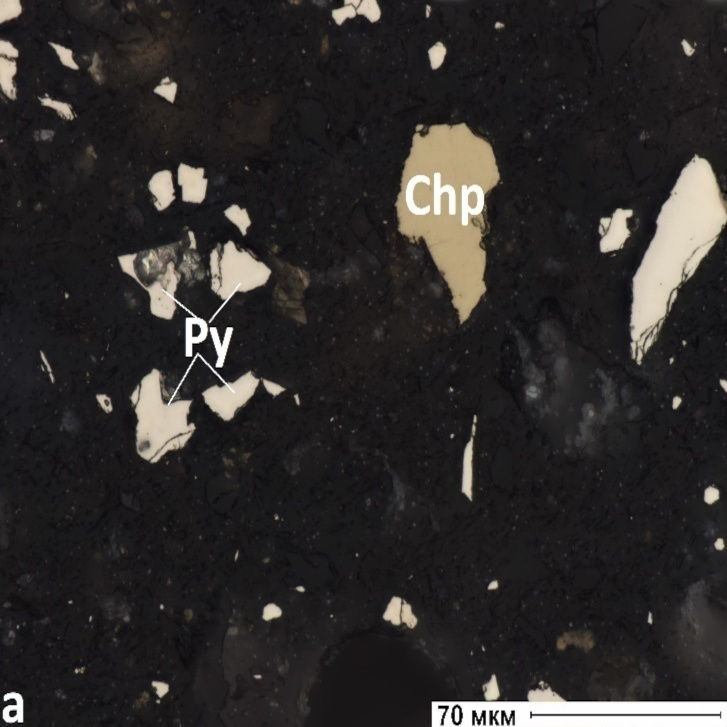
\includegraphics[width=0.8\textwidth]{assets/296}
% 	\caption*{}
% \end{figure}
% \end{minipage} & \begin{minipage}[b]{\linewidth}\raggedright
% \begin{figure}[H]
% 	\centering
% 	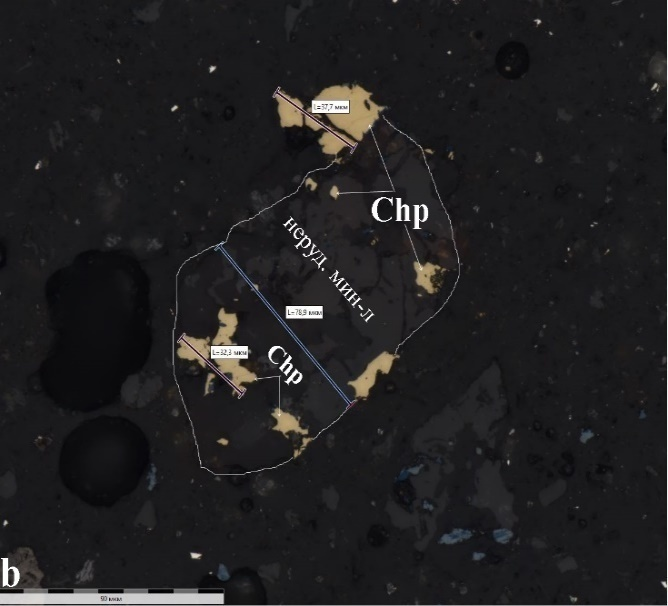
\includegraphics[width=0.8\textwidth]{assets/297}
% 	\caption*{}
% \end{figure}
% \end{minipage} \\
% \midrule\noalign{}
% \endhead
% \bottomrule\noalign{}
% \endlastfoot
% & \\
% \begin{figure}[H]
% 	\centering
% 	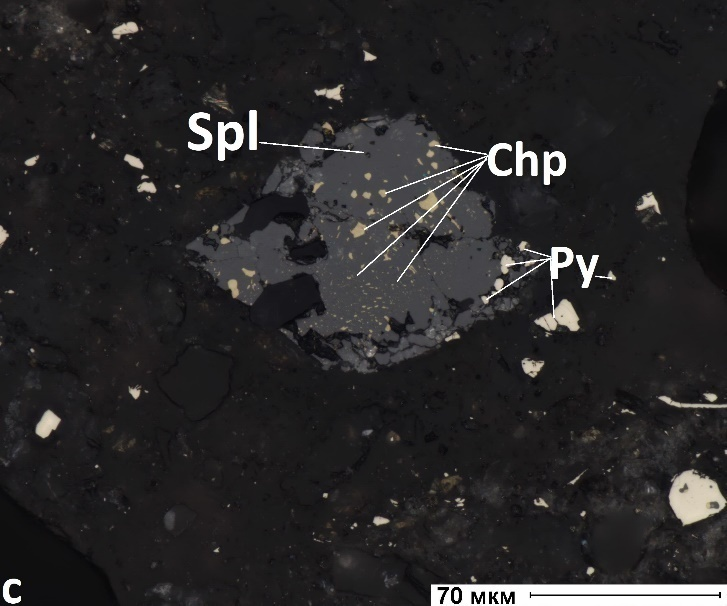
\includegraphics[width=0.8\textwidth]{assets/298}
% 	\caption*{}
% \end{figure} &
% \begin{figure}[H]
% 	\centering
% 	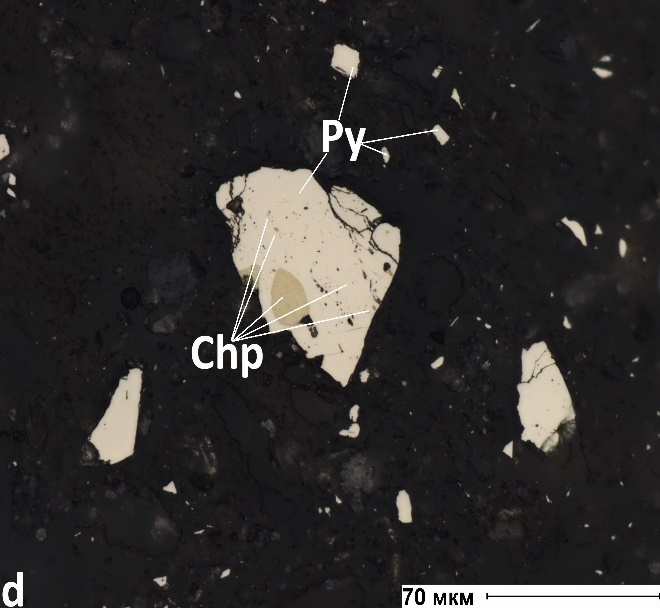
\includegraphics[width=0.8\textwidth]{assets/299}
% 	\caption*{}
% \end{figure} \\
% \multicolumn{2}{@{}>{\raggedright\arraybackslash}p{(\columnwidth - 2\tabcolsep) * \real{1.0000} + 2\tabcolsep}@{}}{%
% Chp-халькопирит, Spl-сфалерит, Py-пирит.
% 
% {\bfseries Рис. 1 -- Характеристика выделений халькопирита. Увел.
% 200/500}} \\
% \end{longtable}

Проведены исследования с использованием сверхтонкого измельчения в
лабораторной бисерной мельнице (далее МБЛ-1) по определению кинетики
измельчения исходной пробы отвальных хвостов контролем крупности
исходного продукта.

Известно, что использование тонкого и сверхтонкого помола продуктов,
содержащих благородные металлы, значительно увеличивает извлечение
золота и серебра в процессе обогащения. Но возможность моделирования
процесса измельчения в непрерывном режиме для бисерной мельницы является
основной проблемой на данный момент.

На рынке лабораторного оборудования представлен широкий ассортимент
лабораторных бисерных мельниц, зарубежных компании, среди разработок в
России -- это мельница МПБ -- 1 совместного российского-казахстанского
производства ТОО «SMAK Technology» и ООО БФК «Инжиниринг».

Лаборатории ООО "БФК Инжиниринг" и полупромышленные бисерные мельницы
имеют возможность моделировать технологический процесс ультратонкого
измельчения в поточном режиме {[}12{]}.

Внешний вид мельницы показаны на рисунке 2.

\begin{figure}[H]
	\centering
	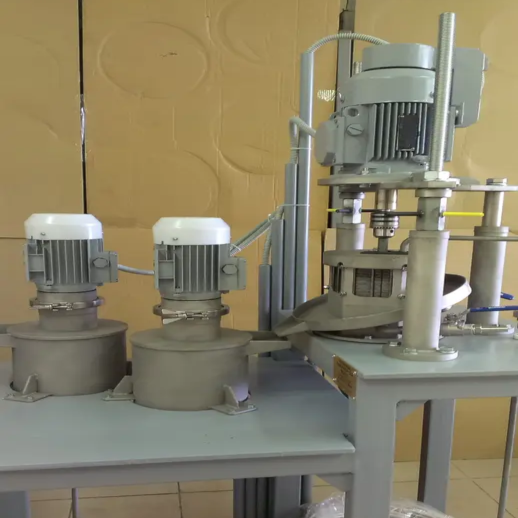
\includegraphics[width=0.8\textwidth]{assets/300}
	\caption*{}
\end{figure}

{\bfseries Рис. 2 -- Внешний вид бисерной мельницы МБЛ -- 1 для
сверхтонкого измельчения}

Флотационное обогащение выполнялось на стандартных лабораторных
пневмомеханических флотационных машинах типа Вэктис с объемом камер 3,
1.0 и 0.5 л.

Для исследования были применены следующие реагенты:

- сернистый натрий -- активатор;

- ксантогенат бутиловый - собиратель;

- МИБК -- пенообразователь;

Из вышеперечисленных реагентов приготавливались растворы необходимой
концентрации, с пересчетом на 100 \% активность, по формуле:

\[Р = \frac{V \bullet C}{A};\]

где V -- объем воды, мл; А -- активность, \%; C -- концентрация
реагента, д.е;

{\bfseries Результаты и обсуждение.} Результаты определения кинетики
измельчения исходной пробы хвостов c контролем крупности исходного
продукта представлены в таблице 1.

{\bfseries Таблица 1 -- Кинетика измельчения отвальных хвостов обогащения}

\begin{longtable}[]{@{}
  >{\raggedright\arraybackslash}p{(\columnwidth - 22\tabcolsep) * \real{0.1875}}
  >{\raggedright\arraybackslash}p{(\columnwidth - 22\tabcolsep) * \real{0.1031}}
  >{\raggedright\arraybackslash}p{(\columnwidth - 22\tabcolsep) * \real{0.0620}}
  >{\raggedright\arraybackslash}p{(\columnwidth - 22\tabcolsep) * \real{0.0732}}
  >{\raggedright\arraybackslash}p{(\columnwidth - 22\tabcolsep) * \real{0.0732}}
  >{\raggedright\arraybackslash}p{(\columnwidth - 22\tabcolsep) * \real{0.0620}}
  >{\raggedright\arraybackslash}p{(\columnwidth - 22\tabcolsep) * \real{0.0732}}
  >{\raggedright\arraybackslash}p{(\columnwidth - 22\tabcolsep) * \real{0.0732}}
  >{\raggedright\arraybackslash}p{(\columnwidth - 22\tabcolsep) * \real{0.0732}}
  >{\raggedright\arraybackslash}p{(\columnwidth - 22\tabcolsep) * \real{0.0732}}
  >{\raggedright\arraybackslash}p{(\columnwidth - 22\tabcolsep) * \real{0.0732}}
  >{\raggedright\arraybackslash}p{(\columnwidth - 22\tabcolsep) * \real{0.0732}}@{}}
\toprule\noalign{}
\multirow{2}{=}{\begin{minipage}[b]{\linewidth}\raggedright
Наименование продуктов, мм
\end{minipage}} &
\multirow{2}{=}{\begin{minipage}[b]{\linewidth}\raggedright
Выход, \%
\end{minipage}} &
\multicolumn{5}{>{\raggedright\arraybackslash}p{(\columnwidth - 22\tabcolsep) * \real{0.3436} + 8\tabcolsep}}{%
\begin{minipage}[b]{\linewidth}\raggedright
Содержание, \%
\end{minipage}} &
\multicolumn{5}{>{\raggedright\arraybackslash}p{(\columnwidth - 22\tabcolsep) * \real{0.3658} + 8\tabcolsep}@{}}{%
\begin{minipage}[b]{\linewidth}\raggedright
Распределение, \%
\end{minipage}} \\
& & \begin{minipage}[b]{\linewidth}\raggedright
Cu
\end{minipage} & \begin{minipage}[b]{\linewidth}\raggedright
Fe
\end{minipage} & \begin{minipage}[b]{\linewidth}\raggedright
S
\end{minipage} & \begin{minipage}[b]{\linewidth}\raggedright
Au
\end{minipage} & \begin{minipage}[b]{\linewidth}\raggedright
Ag
\end{minipage} & \begin{minipage}[b]{\linewidth}\raggedright
Cu
\end{minipage} & \begin{minipage}[b]{\linewidth}\raggedright
Fe
\end{minipage} & \begin{minipage}[b]{\linewidth}\raggedright
S
\end{minipage} & \begin{minipage}[b]{\linewidth}\raggedright
Au
\end{minipage} & \begin{minipage}[b]{\linewidth}\raggedright
Ag
\end{minipage} \\
\midrule\noalign{}
\endhead
\bottomrule\noalign{}
\endlastfoot
\multicolumn{12}{@{}>{\raggedright\arraybackslash}p{(\columnwidth - 22\tabcolsep) * \real{1.0000} + 22\tabcolsep}@{}}{%
Исходная проба} \\
+0,071 & 16,91 & 0,17 & 5,39 & 2,05 & 0,37 & 2,66 & 12,48 & 7,39 & 3,11
& 8,01 & 5,54 \\
-0,071 + 0,045 & 14,34 & 0,18 & 11,65 & 10,75 & 0,56 & 5,67 & 11,12 &
13,55 & 13,81 & 10,23 & 10,03 \\
-0,045 + 0,035 & 12,07 & 0,22 & 17,69 & 16,73 & 1,20 & 9,35 & 11,33 &
17,32 & 18,09 & 18,61 & 13,91 \\
-0,035+0,025 & 11,32 & 0,26 & 20,34 & 19,47 & 1,15 & 10,83 & 12,58 &
18,67 & 19,75 & 16,73 & 15,12 \\
-0,025+0,017 & 6,47 & 0,15 & 16,18 & 14,71 & 0,95 & 6,98 & 4,29 & 8,49 &
8,53 & 7,90 & 5,57 \\
-0,017+0,008 & 10,52 & 0,15 & 16,71 & 14,88 & 0,98 & 8,63 & 6,89 & 14,26
& 14,03 & 13,21 & 11,19 \\
-0,008+0,006 & 1,25 & 0,15 & 15,49 & 10,89 & 0,99 & 7,53 & 0,82 & 1,57 &
1,22 & 1,59 & 1,16 \\
-0,006+0 & 27,12 & 0,34 & 8,53 & 8,83 & 0,68 & 11,21 & 40,49 & 18,75 &
21,46 & 23,72 & 37,48 \\
Исходная проба & 100,0 & 0,23 & 12,33 & 11,16 & 0,78 & 8,11 & 100,0 &
100,0 & 100,0 & 100,0 & 100,0 \\
\multicolumn{12}{@{}>{\raggedright\arraybackslash}p{(\columnwidth - 22\tabcolsep) * \real{1.0000} + 22\tabcolsep}@{}}{%
Время измельчения 5 мин} \\
+0,071 & 10,61 & 0,21 & 4,87 & 3,08 & 0,28 & 3,2 & 9,76 & 4,19 & 2,93 &
3,81 & 4,18 \\
-0,071 + 0,045 & 3,14 & 0,47 & 28,11 & 30,14 & 1,76 & 18,34 & 6,47 &
7,16 & 8,48 & 7,09 & 7,10 \\
-0,045 + 0,035 & 12,01 & 0,13 & 15,27 & 14,62 & 1,02 & 9,14 & 6,96 &
14,87 & 15,73 & 15,75 & 13,53 \\
-0,035+0,025 & 20,70 & 0,2 & 13,43 & 12,7 & 0,8 & 7,71 & 17,56 & 22,54 &
23,56 & 21,11 & 19,68 \\
-0,025+0,017 & 5,47 & 0,17 & 12,44 & 11,34 & 0,75 & 7,32 & 4,07 & 5,52 &
5,56 & 5,28 & 4,94 \\
-0,017+0,008 & 10,60 & 0,16 & 11,29 & 10,01 & 0,7 & 6,2 & 7,22 & 9,71 &
9,51 & 9,46 & 8,11 \\
-0,008+0,006 & 0,49 & 0,16 & 10,06 & 7,98 & 0,73 & 5,47 & 0,34 & 0,40 &
0,35 & 0,46 & 0,33 \\
-0,006+0 & 36,98 & 0,3 & 11,87 & 10,22 & 0,78 & 9,24 & 47,62 & 35,61 &
33,88 & 37,04 & 42,13 \\
Исходная проба & 100,0 & 0,23 & 12,33 & 11,16 & 0,78 & 8,11 & 100,0 &
100,0 & 100,0 & 100,0 & 100,0 \\
\multicolumn{12}{@{}>{\raggedright\arraybackslash}p{(\columnwidth - 22\tabcolsep) * \real{1.0000} + 22\tabcolsep}@{}}{%
Время измельчения 10 мин} \\
+0,071 & 8,60 & 0,22 & 3,64 & 1,78 & 0,35 & 2,08 & 8,10 & 2,54 & 1,37 &
3,81 & 2,21 \\
-0,071 + 0,045 & 2,74 & 0,35 & 20,2 & 20,69 & 2,02 & 12,11 & 4,11 & 4,49
& 5,08 & 7,09 & 4,09 \\
-0,045 + 0,035 & 5,97 & 0,24 & 15,26 & 14,48 & 2,06 & 8,24 & 6,26 & 7,38
& 7,74 & 15,75 & 6,06 \\
-0,035+0,025 & 15,37 & 0,21 & 14,98 & 14,61 & 1,07 & 8,72 & 14,35 &
18,67 & 20,13 & 21,11 & 16,52 \\
-0,025+0,017 & 4,82 & 0,21 & 14,79 & 14,24 & 0,86 & 8,16 & 4,34 & 5,78 &
6,15 & 5,28 & 4,85 \\
-0,017+0,008 & 11,42 & 0,17 & 13,15 & 12,28 & 0,65 & 7,39 & 8,60 & 12,18
& 12,56 & 9,46 & 10,40 \\
-0,008+0,006 & 0,52 & 0,19 & 11,99 & 10,85 & 0,69 & 6,96 & 0,42 & 0,51 &
0,51 & 0,46 & 0,45 \\
-0,006+0 & 50,56 & 0,24 & 11,81 & 10,25 & 0,57 & 8,89 & 53,82 & 48,45 &
46,46 & 37,04 & 55,42 \\
Исходная проба & 100,0 & 0,23 & 12,33 & 11,16 & 0,78 & 8,11 & 100,0 &
100,0 & 100,0 & 100,0 & 100,0 \\
\multicolumn{12}{@{}>{\raggedright\arraybackslash}p{(\columnwidth - 22\tabcolsep) * \real{1.0000} + 22\tabcolsep}@{}}{%
Время измельчения 20 мин} \\
+0,071 & 5,33 & 0,20 & 3,71 & 1,89 & 0,25 & 2,03 & 4,52 & 1,60 & 0,90 &
1,70 & 1,33 \\
-0,071 + 0,045 & 3,07 & 0,37 & 22,43 & 23,69 & 1,52 & 13,17 & 4,90 &
5,58 & 6,51 & 5,97 & 4,98 \\
-0,045 + 0,035 & 3,58 & 0,25 & 15,83 & 15,64 & 0,99 & 9,14 & 3,95 & 4,59
& 5,01 & 4,55 & 4,03 \\
-0,035+0,025 & 10,02 & 0,21 & 14,78 & 14,45 & 0,97 & 7,93 & 9,12 & 12,01
& 12,97 & 12,47 & 9,80 \\
-0,025+0,017 & 3,67 & 0,19 & 14,19 & 13,61 & 0,95 & 7,67 & 3,03 & 4,22 &
4,47 & 4,45 & 3,47 \\
-0,017+0,008 & 9,10 & 0,16 & 12,65 & 11,65 & 0,84 & 6,63 & 6,53 & 9,34 &
9,50 & 9,82 & 7,44 \\
-0,008+0,006 & 0,63 & 0,22 & 12,06 & 10,75 & 0,81 & 6,66 & 0,61 & 0,62 &
0,61 & 0,65 & 0,52 \\
-0,006+0 & 64,62 & 0,24 & 11,84 & 10,37 & 0,73 & 8,59 & 67,34 & 62,03 &
60,03 & 60,39 & 68,42 \\
Исходная проба & 100,0 & 0,23 & 12,33 & 11,16 & 0,78 & 8,11 & 100,0 &
100,0 & 100,0 & 100,0 & 100,0 \\
\end{longtable}

Зависимость выхода класса крупности минус 0,006 мм от времени
ультратонкого измельчения показан на рисунке 3.

{\bfseries Рис. 3 -- Зависимость выхода класса -0,006 мм от времени
измельчения}

Анализ ситовых характеристик хвостов после ультратонкого измельчения
показывает, что наибольшая концентрация меди приходится на самый тонкий
класс -0,006+0 мм, и повышается в зависимости от времени измельчения с
47,62 \% (5 минут) до 67.34 \% (20 минут), что свидетельствует о высоком
раскрытии медных минералов за счет ультратонкого измельчения. Однако,
увеличение выхода тонкого класса -0,006+0 мм с 27,12 \% в исходных
хвостах (см. таблицу 1) до 64,42 \% может отрицательно сказываться на
показателях обогащения, за счет ошламования процесса.

Кроме того, в тонких классах вместе с медью концентрируется и железо,
что подтверждает тесную связь минералов меди с пиритом, которую не
удается разрушить даже при ультратонком измельчении.

С целью определения влияния степени ультратонкого измельчения на
извлечение меди и благородных металлов выполнены флотационные тесты.

Схема проведения опыта указана на рисунке 4. Условия опытов приведены в
таблице 2; результаты представлены на рисунке 5-7.

Концентрат 2

Хвосты

Основная Cu флотация

УТИ

Исходная проба

Контрольная флотация

Концентрат 2

{\bfseries Рис. 4 -- Лабораторная схема проведения опыта}

{\bfseries Таблица 2 -- Условия проведения опыта}

\begin{longtable}[]{@{}
  >{\raggedright\arraybackslash}p{(\columnwidth - 16\tabcolsep) * \real{0.2981}}
  >{\raggedright\arraybackslash}p{(\columnwidth - 16\tabcolsep) * \real{0.1195}}
  >{\raggedright\arraybackslash}p{(\columnwidth - 16\tabcolsep) * \real{0.0685}}
  >{\raggedright\arraybackslash}p{(\columnwidth - 16\tabcolsep) * \real{0.0963}}
  >{\raggedright\arraybackslash}p{(\columnwidth - 16\tabcolsep) * \real{0.0990}}
  >{\raggedright\arraybackslash}p{(\columnwidth - 16\tabcolsep) * \real{0.0946}}
  >{\raggedright\arraybackslash}p{(\columnwidth - 16\tabcolsep) * \real{0.0597}}
  >{\raggedright\arraybackslash}p{(\columnwidth - 16\tabcolsep) * \real{0.0747}}
  >{\raggedright\arraybackslash}p{(\columnwidth - 16\tabcolsep) * \real{0.0896}}@{}}
\toprule\noalign{}
\multirow{2}{=}{\begin{minipage}[b]{\linewidth}\raggedright
Операция
\end{minipage}} &
\multirow{2}{=}{\begin{minipage}[b]{\linewidth}\raggedright
Время,

мин
\end{minipage}} &
\multirow{2}{=}{\begin{minipage}[b]{\linewidth}\raggedright
рН
\end{minipage}} &
\multicolumn{5}{>{\raggedright\arraybackslash}p{(\columnwidth - 16\tabcolsep) * \real{0.4243} + 8\tabcolsep}}{%
\begin{minipage}[b]{\linewidth}\raggedright
Расход реагентов, г/т
\end{minipage}} & \begin{minipage}[b]{\linewidth}\raggedright
\end{minipage} \\
& & & \begin{minipage}[b]{\linewidth}\raggedright
МБС
\end{minipage} & \begin{minipage}[b]{\linewidth}\raggedright
Na\textsubscript{2}S
\end{minipage} & \begin{minipage}[b]{\linewidth}\raggedright
H\textsubscript{2}SO\textsubscript{4}
\end{minipage} & \begin{minipage}[b]{\linewidth}\raggedright
Кх
\end{minipage} & \begin{minipage}[b]{\linewidth}\raggedright
Aero 3418
\end{minipage} & \begin{minipage}[b]{\linewidth}\raggedright
МИБК
\end{minipage} \\
\begin{minipage}[b]{\linewidth}\raggedright
{\bfseries Всего:}
\end{minipage} & \begin{minipage}[b]{\linewidth}\raggedright
{\bfseries -}
\end{minipage} & \begin{minipage}[b]{\linewidth}\raggedright
{\bfseries -}
\end{minipage} & \begin{minipage}[b]{\linewidth}\raggedright
{\bfseries 800}
\end{minipage} & \begin{minipage}[b]{\linewidth}\raggedright
{\bfseries 150}
\end{minipage} & \begin{minipage}[b]{\linewidth}\raggedright
{\bfseries 7000}
\end{minipage} & \begin{minipage}[b]{\linewidth}\raggedright
{\bfseries 100}
\end{minipage} & \begin{minipage}[b]{\linewidth}\raggedright
{\bfseries 15}
\end{minipage} & \begin{minipage}[b]{\linewidth}\raggedright
{\bfseries 10}
\end{minipage} \\
\begin{minipage}[b]{\linewidth}\raggedright
Измельчение, -0,045 мм
\end{minipage} & \begin{minipage}[b]{\linewidth}\raggedright
5,10,20
\end{minipage} & \begin{minipage}[b]{\linewidth}\raggedright
-
\end{minipage} & \begin{minipage}[b]{\linewidth}\raggedright
800
\end{minipage} & \begin{minipage}[b]{\linewidth}\raggedright
-
\end{minipage} & \begin{minipage}[b]{\linewidth}\raggedright
-
\end{minipage} & \begin{minipage}[b]{\linewidth}\raggedright
-
\end{minipage} & \begin{minipage}[b]{\linewidth}\raggedright
-
\end{minipage} & \begin{minipage}[b]{\linewidth}\raggedright
-
\end{minipage} \\
\midrule\noalign{}
\endhead
\bottomrule\noalign{}
\endlastfoot
Основная Cu флотация & 10 & 7,7 & - & 150 & - & - & 15 & 5 \\
Контрольная флотация & 10 & 3,0 & - & - & 7000 & 100 & - & 5 \\
\end{longtable}

{\bfseries Рис. 5 - Результаты тестов по подбору степени измельчения для
медных минералов}

{\bfseries Рис. 6 - Зависимость извлечения золота от степени измельчения
отвальных хвостов обогащения}

{\bfseries Рис.7 - Зависимость извлечения серебра от степени измельчения
отвальных хвостов обогащения}

Из рисунков 5-7 следует, что с увеличением тонины помола по классу
крупности -0,045+0 мм с 69 до 86 \% наблюдается повышение извлечения
меди в суммарном концентрате на 7,03 \% (66,49 до 73,52 \%), также
повышается извлечения благородных металлов, золота на 6,71 \% (71,07 до
77,78 \%), серебро на 6,42 \% (70,29 \% до 76,71 \%).

{\bfseries Выводы.} Для расширения сырьевой базы и комплексного
использования сырья Казахстана принято решение о необходимости
рассмотрении возможности вторичной переработки отвальных хвостов
Карагайлинской обогатительной фабрики, за складированных в карьере
«Главный».

Выделение ценных компонентов из мелкозернистых руд часто достигается
только после того, как размер частицы руды снижается до уровня ниже
порового значения традиционной шаровой мельницы в - 0,045 мм.

Проведены исследования с использованием сверхтонкого измельчения в
лабораторной бисерной мельнице (далее МБЛ-1) по определению кинетики
измельчения исходной пробы отвальных хвостов контролем крупности
исходного продукта.

Чтобы определить влияние степени сверхтонкого измельчения на извлечение
меди и благородных металлов, были проведены флотационные тесты.

Из результатов представленный в графике 5-7 следует, что оптимальный
тонины помола по классу крупности -- 0,045 +0 мм 86 \%, при это
наблюдается увлечения извлечения меди в суммарной концентрат на 73,52
\%, золота на 77,78 \%, серебро на 76,71 \%.

{\bfseries Литература}

1. Xin Fang, Caibin Wu, Ningning Liao, Chengfang Yuan, Bin Xie, Jiaqi
Tong. The first attempt

of applying ceramic balls in industrial tumbling mill: A case study //
Minerals Engineering. 2022. Vol. 180. DOI 10.1016/j.mineng.2022.107504

2. Jean-Paul Duroudier Size Reduction of Divided Solids // 2 - Grinding
Energy. - 2016. - P. 53-72.

3.Paul Hassall, Emmanuel Nonnet,Ville Keikkala, Tarja Komminaho, Liisa
Kotila. Ceramic bead behavior in ultra-fine grinding mills // Minerals
Engineering. -2016. - Vol. 98. - P. 232-239.

4. Song Z.G., Corin K.C., Wiese J.G., O\textquotesingle Connor C.T.
Effect of different grinding media composition on the flotation of a PGM
ore // Minerals Engineering. -2018. - Vol. 124. -P. 74-76. DOI
10.1016/j.mineng.2018.05.014

5. Xiaolong Zhang, Yuexin Han, Yanjun Li, Wenbo Li, Jiancheng He,
Jianping Jin Strengthening the flotation recovery of silver using a
special ceramic-medium stirred mill // Powder Technology. -2022.- Vol.
406. DOI 10.1016/j.powtec.2022.117585

6. Caibin, W., Kuangdi, X. Ultrafine Grinding Process. In: Xu, K. (eds)
The ECPH Encyclopedia of Mining and Metallurgy. -Springer, Singapore,
2023. DOI: 10.1007/978-981-19-0740-1

7. Tuokuu F.X., Kpinpuo S.D., Hinson R.E. Sustainable development in
Ghana\textquotesingle s gold mines: clarifying the
stakeholder\textquotesingle s perspective // Journal of Sustainable
Mining.- 2019. -Vol. 18(2). - P. 77 - 84. DOI 10.1016/j.jsm.2019.02.007

8. Borujeni M.P., Gitinavard H., Evaluating the sustainable mining
contractor selection problems: An imprecise last aggregation preference
selection index method // Journal of Sustainable Mining. -2017.-Vol.
16(4).- P.207 - 218. DOI 10.1016/J.JSM.2017.12.006

9. Pier Paolo Manca, Giorgio Massacci, Davide Pintus, Giulio Sogos. The
flotation of sphalerite mine tailings as a remediation method// Minerals
Engineering. -2021. - Vol. 165.

DOI 10.1016/j.mineng.2021.106862

10. Kasongo K.B., Mwanat M. H., Ngamba Guellord , Merveille Kimpiab , K.
Fabrice Kapiamba. Statistical investigation of flotation parameters for
copper recovery from sulfide flotation tailings. // Results in
Engineering. -2021. - Vol. 9. DOI 10.1016/j.rineng.2021.100207

11. Malte Drobe, Frank Haubrich, Mariano Gajardo and Herwig Marbler.
Processing Tests, Adjusted Cost Models and the Economies ofReprocessing
Copper Mine Tailings in Chile. // Metals.- 2021. -Vol. 11. - P.
1031-1052. DOI:10.3390/met11010103

12.Сидоров И.А., Войлошников Г.И., Рубцов П.Н., Бондарь В.В., Грицай
С.Г. Испытания мельницы производства ООО «БФК Инжиниринг» для
ультратонкого измельчения упорных золотосодержащих сульфидных
концентратов // Горный информационно -- аналитический бюллетень
(научно-технический журнал). -2015. - С. 161 -- 166.

{\bfseries References}

1. Xin Fang, Caibin Wu, Ningning Liao, Chengfang Yuan, Bin Xie, Jiaqi
Tong. The first attempt of applying ceramic balls in industrial tumbling
mill: A case study // Minerals Engineering. 2022. Volume 180. DOI:
10.1016/j.mineng.2022.107504

2. Jean-Paul Duroudier Size Reduction of Divided Solids // 2 - Grinding
Energy. - 2016. -P. 53-72.

3. Paul Hassall, Emmanuel Nonnet,Ville Keikkala, Tarja Komminaho, Liisa
Kotila. Ceramic bead behavior in ultra-fine grinding mills // Minerals
Engineering. -2016. --Vol. 98. -P. 232-239.

4. Song Z.G., Corin K.C., Wiese J.G., O\textquotesingle Connor C.T.
Effect of different grinding media composition on the flotation of a PGM
ore // Minerals Engineering. -2018. --Vol. 124. -P. 74-76. DOI
10.1016/j.mineng.2018.05.014

5. Xiaolong Zhang, Yuexin Han, Yanjun Li, Wenbo Li, Jiancheng He,
Jianping Jin Strengthening the flotation recovery of silver using a
special ceramic-medium stirred mill // Powder Technology. -2022. - Vol.
406. DOI 10.1016/j.powtec.2022.117585

6. Caibin, W., Kuangdi, X. Ultrafine Grinding Process. In: Xu, K. (eds)
The ECPH Encyclopedia of Mining and Metallurgy. -Springer, Singapore,
2023. DOI 10.1007/978-981-19-0740-1

7. Tuokuu F.X., Kpinpuo S.D., Hinson R.E. Sustainable development in
Ghana\textquotesingle s gold mines: clarifying the
stakeholder\textquotesingle s perspective // Journal of Sustainable
Mining. - 2019. -Vol. 18(2). -P. 77--84. DOI: 10.1016/j.jsm.2019.02.007

8. Borujeni M.P., Gitinavard H., Evaluating the sustainable mining
contractor selection problems: An imprecise last aggregation preference
selection index method // Journal of Sustainable Mining.- 2017. -- Vol.
16(4).- P. 207--218. DOI 10.1016/J.JSM.2017.12.006

9. Pier Paolo Manca, Giorgio Massacci, Davide Pintus, Giulio Sogos. The
flotation of sphalerite mine tailings as a remediation method// Minerals
Engineering. -2021. - Vol. 165. DOI

10.1016/j.mineng.2021.106862

10. Kasongo K.B., Mwanat M. H., Ngamba Guellord , Merveille Kimpiab , K.
Fabrice Kapiamba. Statistical investigation of flotation parameters for
copper recovery from sulfide flotation tailings. // Results in
Engineering. -2021.-Vol. 9. DOI 10.1016/j.rineng.2021.100207

11. Malte Drobe, Frank Haubrich, Mariano Gajardo and Herwig Marbler.
Processing Tests, Adjusted Cost Models and the Economies ofReprocessing
Copper Mine Tailings in Chile. // Metals.- 2021. -Vol. 11. - P.
1031-1052. DOI 10.3390/met11010103

12. Sidorov I.A., Voiloshnikov G.I., Rubtsov P.N.,
Bondar\textquotesingle{} V.V., Gritsai S.G. Ispytaniya
mel\textquotesingle nitsy proizvodstva OOO «BFK Inzhiniring» dlya
ul\textquotesingle tratonkogo izmel\textquotesingle cheniya upornykh
zolotosoderzhashchikh sul\textquotesingle fidnykh kontsentratov //
Gornyi informatsionno -- analiticheskii byulleten\textquotesingle{}
(nauchno-tekhnicheskii zhurnal). -2015. - S. 161 -- 166. {[}in
Russian{]}

\emph{{\bfseries Сведения об авторах}}

Мамбеталиева А.Р. - доктор PhD, старший преподаватель кафедры
«Металлургии и обогащения полезных ископаемых» Satbayev University,
Алматы, Казахстан, e-mail: a.mambetaliyeva@satbayev.university;

Макашева Г.К. - докторант кафедры «Металлургии и обогащения полезных
ископаемых» Satbayev University, Алматы, Казахстан, e-mail:
mguldanka@mail.ru;

Тусупбекова Т.Ш. - докторант кафедры «Металлургии и обогащения полезных
ископаемых» Satbayev University, Алматы, Казахстан, e-mail:
tansholpan\_87.09@mail.ru;

Макашева Г.К. - докторант кафедры «Металлургии и обогащения полезных
ископаемых» Satbayev University, Алматы, Казахстан, e-mail:
mguldanka@mail.ru;

Калиаскаров С.К. - инженер-исследователь ТОО «КазГидроМедь», Караганда,
Казахстан, e-mail: sulya-95@mail.ru;

Сагатбек С. - магистр технических наук, инженер-исследователь ТОО
«КазГидроМедь», Караганда, Казахстан, e-mail: sunkar\_0396@mail.ru;

\emph{{\bfseries Information about the authors}}

Mambetaliyeva A.R. - PhD, Senior Lecturer at the Department of
Metallurgy and Mineral Processing at Satbayev University, Almaty,
Kazakhstan, e-mail: a.mambetaliyeva@satbayev.university;

Tusupbekova T.Sh. - doctoral student of the Department of Metallurgy and
Mineral Processing at Satbayev University, Almaty, Kazakhstan, e-mail:
tansholpan\_87.09@mail.ru;

Makasheva G. K., Doctoral student of the Department of Metallurgy and
Mineral Processing at Satbayev University, Almaty, Kazakhstan, e-mail:
mguldanka@mail.ru;

Kaliaskarov S.K.-Research Engineer at Kazhydromed LLP, Karaganda,
Kazakhstan, e-mail: sulya-95@mail.ru;

Sagatbek S. - Master of Technical Sciences, Research Engineer at
Kazhydromed LLP, Karaganda, Kazakhstan, e-mail: sunkar\_0396@mail.ru\newpage
{\bfseries МРНТИ }-- 52.45.19}

{\bfseries ВЛИЯНИЕ УЛЬТРАТОНКОГО ИЗМЕЛЬЧЕНИЯ НА ТЕХНОЛОГИЧЕСКИЕ ПОКАЗАТЕЛИ
ОБОГАЩЕНИЯ ОТВАЛЬНЫХ ХВОСТОВ}

{\bfseries \textsuperscript{1}А.Р. Мамбеталиева, \textsuperscript{1}Г.К.
Макашева\textsuperscript{🖂},\textsuperscript{1} Т.Ш. Тусупбекова,
\textsuperscript{2}С. К. Калиаскаров,}

{\bfseries \textsuperscript{2}С. Сагатбек}

\textsuperscript{1}Satbayev University, Алматы, Казахстан,

\textsuperscript{2}ТОО «КазГидроМедь»,Караганда, Казахстан

{\bfseries \textsuperscript{🖂}}Корреспондент-автор: mguldanka@mail.ru;

Проблемы, с которым приходится сталкиваться горнодобывающей
промышленности для достижения утилизации отвальных хвостов в
соответствии с принципами экономики замкнутого цикла, включает в себя
улучшение довольно ограниченных знаний о минералогии, концентрации
примесей и объём хвостов в хвостохранилищах. Также необходимо разработка
технологий, чтобы сделать процесс экономически целесообразным. Для
улучшения показателей операции измельчения и оказать существенное
влияние на обогащение ценных компонентов было изучена влияния
ультратонкого измельчения на степень раскрываемости медных минералов
отвальных хвостов.

На основании оптико-минералогических исследований установлено, что
абсолютно раскрытые зерна халькопирита составляют не более 35 \% от
общего количества зерен, их размер в основном (на 60 \% отн.) в пределах
класса 10-45 мкм. Анализ ситовых характеристик хвостов после
ультратонкого измельчения показывает, что наибольшая концентрация меди
приходится на самый тонкий класс -0,006+0 мм, что свидетельствует о
высоком раскрытии медных минералов за счет ультратонкого измельчения.
Флотационные тесты по определению влияния степени ультратонкого
измельчения показала, что с увеличением тонины помола по классу
крупности -- 0,045 + 0 мм до 86 \% повышается извлечения меди с 66,49 до
73,52 \%; золота 71,07 до 77,78 \%; серебро 70,29 до 76,71 \%.

{\bfseries Ключевые слова:} обогащение полезных ископаемых, флотация,
ультратонкое измельчения, отвальные хвосты, халькопирит,
минералогический анализ.

{\bfseries УЛЬТРА ҰСАҚ ҰНТАҚТАУДЫҢ ҮЙІНДІ ҚАЛДЫҚТАРДЫҢ БАЙЫТУДЫҢ
ТЕХНОЛОГИЯЛЫҚ КӨРСЕТКІШТЕРІНЕ ӘСЕРІ}

{\bfseries \textsuperscript{1}А.Р. Мамбеталиева, \textsuperscript{1}Г.К.
Макашева\textsuperscript{🖂},\textsuperscript{1} Т.Ш. Тусупбекова,
\textsuperscript{2}С. К. Калиаскаров,}

{\bfseries \textsuperscript{2}С. Сагатбек}

\textsuperscript{1}Satbayev University, Алматы, Қазахстан,

\textsuperscript{2}«ҚазГидроМедь» ЖШС,Қарағанды, Қазахстан,

e-mail: mguldanka@mail.ru

Айналмалы экономика қағидаларына сәйкес үйінді қалдықтарды кәдеге
жаратуға қол жеткізу үшін тау-кен өнеркәсібінің алдында тұрған мәселелер
минералогия, қоспалардың концентрациясы және қалдық қоймаларындағы
қалдықтардың көлемі туралы шектеулі білімді жақсартуды қамту қажет.
Процесті экономикалық тұрғыдан тиімді ету үшін технологияны дамыту
қажет. Ұнтақтау операциясының көрсеткіштерін жақсарту және құнды
компоненттерді байытуға айтарлықтай әсер ету үшін ультра жұқа
ұнтақтаудың үйінді қалдықтарының мыс минералдарының ашылу дәрежесіне
әсері зерттелді.

Оптикалық-минералогиялық зерттеулер негізінде мүлдем ашылған халькопирит
дәндері дәндердің жалпы санының 35\% - дан аспайтыны, олардың мөлшері
негізінен (60\% - ға) құрайтыны анықталды.) 10-45 мкм класс шегінде.
Ультра жұқа ұнтақтаудан кейін құйрықтардың елеуіш сипаттамаларын талдау
мыстың ең жоғары концентрациясы -0,006+0 мм ең жұқа класқа жататынын
көрсетеді, бұл ультра жұқа ұнтақтау арқылы мыс минералдарының жоғары
ашылуын көрсетеді. Ультра ұсақ ұнтақтау дәрежесінің әсерін анықтау
бойынша флотациялық сынақтар ұнтақтау тоннасының ұлғаюымен ұсақтау класы
бойынша -- 0,045 + 0 мм-ден 86\% - ға дейін мыс алу 66,49-дан 73,52\% -
ға дейін; алтын 71,07-ден 77,78\% - ға дейін; күміс 70,29-дан 76,71\% -
ға дейін артқанын көрсетті.

{\bfseries Түйін сөздер:} пайдалы қазбаларды байыту, флотация, ультра жұқа
ұнтақтау, үиінді қалдықтар, халькопирит, минералогиялық талдау.

{\bfseries THE EFFECT OF ULTRAFINE GRINDING ON THE TECHNOLOGICAL}

{\bfseries PARAMETERS OF THE ENRICHMENT OF DUMP TAILINGS}

{\bfseries \textsuperscript{1}A.R. Mambetaliyeva, \textsuperscript{1}G.K.
Makasheva\textsuperscript{🖂}, \textsuperscript{1}T.Sh Tusupbekova,
\textsuperscript{2}S.K. Kaliaskarov,}

{\bfseries \textsuperscript{2}S. Sagatbek}

\textsuperscript{1}Satbayev University, Almaty, Kazakhstan,

\textsuperscript{2}Research Engineer at Kazhydromed LLP, Karaganda,
Kazakhstan,

e-mail: mguldanka@mail.ru

The challenges that the mining industry has to face in order to achieve
tailings disposal in accordance with the principles of a closed-loop
economy include improving rather limited knowledge about mineralogy,
impurity concentrations and tailings volume in tailings dumps. It is
also necessary to develop technologies to make the process economically
feasible. In order to improve the performance of the grinding operation
and have a significant impact on the enrichment of valuable components,
the effects of ultrathin grinding on the degree of disclosure of copper
minerals of dump tailings were studied.

Based on optical and mineralogical studies, it was found that the
completely uncovered chalcopyrite grains make up no more than 35\% of
the total number of grains, their size is mainly (by 60\% relative)
within the class of 10-45 microns. Analysis of the sieve characteristics
of the tailings after ultrathin grinding shows that the highest
concentration of copper falls on the thinnest class -0.006+0 mm, that
indicates a high disclosure of copper minerals due to ultrathin
grinding. Flotation tests to determine the effect of the degree of
ultrathin grinding showed that with an increase in the fineness of
grinding in the size class -- 0.045 + 0 mm to 86\%, the extraction of
copper increases from 66.49 to 73.52\%; gold 71.07 to 77.78\%; silver
70.29 to 76.71\%.

{\bfseries Key words:} mineral processing, flotation, ultra-fine grinding,
waste tailings, chalcopyrite, mineralogical analysis.

{\bfseries Введение.} В настоящее время измельчение играет жизненно важную
роль в различных областях, включая горнодобывающую, химическую,
цементную и строительную промышленность. Для обогащения полезных
ископаемых подготовительным является измельчение, целью которого
является завершение мономерного отделения ценных минералов от пустых, и
получение квалифицированного материала для дальнейшего обогащения
{[}1{]}. Технологическая производительность измельчения фактически
определяет производительность обогащения и качество продуктов, тем самым
напрямую влияя на показатель содержания концентрата {[}2{]}. По
сравнению со стальной шаровой средой, керамическая шаровая среда
обладает характеристиками хорошей износостойкости, высокой твердости и
низкой плотности, и, таким образом, может значительно снизить расход
мощности измельчения и мелющих тел при применении в мельницах с
перемешиванием мелющей среды {[}3,4{]}. Кроме того, керамическая шаровая
среда может улучшить флотационные характеристики цветных и благородных
руд за счет восстановления ионов железа, образующихся при измельчении
{[}5{]}. Следовательно, улучшение показателей операции измельчения может
оказать существенно влияние на обогащение полезных ископаемых.

По мере истощения крупнозернистых, легко перерабатываемых рудных тел
перерабатываются более вкрапленные, мелкозернистые руды. Адекватное
высвобождение ценных компонентов в мелкозернистой руде часто достигается
только после того, как размер частиц руды был уменьшен до уровня ниже
традиционной границы шаровой мельницы в 45 мкм {[}6{]}.

Процесс ультратонкого измельчения заключается в получении ультрамельких
частиц руды. Единого стандарта для размера ультрадисперсных частиц не
существует, но принято считать, что ультрадисперсные частицы
металлической руды составляют менее 10 мкм, а неметаллической руды --
менее 5 мкм {[}7{]}.

Актуальность утилизации отвальных хвостов и хвостохранилищ заключается в
следующем, что в настоящее время наблюдается общемировая тенденция --
переход к «sustainable mining» (устойчивым геотехнологиям), одним из
направлений которых является расширение использования техногенных
отходов {[}8,9{]}.

Недавние исследования показали, что переработка отвальных хвостов
является выгодной при одновременном снижении воздействия горнодобывающей
промышленности {[}10{]}. Так же разработаны исследования по изучению
методов обогащения, а именно флотации для переработки лежалых медных
хвостов {[}11{]}. Кроме того, с экономической точки зрения переработка
отходов используется как способ повышения эффективности использования
ресурсов {[}12{]} или перехода к безотходному процессу.

Основной целью данной работы является изучение влияния ультратонкого
измельчения в целях разработки технологии вторичной переработки лежалых
хвостов Карагайлинской обогатительной фабрики с получением сырья,
пригодного для дальнейшей переработки.

{\bfseries Материалы и методы.} Объект исследования -- проба лежалых
отвальных хвостов Карагайлинской обогатительной фабрики, за
складированных в карьере «Главный».

Вещественный состав пробы определялся масс-спектральным анализом с
индуктивно связанной плазмой (ICP-MS), содержание золота и серебра -
пробирным анализом. Согласно результатам химического анализа, содержание
основных ценных компонентов составило: меди 0,23 \%, серебра 8,11 г/т,
золота 0,78 г/т, цинка 0,35 \%, свинца 0,10 \%.

Изучение рудных минералов проводилось в отраженном свете в полированных
аншлифах-брикетах, с применением микроскопа OLYMPUS BX 53, видеокамеры
SIMAGIS XS-3CU и программного обеспечения для анализа изображений
Минерал С7 компании SIAMS.

На основании оптико-минералогических исследований установлено, что в
минеральном составе пробы преобладают породообразующие минералы, общее
содержание которых составляет 78,85 \%.

Рудные минералы распределяются следующим образом:

\begin{itemize}
\item
  основной (преобладающий) − пирит (20 \%):
\item
  второстепенные − сфалерит (0,5 \%), халькопирит (0,35 \%);
\item
  редкие или единичные знаки − оксиды железа (ред. зн.), ковеллин (ред.
  зн.), гидроокислы железа (ед. зн.), галенит (ед. зн.), блеклые руды
  (ред. зн.):
\item
  минералы благородных металлов в пробе не визуализированы.
\end{itemize}

Халькопирит (0,35 \% абс.) является основной минеральной формой
нахождения меди в пробе. Образует как самостоятельные отдельности (см.
рисунок 1a), так и сростки с нерудными минералами (см. рисунок 1b),
сфалеритом и пиритом. В сфалерите образует эмульсионные включения
(рисунок 1с). В пирите выполняет трещинки катаклаза или встречается в
виде тонких пойкилитовых включений (см. рисунок 2d), иногда в тесной
ассоциации с блеклыми рудами.

Присутствие халькопирита в тесной ассоциации с пиритом, в том числе в
виде тонких включений может отрицательно сказываться на показателях
обогащения и на селективном выделении данных компонентов руды.

Абсолютно раскрытые зерна халькопирита составляют не более 35 \% от
общего количества зерен, их размер в основном (на 60 \% отн.) в пределах
класса 10-45 мкм.

% \begin{longtable}[]{@{}
%   >{\raggedright\arraybackslash}p{(\columnwidth - 2\tabcolsep) * \real{0.5203}}
%   >{\raggedright\arraybackslash}p{(\columnwidth - 2\tabcolsep) * \real{0.4797}}@{}}
% \toprule\noalign{}
% \begin{minipage}[b]{\linewidth}\raggedright
% \begin{figure}[H]
% 	\centering
% 	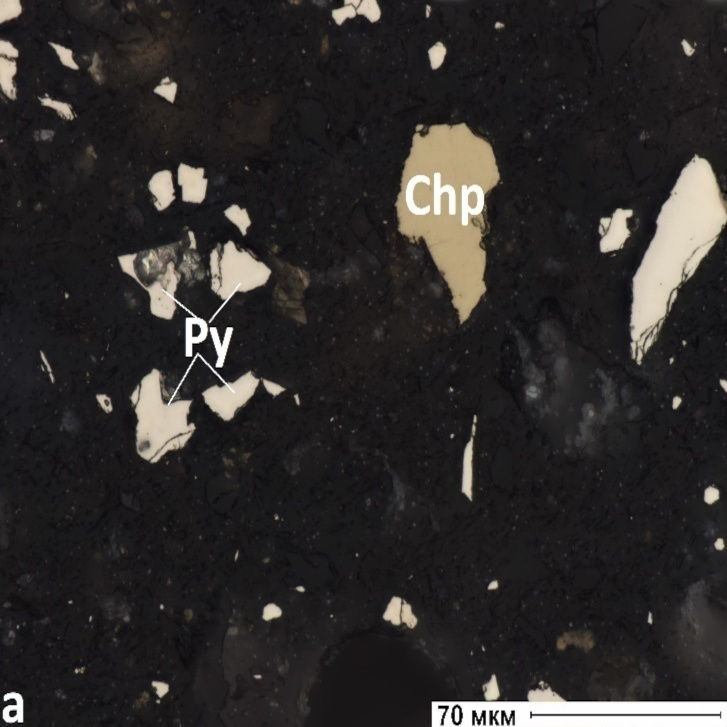
\includegraphics[width=0.8\textwidth]{assets/296}
% 	\caption*{}
% \end{figure}
% \end{minipage} & \begin{minipage}[b]{\linewidth}\raggedright
% \begin{figure}[H]
% 	\centering
% 	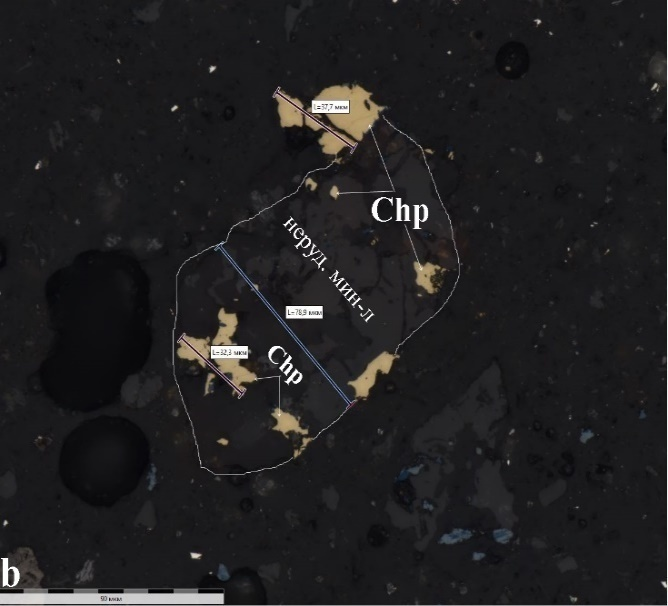
\includegraphics[width=0.8\textwidth]{assets/297}
% 	\caption*{}
% \end{figure}
% \end{minipage} \\
% \midrule\noalign{}
% \endhead
% \bottomrule\noalign{}
% \endlastfoot
% & \\
% \begin{figure}[H]
% 	\centering
% 	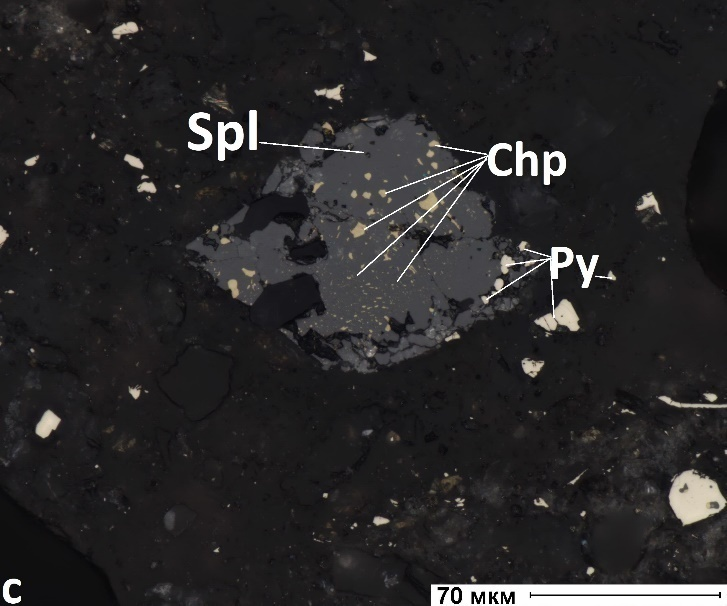
\includegraphics[width=0.8\textwidth]{assets/298}
% 	\caption*{}
% \end{figure} &
% \begin{figure}[H]
% 	\centering
% 	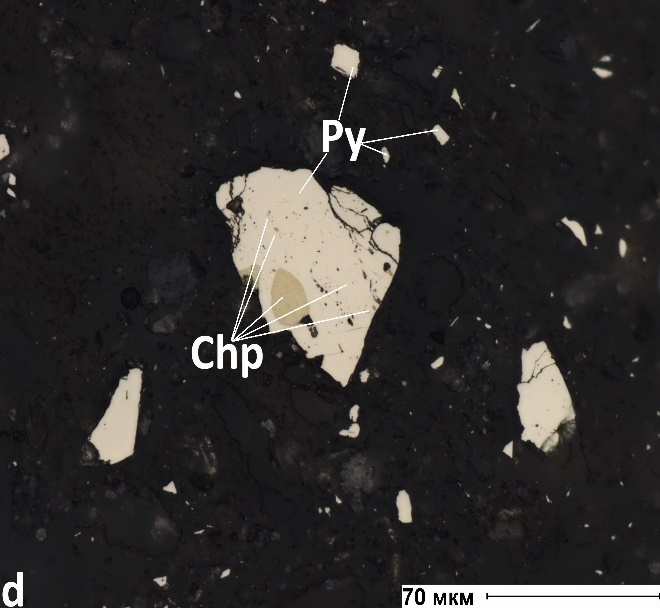
\includegraphics[width=0.8\textwidth]{assets/299}
% 	\caption*{}
% \end{figure} \\
% \multicolumn{2}{@{}>{\raggedright\arraybackslash}p{(\columnwidth - 2\tabcolsep) * \real{1.0000} + 2\tabcolsep}@{}}{%
% Chp-халькопирит, Spl-сфалерит, Py-пирит.
% 
% {\bfseries Рис. 1 -- Характеристика выделений халькопирита. Увел.
% 200/500}} \\
% \end{longtable}

Проведены исследования с использованием сверхтонкого измельчения в
лабораторной бисерной мельнице (далее МБЛ-1) по определению кинетики
измельчения исходной пробы отвальных хвостов контролем крупности
исходного продукта.

Известно, что использование тонкого и сверхтонкого помола продуктов,
содержащих благородные металлы, значительно увеличивает извлечение
золота и серебра в процессе обогащения. Но возможность моделирования
процесса измельчения в непрерывном режиме для бисерной мельницы является
основной проблемой на данный момент.

На рынке лабораторного оборудования представлен широкий ассортимент
лабораторных бисерных мельниц, зарубежных компании, среди разработок в
России -- это мельница МПБ -- 1 совместного российского-казахстанского
производства ТОО «SMAK Technology» и ООО БФК «Инжиниринг».

Лаборатории ООО "БФК Инжиниринг" и полупромышленные бисерные мельницы
имеют возможность моделировать технологический процесс ультратонкого
измельчения в поточном режиме {[}13{]}.

Внешний вид мельницы показаны на рисунке 2.

\begin{figure}[H]
	\centering
	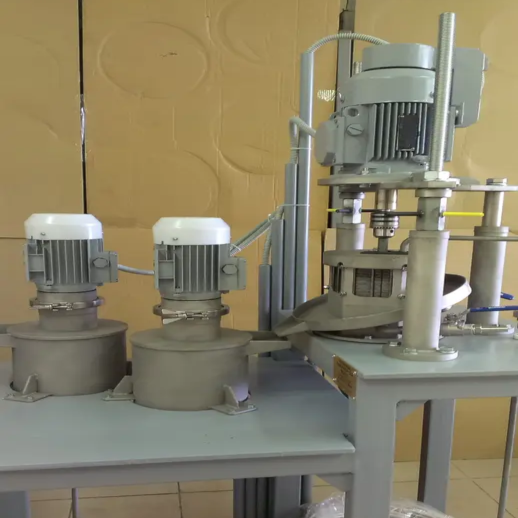
\includegraphics[width=0.8\textwidth]{assets/300}
	\caption*{}
\end{figure}

{\bfseries Рис. 2 -- Внешний вид бисерной мельницы МБЛ -- 1 для
сверхтонкого измельчения}

Флотационное обогащение выполнялось на стандартных лабораторных
пневмомеханических флотационных машинах типа Вэктис с объемом камер 3,
1.0 и 0.5 л.

Для исследования были применены следующие реагенты:

- сернистый натрий -- активатор;

- ксантогенат бутиловый - собиратель;

- МИБК -- пенообразователь;

Из вышеперечисленных реагентов приготавливались растворы необходимой
концентрации, с пересчетом на 100 \% активность, по формуле:

\[Р = \frac{V \bullet C}{A};\]

где V -- объем воды, мл; А -- активность, \%; C -- концентрация
реагента, д.е;

{\bfseries Результаты и обсуждение.} Результаты определения кинетики
измельчения исходной пробы хвостов c контролем крупности исходного
продукта представлены в таблице 1.

{\bfseries Таблица 1 -- Кинетика измельчения отвальных хвостов обогащения}

\begin{longtable}[]{@{}
  >{\raggedright\arraybackslash}p{(\columnwidth - 22\tabcolsep) * \real{0.1875}}
  >{\raggedright\arraybackslash}p{(\columnwidth - 22\tabcolsep) * \real{0.1031}}
  >{\raggedright\arraybackslash}p{(\columnwidth - 22\tabcolsep) * \real{0.0620}}
  >{\raggedright\arraybackslash}p{(\columnwidth - 22\tabcolsep) * \real{0.0732}}
  >{\raggedright\arraybackslash}p{(\columnwidth - 22\tabcolsep) * \real{0.0732}}
  >{\raggedright\arraybackslash}p{(\columnwidth - 22\tabcolsep) * \real{0.0620}}
  >{\raggedright\arraybackslash}p{(\columnwidth - 22\tabcolsep) * \real{0.0732}}
  >{\raggedright\arraybackslash}p{(\columnwidth - 22\tabcolsep) * \real{0.0732}}
  >{\raggedright\arraybackslash}p{(\columnwidth - 22\tabcolsep) * \real{0.0732}}
  >{\raggedright\arraybackslash}p{(\columnwidth - 22\tabcolsep) * \real{0.0732}}
  >{\raggedright\arraybackslash}p{(\columnwidth - 22\tabcolsep) * \real{0.0732}}
  >{\raggedright\arraybackslash}p{(\columnwidth - 22\tabcolsep) * \real{0.0732}}@{}}
\toprule\noalign{}
\multirow{2}{=}{\begin{minipage}[b]{\linewidth}\raggedright
Наименование продуктов, мм
\end{minipage}} &
\multirow{2}{=}{\begin{minipage}[b]{\linewidth}\raggedright
Выход, \%
\end{minipage}} &
\multicolumn{5}{>{\raggedright\arraybackslash}p{(\columnwidth - 22\tabcolsep) * \real{0.3436} + 8\tabcolsep}}{%
\begin{minipage}[b]{\linewidth}\raggedright
Содержание, \%
\end{minipage}} &
\multicolumn{5}{>{\raggedright\arraybackslash}p{(\columnwidth - 22\tabcolsep) * \real{0.3658} + 8\tabcolsep}@{}}{%
\begin{minipage}[b]{\linewidth}\raggedright
Распределение, \%
\end{minipage}} \\
& & \begin{minipage}[b]{\linewidth}\raggedright
Cu
\end{minipage} & \begin{minipage}[b]{\linewidth}\raggedright
Fe
\end{minipage} & \begin{minipage}[b]{\linewidth}\raggedright
S
\end{minipage} & \begin{minipage}[b]{\linewidth}\raggedright
Au
\end{minipage} & \begin{minipage}[b]{\linewidth}\raggedright
Ag
\end{minipage} & \begin{minipage}[b]{\linewidth}\raggedright
Cu
\end{minipage} & \begin{minipage}[b]{\linewidth}\raggedright
Fe
\end{minipage} & \begin{minipage}[b]{\linewidth}\raggedright
S
\end{minipage} & \begin{minipage}[b]{\linewidth}\raggedright
Au
\end{minipage} & \begin{minipage}[b]{\linewidth}\raggedright
Ag
\end{minipage} \\
\midrule\noalign{}
\endhead
\bottomrule\noalign{}
\endlastfoot
\multicolumn{12}{@{}>{\raggedright\arraybackslash}p{(\columnwidth - 22\tabcolsep) * \real{1.0000} + 22\tabcolsep}@{}}{%
Исходная проба} \\
+0,071 & 16,91 & 0,17 & 5,39 & 2,05 & 0,37 & 2,66 & 12,48 & 7,39 & 3,11
& 8,01 & 5,54 \\
-0,071 + 0,045 & 14,34 & 0,18 & 11,65 & 10,75 & 0,56 & 5,67 & 11,12 &
13,55 & 13,81 & 10,23 & 10,03 \\
-0,045 + 0,035 & 12,07 & 0,22 & 17,69 & 16,73 & 1,20 & 9,35 & 11,33 &
17,32 & 18,09 & 18,61 & 13,91 \\
-0,035+0,025 & 11,32 & 0,26 & 20,34 & 19,47 & 1,15 & 10,83 & 12,58 &
18,67 & 19,75 & 16,73 & 15,12 \\
-0,025+0,017 & 6,47 & 0,15 & 16,18 & 14,71 & 0,95 & 6,98 & 4,29 & 8,49 &
8,53 & 7,90 & 5,57 \\
-0,017+0,008 & 10,52 & 0,15 & 16,71 & 14,88 & 0,98 & 8,63 & 6,89 & 14,26
& 14,03 & 13,21 & 11,19 \\
-0,008+0,006 & 1,25 & 0,15 & 15,49 & 10,89 & 0,99 & 7,53 & 0,82 & 1,57 &
1,22 & 1,59 & 1,16 \\
-0,006+0 & 27,12 & 0,34 & 8,53 & 8,83 & 0,68 & 11,21 & 40,49 & 18,75 &
21,46 & 23,72 & 37,48 \\
Исходная проба & 100,0 & 0,23 & 12,33 & 11,16 & 0,78 & 8,11 & 100,0 &
100,0 & 100,0 & 100,0 & 100,0 \\
\multicolumn{12}{@{}>{\raggedright\arraybackslash}p{(\columnwidth - 22\tabcolsep) * \real{1.0000} + 22\tabcolsep}@{}}{%
Время измельчения 5 мин} \\
+0,071 & 10,61 & 0,21 & 4,87 & 3,08 & 0,28 & 3,2 & 9,76 & 4,19 & 2,93 &
3,81 & 4,18 \\
-0,071 + 0,045 & 3,14 & 0,47 & 28,11 & 30,14 & 1,76 & 18,34 & 6,47 &
7,16 & 8,48 & 7,09 & 7,10 \\
-0,045 + 0,035 & 12,01 & 0,13 & 15,27 & 14,62 & 1,02 & 9,14 & 6,96 &
14,87 & 15,73 & 15,75 & 13,53 \\
-0,035+0,025 & 20,70 & 0,2 & 13,43 & 12,7 & 0,8 & 7,71 & 17,56 & 22,54 &
23,56 & 21,11 & 19,68 \\
-0,025+0,017 & 5,47 & 0,17 & 12,44 & 11,34 & 0,75 & 7,32 & 4,07 & 5,52 &
5,56 & 5,28 & 4,94 \\
-0,017+0,008 & 10,60 & 0,16 & 11,29 & 10,01 & 0,7 & 6,2 & 7,22 & 9,71 &
9,51 & 9,46 & 8,11 \\
-0,008+0,006 & 0,49 & 0,16 & 10,06 & 7,98 & 0,73 & 5,47 & 0,34 & 0,40 &
0,35 & 0,46 & 0,33 \\
-0,006+0 & 36,98 & 0,3 & 11,87 & 10,22 & 0,78 & 9,24 & 47,62 & 35,61 &
33,88 & 37,04 & 42,13 \\
Исходная проба & 100,0 & 0,23 & 12,33 & 11,16 & 0,78 & 8,11 & 100,0 &
100,0 & 100,0 & 100,0 & 100,0 \\
\multicolumn{12}{@{}>{\raggedright\arraybackslash}p{(\columnwidth - 22\tabcolsep) * \real{1.0000} + 22\tabcolsep}@{}}{%
Время измельчения 10 мин} \\
+0,071 & 8,60 & 0,22 & 3,64 & 1,78 & 0,35 & 2,08 & 8,10 & 2,54 & 1,37 &
3,81 & 2,21 \\
-0,071 + 0,045 & 2,74 & 0,35 & 20,2 & 20,69 & 2,02 & 12,11 & 4,11 & 4,49
& 5,08 & 7,09 & 4,09 \\
-0,045 + 0,035 & 5,97 & 0,24 & 15,26 & 14,48 & 2,06 & 8,24 & 6,26 & 7,38
& 7,74 & 15,75 & 6,06 \\
-0,035+0,025 & 15,37 & 0,21 & 14,98 & 14,61 & 1,07 & 8,72 & 14,35 &
18,67 & 20,13 & 21,11 & 16,52 \\
-0,025+0,017 & 4,82 & 0,21 & 14,79 & 14,24 & 0,86 & 8,16 & 4,34 & 5,78 &
6,15 & 5,28 & 4,85 \\
-0,017+0,008 & 11,42 & 0,17 & 13,15 & 12,28 & 0,65 & 7,39 & 8,60 & 12,18
& 12,56 & 9,46 & 10,40 \\
-0,008+0,006 & 0,52 & 0,19 & 11,99 & 10,85 & 0,69 & 6,96 & 0,42 & 0,51 &
0,51 & 0,46 & 0,45 \\
-0,006+0 & 50,56 & 0,24 & 11,81 & 10,25 & 0,57 & 8,89 & 53,82 & 48,45 &
46,46 & 37,04 & 55,42 \\
Исходная проба & 100,0 & 0,23 & 12,33 & 11,16 & 0,78 & 8,11 & 100,0 &
100,0 & 100,0 & 100,0 & 100,0 \\
\multicolumn{12}{@{}>{\raggedright\arraybackslash}p{(\columnwidth - 22\tabcolsep) * \real{1.0000} + 22\tabcolsep}@{}}{%
Время измельчения 20 мин} \\
+0,071 & 5,33 & 0,20 & 3,71 & 1,89 & 0,25 & 2,03 & 4,52 & 1,60 & 0,90 &
1,70 & 1,33 \\
-0,071 + 0,045 & 3,07 & 0,37 & 22,43 & 23,69 & 1,52 & 13,17 & 4,90 &
5,58 & 6,51 & 5,97 & 4,98 \\
-0,045 + 0,035 & 3,58 & 0,25 & 15,83 & 15,64 & 0,99 & 9,14 & 3,95 & 4,59
& 5,01 & 4,55 & 4,03 \\
-0,035+0,025 & 10,02 & 0,21 & 14,78 & 14,45 & 0,97 & 7,93 & 9,12 & 12,01
& 12,97 & 12,47 & 9,80 \\
-0,025+0,017 & 3,67 & 0,19 & 14,19 & 13,61 & 0,95 & 7,67 & 3,03 & 4,22 &
4,47 & 4,45 & 3,47 \\
-0,017+0,008 & 9,10 & 0,16 & 12,65 & 11,65 & 0,84 & 6,63 & 6,53 & 9,34 &
9,50 & 9,82 & 7,44 \\
-0,008+0,006 & 0,63 & 0,22 & 12,06 & 10,75 & 0,81 & 6,66 & 0,61 & 0,62 &
0,61 & 0,65 & 0,52 \\
-0,006+0 & 64,62 & 0,24 & 11,84 & 10,37 & 0,73 & 8,59 & 67,34 & 62,03 &
60,03 & 60,39 & 68,42 \\
Исходная проба & 100,0 & 0,23 & 12,33 & 11,16 & 0,78 & 8,11 & 100,0 &
100,0 & 100,0 & 100,0 & 100,0 \\
\end{longtable}

Зависимость выхода класса крупности минус 0,006 мм от времени
ультратонкого измельчения показан на рисунке 3.

{\bfseries Рис. 3 -- Зависимость выхода класса -0,006 мм от времени
измельчения}

Анализ ситовых характеристик хвостов после ультратонкого измельчения
показывает, что наибольшая концентрация меди приходится на самый тонкий
класс -0,006+0 мм, и повышается в зависимости от времени измельчения с
47,62 \% (5 минут) до 67.34 \% (20 минут), что свидетельствует о высоком
раскрытии медных минералов за счет ультратонкого измельчения. Однако,
увеличение выхода тонкого класса -0,006+0 мм с 27,12 \% в исходных
хвостах (см. таблицу 1) до 64,42 \% может отрицательно сказываться на
показателях обогащения, за счет ошламования процесса.

Кроме того, в тонких классах вместе с медью концентрируется и железо,
что подтверждает тесную связь минералов меди с пиритом, которую не
удается разрушить даже при ультратонком измельчении.

С целью определения влияния степени ультратонкого измельчения на
извлечение меди и благородных металлов выполнены флотационные тесты.

Схема проведения опыта указана на рисунке 4. Условия опытов приведены в
таблице 2; результаты представлены на рисунке 5-7.

Концентрат 2

Хвосты

Основная Cu флотация

УТИ

Исходная проба

Контрольная флотация

Концентрат 2

{\bfseries Рис. 4 -- Лабораторная схема проведения опыта}

{\bfseries Таблица 2 -- Условия проведения опыта}

\begin{longtable}[]{@{}
  >{\raggedright\arraybackslash}p{(\columnwidth - 16\tabcolsep) * \real{0.2981}}
  >{\raggedright\arraybackslash}p{(\columnwidth - 16\tabcolsep) * \real{0.1195}}
  >{\raggedright\arraybackslash}p{(\columnwidth - 16\tabcolsep) * \real{0.0685}}
  >{\raggedright\arraybackslash}p{(\columnwidth - 16\tabcolsep) * \real{0.0963}}
  >{\raggedright\arraybackslash}p{(\columnwidth - 16\tabcolsep) * \real{0.0990}}
  >{\raggedright\arraybackslash}p{(\columnwidth - 16\tabcolsep) * \real{0.0946}}
  >{\raggedright\arraybackslash}p{(\columnwidth - 16\tabcolsep) * \real{0.0597}}
  >{\raggedright\arraybackslash}p{(\columnwidth - 16\tabcolsep) * \real{0.0747}}
  >{\raggedright\arraybackslash}p{(\columnwidth - 16\tabcolsep) * \real{0.0896}}@{}}
\toprule\noalign{}
\multirow{2}{=}{\begin{minipage}[b]{\linewidth}\raggedright
Операция
\end{minipage}} &
\multirow{2}{=}{\begin{minipage}[b]{\linewidth}\raggedright
Время,

мин
\end{minipage}} &
\multirow{2}{=}{\begin{minipage}[b]{\linewidth}\raggedright
рН
\end{minipage}} &
\multicolumn{5}{>{\raggedright\arraybackslash}p{(\columnwidth - 16\tabcolsep) * \real{0.4243} + 8\tabcolsep}}{%
\begin{minipage}[b]{\linewidth}\raggedright
Расход реагентов, г/т
\end{minipage}} & \begin{minipage}[b]{\linewidth}\raggedright
\end{minipage} \\
& & & \begin{minipage}[b]{\linewidth}\raggedright
МБС
\end{minipage} & \begin{minipage}[b]{\linewidth}\raggedright
Na\textsubscript{2}S
\end{minipage} & \begin{minipage}[b]{\linewidth}\raggedright
H\textsubscript{2}SO\textsubscript{4}
\end{minipage} & \begin{minipage}[b]{\linewidth}\raggedright
Кх
\end{minipage} & \begin{minipage}[b]{\linewidth}\raggedright
Aero 3418
\end{minipage} & \begin{minipage}[b]{\linewidth}\raggedright
МИБК
\end{minipage} \\
\begin{minipage}[b]{\linewidth}\raggedright
{\bfseries Всего:}
\end{minipage} & \begin{minipage}[b]{\linewidth}\raggedright
{\bfseries -}
\end{minipage} & \begin{minipage}[b]{\linewidth}\raggedright
{\bfseries -}
\end{minipage} & \begin{minipage}[b]{\linewidth}\raggedright
{\bfseries 800}
\end{minipage} & \begin{minipage}[b]{\linewidth}\raggedright
{\bfseries 150}
\end{minipage} & \begin{minipage}[b]{\linewidth}\raggedright
{\bfseries 7000}
\end{minipage} & \begin{minipage}[b]{\linewidth}\raggedright
{\bfseries 100}
\end{minipage} & \begin{minipage}[b]{\linewidth}\raggedright
{\bfseries 15}
\end{minipage} & \begin{minipage}[b]{\linewidth}\raggedright
{\bfseries 10}
\end{minipage} \\
\begin{minipage}[b]{\linewidth}\raggedright
Измельчение, -0,045 мм
\end{minipage} & \begin{minipage}[b]{\linewidth}\raggedright
5,10,20
\end{minipage} & \begin{minipage}[b]{\linewidth}\raggedright
-
\end{minipage} & \begin{minipage}[b]{\linewidth}\raggedright
800
\end{minipage} & \begin{minipage}[b]{\linewidth}\raggedright
-
\end{minipage} & \begin{minipage}[b]{\linewidth}\raggedright
-
\end{minipage} & \begin{minipage}[b]{\linewidth}\raggedright
-
\end{minipage} & \begin{minipage}[b]{\linewidth}\raggedright
-
\end{minipage} & \begin{minipage}[b]{\linewidth}\raggedright
-
\end{minipage} \\
\midrule\noalign{}
\endhead
\bottomrule\noalign{}
\endlastfoot
Основная Cu флотация & 10 & 7,7 & - & 150 & - & - & 15 & 5 \\
Контрольная флотация & 10 & 3,0 & - & - & 7000 & 100 & - & 5 \\
\end{longtable}

{\bfseries Рис. -- 5. Результаты тестов по подбору степени измельчения для
медных минералов}

{\bfseries Рис.-- 6. Зависимость извлечения золота от степени измельчения
отвальных хвостов обогащения}

{\bfseries Рис. -- 7. Зависимость извлечения серебра от степени измельчения
отвальных хвостов обогащения}

Из рисунков 5-7 следует, что с увеличением тонины помола по классу
крупности -0,045+0 мм с 69 до 86 \% наблюдается повышение извлечения
меди в суммарном концентрате на 7,03 \% (66,49 до 73,52 \%), также
повышается извлечения благородных металлов, золота на 6,71 \% (71,07 до
77,78 \%), серебро на 6,42 \% (70,29 \% до 76,71 \%).

{\bfseries Выводы.} Для расширения сырьевой базы и комплексного
использования сырья Казахстана принято решение о необходимости
рассмотрении возможности вторичной переработки отвальных хвостов
Карагайлинской обогатительной фабрики, за складированных в карьере
«Главный».

Выделение ценных компонентов из мелкозернистых руд часто достигается
только после того, как размер частицы руды снижается до уровня ниже
порового значения традиционной шаровой мельницы в - 0,045 мм.

Проведены исследования с использованием сверхтонкого измельчения в
лабораторной бисерной мельнице (далее МБЛ-1) по определению кинетики
измельчения исходной пробы отвальных хвостов контролем крупности
исходного продукта.

Чтобы определить влияние степени сверхтонкого измельчения на извлечение
меди и благородных металлов, были проведены флотационные тесты.

Из результатов представленный в графике 5-7 следует, что оптимальный
тонины помола по классу крупности -- 0,045 +0 мм 86 \%, при это
наблюдается увлечения извлечения меди в суммарной концентрат на 73,52
\%, золота на 77,78 \%, серебро на 76,71 \%.

{\bfseries Литература}

\begin{enumerate}
\def\labelenumi{\arabic{enumi}.}
\item
  Xin Fang, Caibin Wu, Ningning Liao, Chengfang Yuan, Bin Xie, Jiaqi
  Tong. The first attempt of applying ceramic balls in industrial
  tumbling mill: A case study // Minerals Engineering. 2022. Volume 180.
  DOI: 10.1016/j.mineng.2022.107504
\item
  Jean-Paul Duroudier Size Reduction of Divided Solids // 2 - Grinding
  Energy. - 2016. -P. 53-72.
\item
  Paul Hassall, Emmanuel Nonnet,Ville Keikkala, Tarja Komminaho, Liisa
  Kotila. Ceramic bead behavior in ultra-fine grinding mills // Minerals
  Engineering. -2016. --Vol. 98. -P. 232-239.
\item
  Xin Fang, Caibin Wu, Ningning Liao, Chengfang Yuan, Bin Xie, Jiaqi
  Tong. The first attempt of applying ceramic balls in industrial
  tumbling mill: A case study // Minerals Engineering. -2022. --Vol.
  180. DOI: 10.1016/j.mineng.2022.107504
\item
  Song Z.G., Corin K.C., Wiese J.G., O\textquotesingle Connor C.T.
  Effect of different grinding media composition on the flotation of a
  PGM ore // Minerals Engineering. -2018. --Vol. 124. -P. 74-76.
  DOI:10.1016/j.mineng.2018.05.014
\item
  Xiaolong Zhang, Yuexin Han, Yanjun Li, Wenbo Li, Jiancheng He,
  Jianping Jin Strengthening the flotation recovery of silver using a
  special ceramic-medium stirred mill // Powder Technology. -2022.
  --Vol. 406. DOI: 10.1016/j.powtec.2022.117585
\item
  Caibin, W., Kuangdi, X. Ultrafine Grinding Process. In: Xu, K. (eds)
  The ECPH Encyclopedia of Mining and Metallurgy. -Springer, Singapore,
  2023. DOI: 10.1007/978-981-19-0740-1
\item
  Tuokuu F.X., Kpinpuo S.D., Hinson R.E. Sustainable development in
  Ghana\textquotesingle s gold mines: clarifying the
  stakeholder\textquotesingle s perspective // Journal of Sustainable
  Mining. -- 2019. -- Vol. 18(2). 2019. -P. 77--84. DOI:
  10.1016/j.jsm.2019.02.007
\item
  Borujeni M.P., Gitinavard H., Evaluating the sustainable mining
  contractor selection problems: An imprecise last aggregation
  preference selection index method // Journal of Sustainable Mining. --
  2017. -- Vol. 16(4). 2017 pp 207--218. DOI: 10.1016/J.JSM.2017.12.006
\item
  Pier Paolo Manca, Giorgio Massacci, Davide Pintus, Giulio Sogos. The
  flotation of sphalerite mine tailings as a remediation method//
  Minerals Engineering. -2021. - Vol. 165. DOI:
  10.1016/j.mineng.2021.106862
\item
  Kasongo K.B., Mwanat M. H., Ngamba Guellord , Merveille Kimpiab , K.
  Fabrice Kapiamba. Statistical investigation of flotation parameters
  for copper recovery from sulfide flotation tailings. // Results in
  Engineering. -2021. --Vol. 9. DOI: 10.1016/j.rineng.2021.100207
\item
  Malte Drobe, Frank Haubrich, Mariano Gajardo and Herwig Marbler.
  Processing Tests, Adjusted Cost Models and the Economies
  ofReprocessing Copper Mine Tailings in Chile. // Metals 2021. -Vol.
  11. - P. 1031-1052. DOI:10.3390/met11010103
\item
  Сидоров И.А., Войлошников Г.И., Рубцов П.Н., Бондарь В.В., Грицай С.Г.
  Испытания мельницы производства ООО «БФК Инжиниринг» для ультратонкого
  измельчения упорных золотосодержащих сульфидных концентратов // Горный
  информационно -- аналитический бюллетень (научно-технический журнал).
  -2015. - С. 161 -- 166.
\end{enumerate}

{\bfseries References}

\begin{enumerate}
\def\labelenumi{\arabic{enumi}.}
\item
  Xin Fang, Caibin Wu, Ningning Liao, Chengfang Yuan, Bin Xie, Jiaqi
  Tong. The first attempt of applying ceramic balls in industrial
  tumbling mill: A case study // Minerals Engineering. 2022. Volume 180.
  DOI: 10.1016/j.mineng.2022.107504
\item
  Jean-Paul Duroudier Size Reduction of Divided Solids // 2 - Grinding
  Energy. - 2016. -P. 53-72.
\item
  Paul Hassall, Emmanuel Nonnet,Ville Keikkala, Tarja Komminaho, Liisa
  Kotila. Ceramic bead behavior in ultra-fine grinding mills // Minerals
  Engineering. -2016. --Vol. 98. -P. 232-239.
\item
  Xin Fang, Caibin Wu, Ningning Liao, Chengfang Yuan, Bin Xie, Jiaqi
  Tong. The first attempt of applying ceramic balls in industrial
  tumbling mill: A case study // Minerals Engineering. -2022. --Vol.
  180. DOI: 10.1016/j.mineng.2022.107504
\item
  Song Z.G., Corin K.C., Wiese J.G., O\textquotesingle Connor C.T.
  Effect of different grinding media composition on the flotation of a
  PGM ore // Minerals Engineering. -2018. --Vol. 124. -P. 74-76.
  DOI:10.1016/j.mineng.2018.05.014
\item
  Xiaolong Zhang, Yuexin Han, Yanjun Li, Wenbo Li, Jiancheng He,
  Jianping Jin Strengthening the flotation recovery of silver using a
  special ceramic-medium stirred mill // Powder Technology. -2022.
  --Vol. 406. DOI: 10.1016/j.powtec.2022.117585
\item
  Caibin, W., Kuangdi, X. Ultrafine Grinding Process. In: Xu, K. (eds)
  The ECPH Encyclopedia of Mining and Metallurgy. -Springer, Singapore,
  2023. DOI: 10.1007/978-981-19-0740-1
\item
  Tuokuu F.X., Kpinpuo S.D., Hinson R.E. Sustainable development in
  Ghana\textquotesingle s gold mines: clarifying the
  stakeholder\textquotesingle s perspective // Journal of Sustainable
  Mining. -- 2019. -- Vol. 18(2). 2019. -P. 77--84. DOI:
  10.1016/j.jsm.2019.02.007
\item
  Borujeni M.P., Gitinavard H., Evaluating the sustainable mining
  contractor selection problems: An imprecise last aggregation
  preference selection index method // Journal of Sustainable Mining. --
  2017. -- Vol. 16(4). 2017 pp 207--218. DOI: 10.1016/J.JSM.2017.12.006
\item
  Pier Paolo Manca, Giorgio Massacci, Davide Pintus, Giulio Sogos. The
  flotation of sphalerite mine tailings as a remediation method//
  Minerals Engineering. -2021. - Vol. 165. DOI:
  10.1016/j.mineng.2021.106862
\item
  Kasongo K.B., Mwanat M. H., Ngamba Guellord , Merveille Kimpiab , K.
  Fabrice Kapiamba. Statistical investigation of flotation parameters
  for copper recovery from sulfide flotation tailings. // Results in
  Engineering. -2021. --Vol. 9. DOI: 10.1016/j.rineng.2021.100207
\item
  Malte Drobe, Frank Haubrich, Mariano Gajardo and Herwig Marbler.
  Processing Tests, Adjusted Cost Models and the Economies
  ofReprocessing Copper Mine Tailings in Chile. // Metals 2021. -Vol.
  11. - P. 1031-1052. DOI:10.3390/met11010103
\end{enumerate}

13. Sidorov I.A., Voiloshnikov G.I., Rubtsov P.N.,
Bondar\textquotesingle{} V.V., Gritsai S.G. Ispytaniya
mel\textquotesingle nitsy proizvodstva OOO «BFK Inzhiniring» dlya
ul\textquotesingle tratonkogo izmel\textquotesingle cheniya upornykh
zolotosoderzhashchikh sul\textquotesingle fidnykh kontsentratov //
Gornyi informatsionno -- analiticheskii byulleten\textquotesingle{}
(nauchno-tekhnicheskii zhurnal). -2015. - S. 161 -- 166. {[}in
Russian{]}

\emph{{\bfseries Сведения об авторах}}

Мамбеталиева А.Р. - доктор PhD, старший преподаватель кафедры
«Металлургии и обогащения полезных ископаемых» Satbayev University,
Алматы, Казахстан, e-mail: a.mambetaliyeva@satbayev.university;

Макашева Г.К. - докторант кафедры «Металлургии и обогащения полезных
ископаемых» Satbayev University, Алматы, Казахстан, e-mail:
mguldanka@mail.ru;

Тусупбекова Т.Ш. - докторант кафедры «Металлургии и обогащения полезных
ископаемых» Satbayev University, Алматы, Казахстан, e-mail:
tansholpan\_87.09@mail.ru;

Макашева Г.К. - докторант кафедры «Металлургии и обогащения полезных
ископаемых» Satbayev University, Алматы, Казахстан, e-mail:
mguldanka@mail.ru;

Калиаскаров С.К. - инженер-исследователь ТОО «КазГидроМедь», Караганда,
Казахстан, e-mail: sulya-95@mail.ru;

Сагатбек С. - магистр технических наук, инженер-исследователь ТОО
«КазГидроМедь», Караганда, Казахстан, e-mail: sunkar\_0396@mail.ru;

\emph{{\bfseries Information about the authors}}

Mambetaliyeva A.R. - PhD, Senior Lecturer at the Department of
Metallurgy and Mineral Processing at Satbayev University, Almaty,
Kazakhstan, e-mail: a.mambetaliyeva@satbayev.university;

Tusupbekova T.Sh. - doctoral student of the Department of Metallurgy and
Mineral Processing at Satbayev University, Almaty, Kazakhstan, e-mail:
tansholpan\_87.09@mail.ru;

Makasheva G. K., Doctoral student of the Department of Metallurgy and
Mineral Processing at Satbayev University, Almaty, Kazakhstan, e-mail:
mguldanka@mail.ru;

Kaliaskarov S.K.-Research Engineer at Kazhydromed LLP, Karaganda,
Kazakhstan, e-mail: sulya-95@mail.ru;

Sagatbek S. - Master of Technical Sciences, Research Engineer at
Kazhydromed LLP, Karaganda, Kazakhstan, e-mail: sunkar\_0396@mail.ru\newpage
{\bfseries ҒТАМР 52.01.93}

{\bfseries ТАУ-КЕН КӘСІПОРЫНДАРЫНЫҢ ЖҰМЫСКЕРЛЕРІНДЕ}

{\bfseries КӘСІПТІК АУРУЛАРДЫҢ ДАМУЫНЫҢ ӨНДІРІСТІК ҚАУІП ФАКТОРЛАРЫ}

{\bfseries А.М. Құрманов, А.М. Рахметова}\textsuperscript{🖂}, {\bfseries Э.А.
Құлмағамбетова,}

{\bfseries Н.Б. Әбдрахманова, Н.Т. Сағындықова}

Қазақстан Республикасы Еңбек және халықты әлеуметтік қорғау
министрлігінің

Еңбекті қорғау жөніндегі республикалық ғылыми-зерттеу институты ШЖҚ РМК,

Астана,Қазақстан

\textsuperscript{🖂}Корреспондент - автор: ra\_anar@mail.ru

Мақалада кәсіптік аурулардың даму факторы ретінде тау-кен кәсіпорны
қызметкерлерінің денсаулығына зиянды және қауіпті өндірістік
факторлардың әсер ету проблемасының қазіргі жағдайы қарастырылған.

Салыстыру топтары ретінде өндіріс қызметкерлері мен Қосалқы персонал
зерттелді, авторлар өндірістік объектілерді аттестаттау, сауалнама
деректерін талдады.

Еңбек қызметі процесінде зиянды және қауіпті өндірістік-кәсіптік
факторлардың тұрақты және қарқынды әсеріне ұшыраған қызметкерлердің
еңбек жағдайлары кәсіптік аурулардың жоғары таралуына және даму қаупінің
жоғарылауына ықпал ететіні анықталды. Өндіріс қызметкерлерінде кәсіптік
аурулардың даму қаупін төмендетудің кешенді тәсілі үшін
санитарлық-гигиеналық еңбек жағдайларын жақсарту, зиянды және қауіпті
өндірістік факторлардың әсерінен ұжымдық және жеке қорғаныс құралдарын
жетілдіру, алдын алу шараларын әзірлеу қажет.

{\bfseries Түйін сөздер:} тау-кен кәсіпорны, зиянды, қауіпті өндірістік
факторлар, кәсіптік тәуекел, кәсіптік аурулар.

{\bfseries ПРОИЗВОДСТВЕННЫЕ ФАКТОРЫ РИСКА РАЗВИТИЯ ПРОФЕССИОНАЛЬНЫХ
ЗАБОЛЕВАНИЙ У РАБОТНИКОВ ГОРНОДОБЫВАЮЩИХ ПРЕДПРИЯТИЙ}

{\bfseries А.М. Курманов, А.М. Рахметова}\textsuperscript{🖂}, {\bfseries Э.А.
Кульмагамбетова,}

{\bfseries Н.Б. Абдрахманова, Н.Т. Сагиндикова}

РГП на ПХВ Республиканский научно-исследовательский институт по охране
труда

Министерства труда и социальной защиты населения Республики Казахстан,

Астана, Казахстан,

e-mail: ra\_anar@mail.ru

В статье рассмотрено современное состояние проблемы влияния вредных и
опасных производственных факторов на здоровье работников
горнодобывающего предприятия, как фактор развития профессиональных
заболеваний.

В качестве групп сравнения обследованы работники производства и
вспомогательный персонал, авторами проанализированы данные аттестации
производственных объектов, анкетирования.

Установлено, что условия труда работников, подвергающихся в процессе
трудовой деятельности постоянному и интенсивному воздействию вредных и
опасных производственно-профессиональных факторов, способствуют более
высокой распространённости и более высокому риску развития
профессиональных заболеваний. Для комплексного подхода по снижению риска
развития профессиональных заболеваний у работников производства,
необходимо улучшение санитарно-гигиенических условий труда,
совершенствование средств коллективной и индивидуальной защиты от
воздействия вредных и опасных производственных факторов, разработка
превентивных мер профилактики.

{\bfseries Ключевые слова}: горнодобывающее предприятие, вредные, опасные
производственные факторы, профессиональный риск, профессиональные
заболевания.

{\bfseries OCCUPATIONAL RISK FACTORS FOR THE DEVELOPMENT OF OCCUPATIONAL
DISEASES IN MINING WORKERS}

{\bfseries A.M. Kurmanov, A.M. Rakhmetova}\textsuperscript{🖂}, {\bfseries E.A.
Kulmagambetova,}

{\bfseries N.B. Abdrakhmanova, N.T. Sagindykova}

RSE at the National Research Institute for Occupational Safety of the
Ministry of Labor

and Social Protection of the Population of the Republic of Kazakhstan,

Astana, Kazakhstan,

e-mail: ra\_anar@mail.ru

The article considers the current state of the problem of the influence
of harmful and dangerous production factors on the health of mining
enterprise workers as a factor in the development of occupational
diseases.

Production workers and support staff were examined as comparison groups,
the authors analyzed the data of certification of production facilities
and questionnaires.

It has been established that the working conditions of workers who are
exposed to constant and intense exposure to harmful and dangerous
occupational factors in the course of their work contribute to a higher
prevalence and a higher risk of developing occupational diseases. For an
integrated approach to reduce the risk of developing occupational
diseases in production workers, it is necessary to improve sanitary and
hygienic working conditions, improve collective and personal protection
against the effects of harmful and dangerous industrial factors, and
develop preventive preventive measures.

{\bfseries Key words}: mining enterprise, harmful, dangerous production
factors, occupational risk, occupational diseases.

{\bfseries Кіріспе.} Қазақстанның еңбекке қабілетті халқының денсаулығын
сақтау елдің табысты әлеуметтік-экономикалық дамуын қамтамасыз ету үшін
аса маңызды міндет болып табылады және Қазақстан Республикасының
2024-2030 жылдарға арналған Қауіпсіз еңбек тұжырымдамасында көрініс
табады {[}1{]}.

Қолайсыз өндірістік факторлар кешенінің тұрақты әсеріне ұшырайтын
тәуекел тобы тау-кен өнеркәсібінің жұмысшылары болып табылады {[}2,
3{]}.

Тау-кен өнеркәсібі ел экономикасында жетекші орындардың бірін алады және
зиянды, ауыр және қауіпті еңбек жағдайлары бар сала болып қала береді.

Өндірістік кәсіпорындардың жұмысшыларының денсаулық жағдайының
критерийлерінің бірі ретінде еңбекке қабілеттілігін уақытша жоғалтумен
сырқаттанушылықты зерттеу оның деңгейі мен нақты өндірістік фактілер
арасындағы байланысты орнатуға, сырқаттанушылықтың салдарынан
кәсіпорындардың экономикалық залалын анықтауға және оны төмендету
жөніндегі іс-шараларды әзірлеуге мүмкіндік береді {[}4{]}.

Шетелдік және отандық ғалымдардың пайымдауынша, өндірістік - шартты
ауруларды дамытудың кәсіптік тәуекел деңгейін анықтауда гигиеналық
критерийлер бойынша жұмысшылардың еңбек жағдайларын бағалау априори,
алдын-ала және сол арқылы болжамды болып табылады және оны денсаулық
жағдайының көрсеткіштері арқылы жұмысшылардың ағзасына қолайсыз кәсіптік
факторлардың әсер ету қаупін постериори, түпкілікті бағалау арқылы
күшейту керек. Бұл көрсеткіштерге кәсіби және кәсіби анықталған ауру,
сондай-ақ олардың негізінде есептелген интегралды көрсеткіштер жатады.

Авторлардың пікірінше {[}5-7{]}, тау-кен жұмысшыларының кәсіптік
ауруларының дамуына әсер ететін зиянды және қауіпті өндірістік факторлар
негізінен: шу, инфрақызыл, ауа ультрадыбысы; діріл (жалпы және
жергілікті), негізінен фиброгендік әсер ететін аэрозольдер, химиялық
фактор, еңбек процесінің ауырлығы мен шиеленісі. Тау-кен кәсіпорнында
осы факторлардың төмендеуі қазіргі кездегі өзекті мәселе екені сөзсіз.

Кәсіптік аурулар - дамуында жұмыс ортасы мен еңбек процесінің зиянды
және/немесе қауіпті факторларының әсерімен тікелей себеп-салдарлық
байланысты байқайтын аурулар {[}8{]}.

Кәсіптік аурудың даму мерзімі зиянды және/немесе қауіпті өндірістік
факторлар мен жұмыстардың әсер ету деңгейі мен ұзақтығына байланысты.
Бұрын оларды диагностикалау ұзақ уақыт бойы еңбек қызметі кезінде
аурудың сирек және спецификалық емес белгілері пайда болуымен қиындайды
{[}3, 8{]}.

Ресми статистиканың деректері жұмысшылардың еңбек жағдайлары мен кәсіби
денсаулығының қолайсыз жағдайын көрсетеді. Соңғы жылдары ҚР-дағы еңбек
гигиенасы және кәсіптік аурулар ұлттық орталығының мәліметтері бойынша
тау-кен өндіру кәсіпорындарында жұмыс істейтіндердің кәсіптік
сырқаттанушылығының салыстырмалы деңгейі өсуде, 2021 жылы 49,8\%,
2022-52,8\%, 2023-68\%. 2023 жылға арналған этиологиялық принцип бойынша
бастапқы кәсіптік аурулар топтары бойынша бөлу: өнеркәсіптік
аэрозольдердің әсерінен туындаған аурулар -35,4\%; жеке органдар мен
жүйелердің функционалдық шамадан тыс жүктелуіне және шамадан тыс
жүктелуіне байланысты аурулар -- 49,5\%, физикалық факторлардың әсеріне
байланысты аурулар -- 12,55; химиялық факторлардың әсерінен туындаған
аурулар -- 2,1\%.

Негізінен тірек-қимыл жүйесі (36,2\%), тыныс алу жүйесі (28,9\%) және
жүйке жүйесі (22,5\%) аурулары басым болды. Кәсіптік аурулардың ең көп
таралған үш нозологиялық түрі радикулопатия (32,1\%), созылмалы бронхит
(27,7\%) және моно-полиневропатия (15,4\%) болды {[}9{]}.

Тау-кен кәсіпорындарының өндірістік жағдайлары жұмыс аймағының ауасында
болатын зиянды химиялық элементтер кешенінің әсерімен сипатталады, бұл
жұмысшыларда патологиялық жағдайлардың, атап айтқанда тыныс алу
органдарының ауруларының дамуына әкелуі мүмкін. Жер асты тау - кен
жұмысшыларының кәсіби патологиясы тыныс алу жүйесі
ауруларының-пневмокониоздардың, жедел және созылмалы шаң бронхиттерінің
үлкен таралуымен сипатталады. Бұрғылау және жару жұмыстарын жүргізу
кезінде ұсақтау жұмыс аймағының ауасына (құрамында кремний диоксиді бар
бейорганикалық шаң) көп мөлшерде шаңның бөлінуі байқалады. Жұмыс
аймағының ауасында кездесетін негізгі заттардың арасында канцерогенді
заттар бар: никель, қорғасын, формальдегид, кадмий, бензин(а)пирен.
Күкірт ангидридінің, никельдің, азот оксидтерінің, акролеиннің,
формальдегидтің, кадмийдің, тоқтатылған заттардың тыныс алу органдарына
бір бағытты әсері байқалады. Марганец, қорғасын, селен жүйке жүйесіне
теріс әсер етуі мүмкін. Қан жүйесіне никель, қорғасын, көміртегі оксиді,
жүрек-тамыр жүйесіне - көміртегі оксиді мен селен теріс әсер етеді.
Жұмысшылардың еңбек жағдайлары тыныс алу жүйесінің кәсіби аурулары мен
қатерлі ісіктердің даму қаупін тудыратын жұмыс аймағының ауасындағы
химиялық заттардың қарқынды әсерімен сипатталады {[}10{]}.

Көптеген жылдар бойы тау-кен жұмысшыларының кәсіби ауруы, әсіресе, осы
зерттеудің мақсаты болып табылатын Тау-кен өнеркәсібіндегі маңызды
медициналық, әлеуметтік және экономикалық проблема болып қала береді.

Зерттеудің мақсаты тау-кен кәсіпорнының зиянды және қауіпті өндірістік
факторларының жұмысшылардың денсаулығына, кәсіптік аурулардың даму
қаупіне әсер ету ерекшеліктерін зерттеу болды.

{\bfseries Материалдар мен әдістер.} Өндірістік объектілерді аттестаттау
деректері зерттелді, өндіріс қызметкерлеріне сауалнама жүргізілді және
талданды. Салыстырудың екі тобы ретінде тау-кен кәсіпорнының өндірістік
және қосалқы қызметкерлерінің қызметкерлері зерттелді.

74 жұмысшының еңбек жағдайларына бағалау жүргізілді, оның ішінде жерасты
жұмыстарымен айналысатындар 67,6 \% (50 бірлік), автокөлік кәсіпорнында
- 18,2 \% (14 бірлік), ашық аумақтағы жұмыстар - 8,8 \% (6 бірлік) және
биіктіктегі жұмыстар - 5,4 \% (4 бірлік). Еңбек жағдайларын бағалау оның
ауырлығы мен шиеленісін, жұмыс орындарының микроклиматының
параметрлерін, физикалық және химиялық факторлардың әсер ету сипатын
ескере отырып жүргізілді.

Кен орнының негізгі аймағын өнеркәсіптік игеру 2023 жылғы 1 қаңтарда
басталды. Құрамында мыс, күміс, молибден және селен сияқты элементтер
бар кенді өндіру және байыту бойынша.

{\bfseries Нәтижелер және талқылау.} Кәсіпорындағы кәсіптік тәуекелдің
құрылымы мен дәрежесін талдау көптеген кәсіптердегі еңбек жағдайларын
зиянды деп бағалауға мүмкіндік берді, ал өткізгіштерде, жол
жұмысшыларында, бұрғылаушыларда, бұрғылаушылар мен жарылғыштардың
көмекшісінде-қауіпті (тау жыныстарының құлауы, тастар, құлау, үйінділер,
электр тогының соғуы, жарылыс, шаң).

Профилактикалық іс-шаралар кешенін жоспарлау кезінде еңбек жағдайларына
байланысты, оның ішінде осы өндіріс үшін Нақты химиялық фактордың
болуына байланысты аурулар тобын анықтаған жөн. Априорлық кәсіптік
тәуекелді сипаттайтын зияндылық пен қауіптің жоғары дәрежесі тау-кен
кәсіпорны қызметкерлерінің денсаулығы үшін кәсіптік қауіптің жоғары
деңгейін болжауға мүмкіндік береді.

Ақпаратқа сүйене отырып, жұмыс орындарын аттестациялау деректерінің
талдауынан өндірістік орта жұмысшыларға теріс әсер ететін химиялық
факторлар кешенінің болуымен сипатталады (1-кесте).

{\bfseries 1-кесте. Жұмысшылардың денсаулығына әсер ететін химиялық
факторлар тізімі}

\begin{longtable}[]{@{}
  >{\raggedright\arraybackslash}p{(\columnwidth - 6\tabcolsep) * \real{0.0583}}
  >{\raggedright\arraybackslash}p{(\columnwidth - 6\tabcolsep) * \real{0.3237}}
  >{\raggedright\arraybackslash}p{(\columnwidth - 6\tabcolsep) * \real{0.1177}}
  >{\raggedright\arraybackslash}p{(\columnwidth - 6\tabcolsep) * \real{0.5002}}@{}}
\toprule\noalign{}
\begin{minipage}[b]{\linewidth}\raggedright
п/п
\end{minipage} & \begin{minipage}[b]{\linewidth}\raggedright
Заттың атауы
\end{minipage} & \begin{minipage}[b]{\linewidth}\raggedright
Қауіптілік класы
\end{minipage} & \begin{minipage}[b]{\linewidth}\raggedright
Жұмысшы денсаулығына теріс әсері
\end{minipage} \\
\midrule\noalign{}
\endhead
\bottomrule\noalign{}
\endlastfoot
1 & Темір оксиді (II, III) & 3 & Сидероз (пневмокониоз) \\
2 & Марганец және оның қосылыстары & 2 & Аллергенді. мутагендік әсер \\
3 & Фторлы газ тәрізді қосылыстар & 2 & Қаңқа сүйектерінің қалыптасуы
мен өсуінің бұзылуы \\
4 & Хром (VI) оксиді /хром бойынша есептегенде & 1 & Демікпе, дерматит,
аллергиялық реакциялар, мутациялар \\
5 & Қалайы оксиді & 3 & Пневмокониоз \\
6 & Қорғасын және оның қосылыстары & 1 & Анемия, гипертензия, бүйрек
жеткіліксіздігі, иммундық және репродуктивті жүйеге уытты әсер \\
7 & Азот (IV)диоксиді & 2 & Өкпе ісінуі, жүйке аурулары \\
9 & Фторидтер нашар еритін бейорганикалық & 2 & Қаңқа сүйектерінің
қалыптасуы мен өсуінің бұзылуы \\
10 & Бейорганикалық шаң (кремний диоксиді) & 3 & Силикоз \\
11 & Диметилбензол & 3 & Жүрек-қан тамырлар органдарының созылмалы
зақымдануы, жүйке жүйесінің жұмысындағы бұзылулар, тері реакциялары,
астма \\
12 & Көміртек оксиді & 4 & Иммунологиялық белсенділіктің төмендеуі,
жоғарылауы қандағы қант мөлшері, жүрекке оттегінің берілуін
әлсіретеді. \\
13 & Метилбензол & 3 & Асма, химиялық бронхит, пневмония, өкпе ісінуі \\
14 & Бутан-1-ол & 3 & Көз ауруы (конъюнктивит, кератит), ОЖЖ \\
15 & Этанол & 4 & Онкологиялық, жүрек-қан тамырлары ауруы, эндокриндік
аурулар \\
16 & 2- этоксиэтанол (этил эфирі) & - & Бронхит, өкпенің қабынуы,
бронх-өкпе жүйесінің созылмалы аурулары, нейропсихикалық аурулар,
энцелофапатия, уытты гепатит және т. б. \\
17 & Бутил ацетат & 3 & Орталық жүйке жүйесі жүрек-тамыр жүйесі, бауыр,
бүйректің уытты құбылыстары \\
18 & Пропан-2-он (ацетон) & 4 & Тұншығу, мидағы тыныс алу орталығының
сал ауруы, мидың токсикалық ісінуі, өкпе ісінуі \\
19 & Уайт-спирит & - & Дерматит, экзема \\
20 & Көмірсутектер С\textsubscript{12}-С\textsubscript{19} & 4 & Тыныс
алу орталықтарының сал ауруы, орталық жүйке жүйесі \\
21 & Кальций дигидроксиді & 3 & Жоғарғы тыныс жолдарының тітіркенуі,
көздің, терінің, асқазан-ішек жолдарының зақымдалуы \\
22 & Күкірт диоксиді & 3 & В\textsubscript{1}, В\textsubscript{12}
дәрумендеріне жойқын әсер етеді. \\
23 & Күйе & 3 & Мутагендік және канцерогендік әсер \\
24 & Керосин & - & Күйік, улану. \\
\end{longtable}

1-кестенің деректері негізінде 4-қауіптілік класына мыналар жатады:
көмірсутектер С\textsubscript{12}-С\textsubscript{19}, пропан-2-он
(ацетон), этанол, көміртегі оксиді және т. б., олар жұмысшылардың
ағзасына уытты әсерімен сипатталады, иммунологиялық белсенділіктің
төмендеуіне, қандағы қант мөлшерінің жоғарылауына әкеледі, жүрекке
оттегінің берілуін әлсіретеді, онкологиялық, жүрек-тамыр жүйесі,
эндокриндік аурулар. Ұзақ уақыт әсер еткенде тұншығу, мидағы тыныс алу
орталығының параличі, мидың токсикалық ісінуі, өкпе ісінуі пайда болады.

Кестедегі мәліметтерге сәйкес 3-қауіптілік класына - темір оксиді,
қалайы оксиді, бейорганикалық шаң, диметилбензол, метилбензол, бутан,
бутил ацетаты, кальций дигидроксиді, күкірт диоксиді, күйе жатады. Бұл
химиялық заттар пневмокониоз, силикоз, сондай-ақ жүрек-қан тамырлар
органдарының созылмалы зақымдануы, жүйке жүйесінің бұзылуы, тері
реакциялары, астма, созылмалы бронхит, өкпе ісінуі және т. б. сияқты
кәсіби ауруларға әкеледі.

Зерттеу нәтижелерінің деректеріне сәйкес 2-қауіптілік класы мыналарды
сипаттайды: марганец және оның қосылыстары, фторлы қосылыстар,
аллергенді және мутагендік әсері бар азот диоксиді, қаңқа сүйектерінің
қалыптасуы мен өсуінің бұзылуын тудырады және т. б.

Осылайша, кәсіпорынның өндірістік жағдайлары жұмыс аймағының ауасында
болатын зиянды химиялық элементтер кешенінің әсерімен сипатталады, бұл
қызметкерлерде патологиялық жағдайлардың, кәсіптік аурулардың дамуына
әкелуі мүмкін.

Сауалнама деректерін талдау кезінде барлық бөлімшелерде жұмыс
істейтіндердің жас-еңбек өтілінің құрамы нақты айырмашылықтар болмағаны
және 35 жыл, ал көмекші персонал үшін-40,5 жыл болғандығы анықталды.
Өндірістік персонал үшін орташа жұмыс өтілі - 8,6 жыл, ал қосалқы
персонал үшін - 11 жыл болды (2-кесте).

2 кестеде жұмыс істейтіндерді мамандық бойынша бөлу көрсетілген

{\bfseries 2-кесте. Жұмысшыларды мамаңдық бойынша бөлу}

\begin{longtable}[]{@{}
  >{\raggedright\arraybackslash}p{(\columnwidth - 10\tabcolsep) * \real{0.0452}}
  >{\raggedright\arraybackslash}p{(\columnwidth - 10\tabcolsep) * \real{0.5249}}
  >{\raggedright\arraybackslash}p{(\columnwidth - 10\tabcolsep) * \real{0.1081}}
  >{\raggedright\arraybackslash}p{(\columnwidth - 10\tabcolsep) * \real{0.1167}}
  >{\raggedright\arraybackslash}p{(\columnwidth - 10\tabcolsep) * \real{0.1026}}
  >{\raggedright\arraybackslash}p{(\columnwidth - 10\tabcolsep) * \real{0.1025}}@{}}
\toprule\noalign{}
\multicolumn{6}{@{}>{\raggedright\arraybackslash}p{(\columnwidth - 10\tabcolsep) * \real{1.0000} + 10\tabcolsep}@{}}{%
\begin{minipage}[b]{\linewidth}\raggedright
Кәсіпорынның функционалдық құрылымы

(ауысымда жұмыс істейтіндердің жалпы саны -74)
\end{minipage}} \\
\midrule\noalign{}
\endhead
\bottomrule\noalign{}
\endlastfoot
\multicolumn{4}{@{}>{\raggedright\arraybackslash}p{(\columnwidth - 10\tabcolsep) * \real{0.7949} + 6\tabcolsep}}{%
Өндірістік персонал

(n=68)} &
\multicolumn{2}{>{\raggedright\arraybackslash}p{(\columnwidth - 10\tabcolsep) * \real{0.2051} + 2\tabcolsep}@{}}{%
Көмекші персонал

(n=6)} \\
№ & Мамандықтар & абс. & \% & абс. & \% \\
1 & Жол-сапар жұмысшысы (4) & 4 & 5,88 & & \\
2 & Сорғы қондырғыларының машинисі (4) & 4 & 5,88 & & \\
3 & Үңгуші (10) & 10 & 14,73 & & \\
4 & Тиеу-жеткізу машинасының машинисі (14) & 14 & 20,59 & & \\
5 & Бұрғылаушы (5) & 5 & 7,35 & & \\
6 & Бұрғылаушының көмекшісі (5) & 5 & 7,35 & & \\
7 & Электр дәнекерлеуші & 1 & 1,47 & & \\
8 & Электромонтер (2) & 2 & 2,94 & & \\
9 & Электрослесарь-монтажшы (2) & 2 & 2,94 & & \\
10 & Өздігінен жүретін жерасты машиналарының машинисі (2) & 2 & 2,94 &
& \\
11 & Өздігінен жүретін жерасты машиналарының машинисі көтергіш (2) & 2 &
2,94 & & \\
12 & Жанар-жағармай материалдарын жеткізу машинисі (2) & 2 & 2,94 & & \\
13 & Тау-кен жұмысшысы & 1 & 1,47 & & \\
14 & Жарылғыш материалдарды таратушы (2) & 2 & 2,94 & & \\
15 & Жерасты тау-кен жұмысшысы (жарылғыш материалдарды жеткізу бойынша)
(2) & 2 & 2,94 & & \\
16 & Ұсатқыш (1) & 1 & 1,47 & & \\
17 & Радиометрист - зертханашы (1) & 1 & 1,47 & & \\
18 & Маркшейдерлік жұмыстардағы тау-кен жұмысшысы (1) & 1 & 1,47 & & \\
19 & Жерасты өздігінен жүретін машинасының жүргізушісі & 1 & 1,47 & & \\
20 & Бас маркшейдер (1) & 1 & 1,47 & & \\
21 & Жарғыш (5) & 5 & 7,35 & & \\
22 & Тау шебері (1) & & & 1 & 6 \\
23 & Бас энергетик & & & 1 & 6 \\
24 & Энергетик & & & 1 & 6 \\
25 & Механик & & & 1 & 6 \\
26 & Учаске шебері (1) & & & 1 & 6 \\
27 & Бас механик (1) & & & 1 & 6 \\
\end{longtable}

2-кестенің деректері негізінде кәсіпорынның функционалдық құрылымы
үрлегіштерден (14,73), тиеу-жеткізу машинасының машинисінен (20,59\%),
бұрғылаушы мен бұрғылаушының көмекшісінен (тиісінше 7,35\%), жол-сапар
жұмысшысынан, сорғы қондырғыларының машинисінен (тиісінше 5,88\%),
электромонтерден, электр слесарь-монтаждаушыдан, өздігінен жүретін
жерасты машинисінен тұрады машиналарды көтергіш, жерасты өздігінен
жүретін машинасының жүргізушісі, жарылғыш материалдарды таратушы,
жерасты тау-кен жұмысшысы (тиісінше 2,94\% - дан), сондай-ақ тау-кен
жұмысшылары, маркшейдерлік жұмыстардағы тау-кен жұмысшылары, ұсатқыштар,
радиометрист зертханашы, жерасты өздігінен жүретін машинасының
жүргізушілері, негізгі маркшейдерлер мен жарылғыштар (сәйкесінше
1,47\%).

Жұмыс орындарындағы еңбек жағдайларын бағалау кезінде көбінесе
өндірістік орта факторларының аралас және аралас әсері байқалады,
сондықтан өндірістік персоналдың жұмысшылары басым зиянды өндірістік
факторларды ескере отырып, 6 топқа бөлінді.

1-ші топқа 3.3--3.4 еңбек жағдайларының сыныптарына сәйкес келетін
гигиеналық критерийлер бойынша жоғары кәсіби тәуекелі бар адамдар кірді:
үңгуші, тиеу-жеткізу машиналарының машинистері, бұрғылау қондырғысының
машинистері, экскаватор машинистері, тау-кен массасын жою машинистері,
ұсатқыштар.

Осы топтағы жұмысшылардың еңбек жағдайларының ерекшелігі зиянды және
қауіпті факторлар кешенінің бірлескен әсері болып табылады: аралас
діріл; шу (тұрақты емес), спектрде төмен және орташа жиілікті
компоненттер басым; дененің мәжбүрлі жағдайы, жүйке-бұлшықет кернеуі;
шаңның жоғарылауы; газдың жоғарылауы; қолайсыз микроклиматтық
жағдайларда жұмыс істеу; еңбек процесінің ауырлығы мен шиеленісі де
гигиеналық тұрғыдан маңызды. Еңбек ауырлығы перфораторларда, бұрғылау
қондырғыларында, тиеу - жеткізу машиналарында жұмыс істеуге байланысты,
еңбек процесінің шиеленісі ауысымда 12 сағатты құрайды.

Шаң факторы 20-дан 70\% - ға дейінгі шаңда (оның ішінде мыс, күміс,
селен, молибден және т.б.) SiO\textsubscript{2} құрамындағы негізінен
фиброгендік әсер ететін аэрозольдерден тұратын күрделі химиялық
құрамдағы шаңмен ұсынылған. Негізгі көздері бөлінетін зиянды газдар
болып табылады жару жұмыстары, жұмыс істейтін автокөлік, процестер
тотығу және жану пайдалы, сондай-ақ зиянды газдардың бөлінуін
жыныстардан және межпластовых суларды. Ішкі жану қозғалтқыштарының
жұмысына байланысты пайдаланылған газдардың жекелеген, неғұрлым
гигиеналық маңызды компоненттері шекті рұқсат етілген концентрациядан
асатын мөлшерде анықталады.

2-ші топқа ауыр жүк көліктерінің жүргізушілері, бульдозеристер кірді.
Еңбек жағдайлары аралас әсермен сипатталады: Жалпы және жергілікті діріл
(3.1--3.2 класс), тұрақты емес тербелмелі шу (3.1 класс), сенсорлық және
эмоционалдық жүктемелер орын алады, құрамында кремний диоксиді (кен) бар
Бейорганикалық шаңның және дизель отынының жану өнімдерінің газдарының
концентрациясы шекті рұқсат етілген концентрациядан аспайды.

3-ші топқа шаң, шу және қолайсыз микроклимат сияқты факторлардың басым
әсеріне ұшыраған жұмысшылар кірді. Бұл топтың жұмысшыларының арасында
гигиеналық критерийлер бойынша еңбек жағдайларының 3.1--3.3 сыныптарына
сәйкес келетін өте жоғары (тау-кен кенжарлары) немесе жоғары (жарылғыш
заттар, бекіткіштер) кәсіби тәуекелі бар кәсіби топтар бар.

4-ші топтың жұмысшылары үшін (сорғы қондырғысының машинистері, тау--кен
жабдықтарын жөндеу және техникалық қызмет көрсету слесарлары) физикалық
жүктеме мен дірілмен үйлескен технологиялық жабдықтың кең жолақты шуының
басым әсері тән (3.2-3.3 класс).

5-ші топты электр-газбен дәнекерлеушілер құрады, олардың еңбек
жағдайлары өндірістік факторлар кешенінің әсерімен сипатталады:
дәнекерлеу аэрозолының және негізінен фиброгендік әсер ететін
аэрозольдің құрамына кіретін марганец, темір, көміртек, азот
қосылыстары; қолайсыз микроклимат, физикалық шамадан тыс кернеу, шу.
Жұмыс аймағының ауасындағы марганец қосылыстарының құрамы 0,2
мг/м\textsuperscript{3} шекті рұқсат етілген концентрациядан кезінде
0,25 мг/м\textsuperscript{3} дейін құрайды (3.1-3.2 класс).

6-топ жұмысшылары үшін (электр дәнекерлеушілер мен электр слесарлары)
кернеуі 42 В және одан жоғары электр қондырғыларына қызмет көрсету және
жөндеу кезінде электромагниттік өрістер мен сәулеленулер, биіктікте
жұмыс істеу тән өндірістік факторлар болып табылады. Сонымен қатар,
жұмыс жабдықтың жұмыс режиміне жауапкершілікпен байланысты еңбек
процесінің жүйке-эмоционалды күйзелісімен сипатталады.

Осылайша, тау-кен өндірісінің күрделілігі, бір-бірінен едәуір алыс
орналасқан жұмыс орындарының жерасты орналасуы, табиғи және техникалық
қауіп факторларының пайда болуы, жұмыс орындары мен еңбек жағдайларының
үнемі өзгеруі-бұл еңбек қызметі процесінде зиянды және қауіпті
өндірістік және қауіпті жағдайлардың тұрақты және қарқынды әсеріне
ұшырайтын жұмысшылардың еңбек жағдайлары мен қауіпсіздігіне әсер ететін
барлық факторлар. -кәсіби факторлардың жоғары таралуына және кәсіби
аурулардың даму қаупінің жоғарылауына ықпал етеді.

{\bfseries Қорытынды.} Жабық кеніштерде жоғары өнімді тау-кен жабдықтарын
пайдалану жағдайында жетекші кәсіптердің қызметкерлеріне ауысым кезінде
ауырлығы өзгеруі мүмкін және көбінесе рұқсат етілген шекті мөлшерден
асатын өндірістік факторлар кешені (шаң, газдану, шу, діріл, қолайсыз
микроклимат, еңбек процесінің ауырлығы мен шиеленісі) әсер етеді. Осы
өндірістің жұмыс орындарындағы еңбек жағдайларын жалпы бағалау кезінде
зияндылықтың әр түрлі дәрежесі бар және 4 класы бар қауіптіліктің 3
класы белгіленді.

Мәндері гигиеналық нормаларға сәйкес келмейтін анықталған зиянды
өндірістік факторлардың қатарына мыналар жатады: шу (тексерілгендердің
85,3\%), өндірістік діріл (89,7 \%), шаңдану (92,7\%), газдану (86,8
\%), электромагниттік сәулелену (85,3\%), жоғары және төмен температура
(тиісінше 5,9 және 7,4 \%), биіктікте жұмыс істеу (5,9 \%). (68
қызметкер), сондай-ақ жерасты жұмысшыларында, бұрғылаушыларда, сорғы
қондырғыларының жүргізушілері мен машинистерінде еңбек процесінің
ауырлығы (52,9\%)., бұл тірек-қимыл аппаратының, тыныс алу, жүрек-тамыр
жүйесінің ауруларына, ОЖЖ, бауыр, бүйрек, эндокриндік, онкологиялық және
мутагендік аурулардың уытты зақымдалуына әкелуі мүмкін.

Зерттеудің алынған нәтижелерін ескере отырып, зиянды және қауіпті
өндірістік факторлардың әсерін азайту және еңбек жағдайларын жақсарту
үшін мынадай ұсынымдарды көздеу ұсынылады: өндірістегі кәсіптік
тәуекелдерді төмендету жөніндегі алдын алу шараларын ұйымдастыру, еңбек
қауіпсіздігі нормаларының, қағидалары мен стандарттарының талаптарын
сақтауды қамтамасыз ету.

Мақалада «Қазақстан Республикасы Еңбек және халықты әлеуметтік қорғау
министрлігінің Еңбекті қорғау жөніндегі республикалық ғылыми-зерттеу
институты» ШЖҚ РМК-ның ғылыми-зерттеу жұмыстарын бағдарламалық-нысаналы
қаржыландыру шеңберінде «Еңбек жағдайлары және кәсіптік тәуекелдер:
«жасыл экономикаға» көшу шеңберіндегі жіктеу, санаттар және топтастыру
өлшемшарттары» (ЖТН BR22182667) тақырып бойынша ғылыми-техникалық
бағдарламаны іске асыру барысында алынған ғылыми зерттеулердің
нәтижелері ұсынылған.

{\bfseries Әдебиеттер}

1. Қазақстан Республикасы Үкіметінің 2023 жылғы 28 желтоқсандағы № 1182
Қаулысы Қазақстан Республикасының 2024 -- 2030 жылдарға арналған
Қауіпсіз еңбек тұжырымдамасын бекіту туралы. URL:
https://adilet.zan.kz/kaz/docs/P2300001182

2. Жеглова А\emph{.}В\emph{.} Системный подход к управлению
профессиональным риском нарушений здоровья работников горнорудной
промышленности. Автореф. дисс. докт. мед. наук-Москва.- 2009.- 44 с.

3. Куликов А.С. Оценка влияния вредных и опасных производственных
факторов на развитие профессиональных заболеваний на горнодобывающих
предприятиях /Научно-образовательный журнал для студентов и
преподавателей «StudNet» No6/2020.-С124-128

4. Д. С. Абитаев,Н. Ж. Ердесов, Б. С. Жумалиев, Т. Ф. Машина, Б. Серик,
М. Г. Калишев, Н. Шинтаева, С. Р. Жакенова Профессиональные риски и
состояние здоровья лиц, работающих в горнорудной промышленности
центрального Казахстана /Экология и гигиена. 2020. №2 -- С. 41-457. URI:
http://repoz.kgmu.kz/handle/123456789/496

5. Коршунов Г.И., Черкай З.Н., Мухина Н.В., Гридина Е.Б., Скударнов С.М.
Профессиональные болезни рабочих в горнодобывающей промышленности.
С-1-6.
https://cyberleninka.ru/article/n/professionalnye-bolezni-rabochih-v-gornodobyvayuschey-promyshlennosti/viewer

6. Siti N. E. I. Azizan R. Investigate the factors affecting safety
culture in the Malaysian mining industry Resources Policy Volume 85,
Part A,~August 2023, 103930
https://doi.org/10.1016/j.resourpol.2023.103930

7. Donoghue, A. M. (2004). Occupational health hazards in mining: an
overview. Occupational Medicine, 54(5), 283--289.
doi:10.1093/occmed/kqh072~

8. Профессиональная патология: национальное руководство / Под ред. Н.Ф.
Измерова. - М.: ГЭОТАР-Медиа, 2011.-С. 144-153. ISBN 13:
978-5-9704-1947-2

9. Горбанев С.А., Сюрин С.А., Фролова Н.М. Условия труда и
профессиональная патология горняков угольных шахт в Арктике. Медицина
труда и промышленная экология 2019 (8). -С. 452-457.
https://doi.org/10.31089/1026-9428-2019-59-8-452-457

10. Фадеев А.Г., Горяев Д.В., Шур П.З., Зайцева Н.В., Фокин В.А., Редько
С.В. Вредные вещества в воздухе рабочей зоны горнодобывающего сектора
металлургической промышленности как факторы риска для здоровья
работников (аналитический обзор)/ Анализ риска здоровью. -- 2024. -- №
2. -- С. 153-161. DOI: 10.21668/health.risk/2024.2.14

{\bfseries References}

1. Qazaqstan Respýblıkasy Úkimetiniń 2023 jylǵy 28 jeltoqsandaǵy № 1182
Qaýlysy Qazaqstan Respýblıkasynyń 2024 -- 2030 jyldarǵa arnalǵan
Qaýipsiz eńbek tujyrymdamasyn bekitý týraly. URL:
https://adilet.zan.kz/kaz/docs/P2300001182 {[}in Kazakh{]}

2. Zheglova A.V. Sistemnyĭ podhod k upravleniju
professional\textquotesingle nym riskom narusheniĭ
zdorov\textquotesingle ja rabotnikov gornorudnoĭ promyshlennosti.
Avtoref. diss. dokt. med. nauk-Moskva.- 2009.- 44 s. {[}in Russian{]}

3. Kulikov A.S. Ocenka vlijanija vrednyh i opasnyh proizvodstvennyh
faktorov na razvitie professional\textquotesingle nyh zabolevanij na
gornodobyvajushhih predprijatijah
/Nauchno-obrazovatel\textquotesingle nyĭ zhurnal dlja studentov i
prepodavateleĭ «StudNet» No6/2020.-S124-128 {[}in Russian{]}

4. D. S. Abitaev,N. Zh. Erdesov, B. S. Zhumaliev, T. F. Mashina, B.
Serik, M. G. Kalishev, N. Shintaeva, S. R. Zhakenova
Professional\textquotesingle nye riski i sostojanie
zdorov\textquotesingle ja lic, rabotajushhih v gornorudnoj
promyshlennosti central\textquotesingle nogo Kazahstana /Jekologija i
gigiena. 2020. №2 -- S. 41-457. URI:
http://repoz.kgmu.kz/handle/123456789/496 {[}in Russian{]}

5. Korshunov G.I., Cherkaĭ Z.N., Muhina N.V., Gridina E.B., Skudarnov
S.M. Professional\textquotesingle nye bolezni rabochih v
gornodobyvajushhej promyshlennosti. S-1-6.
https://cyberleninka.ru/article/n/professionalnye-bolezni-rabochih-v-gornodobyvayuschey-promyshlennosti/viewer
{[}in Russian{]}

6. Siti N. E. I. Azizan R. Investigate the factors affecting safety
culture in the Malaysian mining industry Resources Policy Volume 85,
Part A, August 2023, 103930
https://doi.org/10.1016/j.resourpol.2023.103930

7. Donoghue, A. M. (2004). Occupational health hazards in mining: an
overview. Occupational Medicine, 54(5), 283--289.
doi:10.1093/occmed/kqh072

8. Professional\textquotesingle naja patologija:
nacional\textquotesingle noe rukovodstvo / Pod red. N.F. Izmerova. - M.:
GJeOTAR-Media, 2011.-S. 144-153. ISBN 13: 978-5-9704-1947-2 {[}in
Russian{]}

9. Gorbanev S.A., Sjurin S.A., Frolova N.M. Uslovija truda i
professional\textquotesingle naja patologija gornjakov
ugol\textquotesingle nyh shaht v Arktike. Medicina truda i
promyshlennaja jekologija 2019 (8). -S. 452-457.
https://doi.org/10.31089/1026-9428-2019-59-8-452-457 {[}in Russian{]}

10. Fadeev A.G., Gorjaev D.V., Shur P.Z., Zajceva N.V., Fokin V.A.,
Red\textquotesingle ko S.V. Vrednye veshhestva v vozduhe rabochej zony
gornodobyvajushhego sektora metallurgicheskoj promyshlennosti kak
faktory riska dlja zdorov\textquotesingle ja rabotnikov (analiticheskij
obzor)/ Analiz riska zdorov\textquotesingle ju. -- 2024. -- № 2. -- S.
153-161. DOI: 10.21668/health.risk/2024.2.14 {[}in Russian{]}

\emph{{\bfseries Авторлар туралы мәліметтер}}

Құрманов А. М. - экономия ғылымдарының кандидаты, Қазақстан Республикасы
Еңбек және халықты әлеуметтік қорғау министрлігінің Еңбекті қорғау
жөніндегі республикалық ғылыми-зерттеу институты» ШЖҚ РМК (ҚР ЕХӘҚМ
РҒЗИ) бас директоры, Астана ., Қазақстан, e-mail: rniiot@rniiot.kz;

Рахметова А.М. -медицина ғылымдарының кандидаты, доцент, биомониторинг
және еңбек гигиенасы бөлімінің басшысы, «Қазақстан Республикасы Еңбек
және халықты әлеуметтік қорғау министрлігінің Еңбекті қорғау жөніндегі
республикалық ғылыми-зерттеу институты» ШЖҚ РМК, Астана, Қазақстан,
e-mail: ra\_anar@mail.ru;

Құлмағамбетова Э.А. - химия ғылымдарының кандидаты, биомониторинг және
еңбек гигиенасы бөлімінің жетекші ғылыми қызметкері, «Қазақстан
Республикасы Еңбек және халықты әлеуметтік қорғау министрлігінің Еңбекті
қорғау жөніндегі республикалық ғылыми-зерттеу институты» ШЖҚ РМК,
Астана, Қазақстан, e-mail: elya\_kulmagambet@mail.ru;

Әбдрахманова Н.Б. - тіршілік қауіпсіздігі және қоршаған ортаны қорғау
ғылымдарының магистрі, биомониторинг және еңбек гигиенасы бөлімінің аға
ғылыми қызметкері, «Қазақстан Республикасы Еңбек және халықты әлеуметтік
қорғау министрлігінің Еңбекті қорғау жөніндегі республикалық
ғылыми-зерттеу институты» ШЖҚ РМК, Астана, Қазақстан, e-mail:
nazgul122@mail.ru;

Сағиндикова Н.Т. - техника және технология ғылымдарының магистрі,
биомониторинг және еңбек гигиенасы бөлімінің аға ғылыми қызметкері,
«Қазақстан Республикасы Еңбек және халықты әлеуметтік қорғау
министрлігінің Еңбекті қорғау жөніндегі республикалық ғылыми-зерттеу
институты» ШЖҚ РМК, Астана, Қазақстан, e-mail: nursag79@mail.ru.

\emph{{\bfseries Information about authors}}

Kurmanov A.M. - Ph.D. in Economics, General Director of the RNIIOT of
the Ministry of Health of the Republic of Kazakhstan, Astana,
Kazakhstan, e-mail: rniiot@rniiot.kz;

Rakhmetova A.M. - Candidate of Medical Sciences, Associate Professor,
Head of the Department of Biomonitoring and Occupational Hygiene of the
RRIOSH of the Ministry of Health of the Republic of Kazakhstan, Astana,
Kazakhstan, e-mail: ra\_anar@mail.ru;

Kulmagambetova E. A.- Ph.D. - Senior Researcher at the Department of
Biomonitoring and Occupational Hygiene of the RRIOSH of the Ministry of
Health of the Republic of Kazakhstan, Astana, Kazakhstan, e-mail:
elya\_kulmagambet@mail.ru;

Abdrakhmanova N.B.- Master\textquotesingle s Degree in Life Safety and
Environmental Protection, Senior Researcher at the Department of
Biomonitoring and Occupational Hygiene of the Research Institute of the
Ministry of Health of the Republic of Kazakhstan, Astana, Kazakhstan,
e-mail: nazgul122@mail.ru;

Sagindikova N. T.- Master of Engineering and Technology, Senior
Researcher at the Department of Biomonitoring and Occupational Hygiene
of the Research Institute of the Ministry of Health of the Republic of
Kazakhstan, Astana, Kazakhstan, e-mail: nursag79@mail.ru.\newpage
{\bfseries МРНТИ 52. 47. 27}

АНАЛИЗ СОСТОЯНИЯ ВЫРАБОТКИ ЗАПАСОВ НЕФТИ ИЗ ПЛАСТОВ НА МЕСТОРОЖДЕНИИ
СЕВЕРНАЯ ТРУВА

Т.С. Кайненова\textsuperscript{🖂}, Г.Т. Космбаева, А.Т. Отарбаева, А.
Мерекеқызы

Актюбинский региональный университет им.К. Жубанова, Актобе, Казахстан,

\textsuperscript{🖂}Корреспондет-автор: kaynenova83@mail.ru

Эффективность систем разработки нефтяных месторождений во многом
определяется всеми возможными методами разработки промышленных нефтяных
запасов, характером добычи. Рост темпов производства, высокий спрос на
нефтепродукты, требуют полного извлечения нефти из недр. Основной целью
исследования является анализ состояния добычи запасов нефти на
месторождении Северная Трува путем выявления проблем, возникающих при
добыче запасов нефти в продуктивных пластах, повышения интенсивности
добычи нефти, анализа результатов теоретических и экспериментальных
исследований. При разведке и исследовании запасов нефти и газа важна
производительность слоя, поскольку физическая среда слоя изменяется с
каждой полученной молекулой в процессе добычи, чем дольше слой работает,
тем точнее прогноз остальных запасов. В ходе исследования изучаются
особенности геологического строения нефтяных месторождений, изучается
влияние на гидродинамические процессы в них, проводится работа по
обоснованию геологических и профессиональных критериев, определяющих
эффективное развитие.

В статье изучается метод совершенствования методов оценки
эксплуатационных параметров и обоснования конструктивных особенностей
завершения при вскрытии капитально построенных месторождений.
Предусматривается увеличение добычи нефтяных запасов капитально
построенных месторождений путем обоснования технологических параметров
эксплуатации скважин.

Ключевые слова: Запас нефти, пласт, скважина, дебит нефти, газовый
фактор, фонтанирование, механизирование.

СОЛТҮСТІК ТРУВА КЕН ОРНЫНДАҒЫ ҚАБАТТАРДАН МҰНАЙ ҚОРЛАРЫН ӨНДІРУ ЖАҒДАЙЫН
ТАЛДАУ

{\bfseries Т.С. Кайненова\textsuperscript{🖂}, Г.Т. Космбаева, А.Т.
Отарбаева, А. Мерекеқызы}

Қ. Жұбанов атындағы Ақтөбе өңірлік университеті, Ақтөбе, Қазақстан,

е-mail: kaynenova83@mail.ru

Мұнай кен орындарын игеру жүйелерінің тиімділігі көбінесе өнеркәсіптік
мұнай қорларын игерудің барлық мүмкін әдістерімен, өндіріс сипатымен
анықталады. Өндіріс қарқынының өсуі, мұнай өнімдеріне жоғары сұраныс жер
қойнауынан мұнайды толық алуды талап етеді. Зерттеудің негізгі мақсаты
өнімді қабаттардағы мұнай қорларын өндіру кезінде туындайтын
проблемаларды анықтау, мұнай өндіру қарқындылығын арттыру, теориялық
және эксперименттік зерттеулердің нәтижелерін талдау арқылы Солтүстік
Трува кен орнындағы мұнай қорларын өндіру жағдайын талдау болып
табылады. Мұнай мен газ қорларын барлау және зерттеу кезінде қабаттың
өнімділігі маңызды, өйткені қабаттың физикалық ортасы өндіру процесінде
алынған әрбір молекуламен өзгереді, қабат неғұрлым ұзақ жұмыс істесе,
қалған қорлардың болжамы соғұрлым дәл болады. Зерттеу барысында мұнай
кен орындарының геологиялық құрылымының ерекшеліктері зерттеледі,
олардағы гидродинамикалық процестерге әсері зерттеледі, тиімді дамуды
анықтайтын геологиялық және кәсіби критерийлерді негіздеу бойынша жұмыс
жүргізіледі.

Мақалада күрделі салынған кен орындарын ашу кезінде пайдалану
параметрлерін бағалау әдістерін жетілдіру және аяқталудың құрылымдық
ерекшеліктерін негіздеу әдісі зерттеледі. Ұңғымаларды пайдаланудың
технологиялық параметрлерін негіздеу арқылы күрделі салынған кен
орындарының мұнай қорларын өндіруді ұлғайту көзделеді.

Түйін сөздер: мұнай қоры, қабат, ұңғыма, мұнай дебиті, газ факторы,
фонтандау, механикаландырылған.

ANALYSIS OF THE STATE OF PRODUCTION OF OIL RESERVES FROM RESERVOIRS AT
THE NORTH TRUVA FIELD

{\bfseries T.S. Kainenova\textsuperscript{🖂}, G.T. Kosmbayeva, A.T.
Otarbayeva, A. Merekeqyzy}

Aktobe Regional University named after K. Zhubanov, Aktobe, Kazakhstan,

е-mail: kaynenova83@mail.ru

The effectiveness of oil field development systems is largely determined
by all possible methods of developing industrial oil reserves and the
nature of production. The growth of production rates, high demand for
petroleum products, require the complete extraction of oil from the
subsoil. The main purpose of the study is to analyze the state of oil
reserves production at the Severnaya Truva field by identifying problems
that arise during the extraction of oil reserves in productive
formations, increasing the intensity of oil production, analyzing the
results of theoretical and experimental studies. In the exploration and
exploration of oil and gas reserves, the productivity of the layer is
important, since the physical environment of the layer changes with each
molecule obtained during the extraction process, the longer the layer
works, the more accurate the forecast of the remaining reserves. In the
course of the study, the features of the geological structure of oil
fields are studied, the influence on hydrodynamic processes in them is
studied, work is being carried out to substantiate geological and
professional criteria that determine effective development.

The article examines the method of improving the methods of evaluating
operational parameters and substantiating the design features of
completion during the opening of capital-built deposits. It is envisaged
to increase the production of oil reserves of capital-built fields by
substantiating the technological parameters of well operation.

Keywords: Oil reserve, reservoir, well, oil flow rate, gas factor,
gushing, mechanization.

Введение. Актуальность темы исследования "Анализ состояния выработки
запасов нефти из пластов на месторождении Северная Трува" обусловлена
несколькими ключевыми аспектами. Во-первых, развитие современных
нефтяных месторождений требует полного извлечения нефти из недр, что
является актуальной задачей в условиях роста потребления и высокой
востребованности нефтепродуктов на мировом рынке. Эффективность
разработки месторождений напрямую зависит от применения оптимальных
методов добычи и управления пластовыми системами, что требует глубокого
анализа текущих процессов и параметров эксплуатации.

Во-вторых, особенности геологического строения и гидродинамических
процессов в пластах месторождения Северная Трува требуют точного
прогноза оставшихся запасов нефти и выбора эффективных технологических
решений для максимизации коэффициента извлечения. Исследование
направлено на выявление и устранение проблем, возникающих в ходе
эксплуатации скважин, что способствует повышению интенсивности добычи и
более рациональному использованию ресурсов.

Таким образом, тема исследования имеет высокую практическую значимость,
так как результаты анализа могут быть использованы для улучшения методов
разработки нефтяных месторождений, повышения производительности и
устойчивости нефтедобычи в долгосрочной перспективе {[}1,2{]}.

Научная новизна исследования заключается в проведении детального анализа
состояния разработки нефтяных запасов на месторождении Северная Трува с
акцентом на геологические и гидродинамические особенности пластов, что
позволяет выявить ключевые проблемы и предложить способы их решения.
Исследование направлено на усовершенствование методов оценки
эксплуатационных параметров и обоснование конструктивных решений для
повышения эффективности извлечения нефти. Новизна также заключается в
разработке рекомендаций по интенсификации добычи нефти, учитывая
особенности эксплуатации скважин и изменения физических свойств пластов
в процессе их разработки, что ранее не получало достаточного внимания.
Предложенные методы позволяют оптимизировать работу существующих и новых
скважин, а также улучшить управление газовым фактором и водоотбором, что
способствует более полному извлечению углеводородов из недр.

Модель месторождения Северная Трува основывалась на результатах
интерпретации трехмерных сейсмических материалов, отобранных Даганским
филиалом института при геофизической компании «Восток» и данных бурения
55 скважин. По этим данным структура Северная Трува по кровле
карбонатных толщ КТ-I и КТ-II представляла собой пологую широкую
брахиантиклиналь северо-восточного простирания, ограниченную с
юго-востока региональным разломом F. Площадь структуры Северная Трува
значительно увеличивается в юго-западном и северном направлениях.
Тектоническая схема подсолевых отложений Восточной части Прикаспийской
впадины (Рисунок 1) {[}3{]}.

\begin{figure}[H]
	\centering
	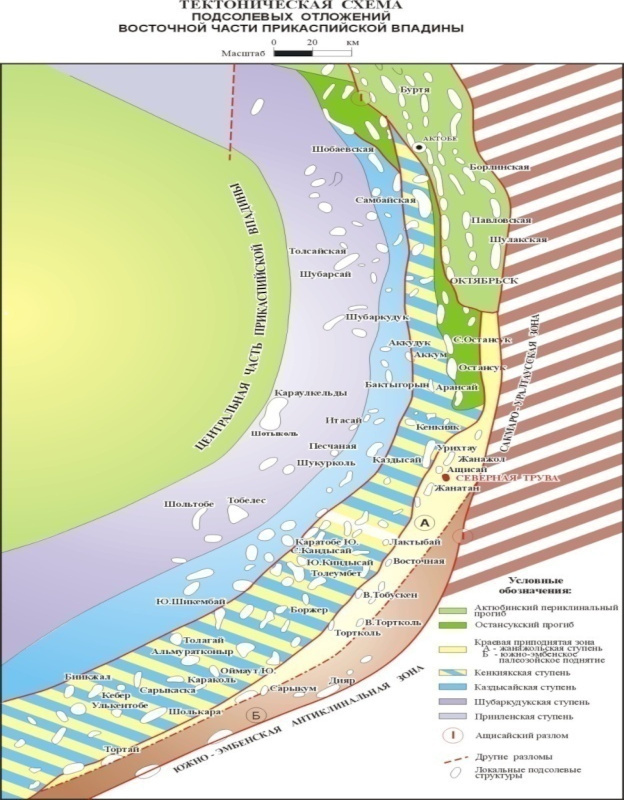
\includegraphics[width=0.8\textwidth]{assets/301}
	\caption*{}
\end{figure}

{\bfseries Рис. 1 - Тектоническая схема подсолевых отложений Восточной
части Прикаспийской впадины}

К основным технологическим факторам, влияющим на показатели нефтедобычи
резервуаров, относятся параметры сети добывающих скважин, основная схема
системы затопления, темпы развития, отбор нагнетательной жидкости,
технология откачки воды и условия развития прилегающих пластов, характер
вскрытия продуктивных пластов в скважинах. Исследование влияние
обводнения продуктивных слоев на полноту добычи, в зависимости от
степени охвата как по площади объекта разработки, так и с точки зрения
рубок, характера перекачиваемой воды и смещения пласта. Поэтому при
геологическом и профессиональном анализе необходимо уделять основное
внимание особенностям движения воды по продуктивным слоям под влиянием
перекачки воды. К числу геологических и физических факторов, влияющих на
процесс слоистого затопления, относятся фильтрующие свойства
продуктивных слоев, их неоднородные свойства и степень их
неоднородности, вязкостные свойства насыщенных слоев и перекачиваемых в
них жидкостей {[}4,5{]}.

Материалы и методы. Нефтяные запасы можно оценить по динамике
интенсивности добычи, коэффициенту текущей подачи нефти и количеству
перекачиваемой воды. Темпы отбора нефти и текущая нефтеотдача
анализируются в динамике по годам развития производства и дате анализа.
Эти показатели определяются для месторождений в целом и для отдельных
районов, блоков, участков и пластов разработки в зависимости от их
первоначальных балансовых запасов {[}6{]}.

Добыча нефтяных запасов также характеризуется темпами добычи нефти из
первичных извлекаемых запасов нефти и текущей передачей нефти.
Балансовые запасы нефти часто используются при попытке избежать ошибок в
определении запасов нефти, а также при сравнительном анализе с другими
месторождениями.

Месторождение Северная Трува в административном отношении расположено на
территории Муголжарского района Актюбинской области Республики
Казахстан.

Нефтегазоносность месторождения связана с отложениями двух карбонатных
толщ. Продуктивные пласты месторождения Северная трува приурочены к
средне-нижнему карбону регионально - нефтегазоносному комплексу пород,
представленному двумя мощными толщами карбонатов (КТ-I и КТ-II),
сложенных из известняка и доломитов {[}7{]}.

В эксплуатационном фонде месторождения Северная Трува добывающих скважин
находятся 164 ед., в том числе 150 действующих, 12 в бездействии, 1 ед.
в освоении и 1 ед. в ожидании освоения после бурения. Скважины
добывающего фонда эксплуатируются механизированным и фонтанным
способами.

С последнего проектного документа «Дополнение к технологической схеме
разработки\ldots» (2015г) на месторождении введены из бурения 38 новых
скважин, из них 3 оценочные скважины, 1 скважина находится в освоении
после бурения, 1 скважина в ожидании освоения:

\begin{itemize}
\item
  Пачка А -- 7 скважин;
\item
  Пачки А+Б -- 3 скважин;
\item
  Пачка Гв-- 10 скважин;
\item
  Пачки Гв+Гн-- 6 скважин;
\item
  Пачка Гн -- 7 скважин.
\end{itemize}

\emph{I объект КТ-1 (А+Б)}

В эксплуатационном фонде добывающих скважин числятся 101ед, а т.ч.
действующие 90, в бездействии 11 скважин. Все скважины кроме скважин
№СТ-24, 484, которые эксплуатируются УЭЦН, работают фонтанным способом
эксплуатации. В освоении после бурения находится одна скважина. 6
скважин эксплуатируются совместно на пачках А+Б.

\emph{II объект -- КТ-2 (Гв+Гн)}

Фонд добывающих скважин составил 63 ед., из них 60 ед. действующие,
скважина №5597 числится в бездействии, скважина №8106 находится в
освоении после бурения и скважина №5633 в ожидании освоения. Также 5
скважин находятся в консервации.

В целом добывающий фонд эксплуатируется фонтанным и механизированным
способами. 59 скважин работают фонтанным способом, 1 скважина (№7615)
газлифтным и 2 скважины (№№7674,7708) НДГ. В целом скважины размещены
равномерно по пачкам.

За отчетный период из бурения в эксплуатацию введено 22 добывающих (1
находится в освоении после бурения, 1 в ожидании освоения после бурения)
и 3 нагнетательных скважин (№№5575, 5617, 5623). Одна добывающая
скважина (СТ-15) была переведена с Iобъекта. 34 добывающих скважин были
переведены в нагнетательный фонд. Стоит заметить, что фонд
нагнетательных скважин увеличился в основном за счёт перевода скважин из
добывающего фонда {[}2,3{]}.

{\bfseries Результаты и обсуждение.} Для оценки эффективности реализуемой
системы разработки месторождения и выработки на этой основе рекомендаций
по совершенствованию системы разработки проведен анализ основных
технологических показателей работы скважин {[}8{]}.

Нефтяная группа определялась на основе трех параметров - воды, хлористых
солей и механических примесей в пробах.

По средним значениям, нефти толщ КТ-I и КТ-II классифицируются как
малосернистые и сернистые и принадлежат первому и второму классам. По
среднему значению нефть толщи KT-I относится к третьей группе: с
содержанием хлористых солей -- 209.2 мг/дм\textsuperscript{3}, - воды --
1.04 мас.\%, - механических примесей не выше нормы. Нефти толщи КТ-II
условно относятся к третьей группе: с содержанием хлористых солей --
641.7 мг/дм\textsuperscript{3}, - воды -- 2.00 мас.\% (выше нормы) -
механических примесей в норме. При этом в общей массе анализов
фиксируются пробы, принадлежащие к первой, второй и третьей группам. По
ряду проб зафиксированы аномальные содержания солей (до 3426
мг/дм\textsuperscript{3}) и воды (8.8 мас.\%), которые не укладываются в
рамки стандарта классификации {[}9{]}.

Потенциал продуктивного горизонта зависит от литологического состава
породы, эффективной мощности~пласта, коллекторских свойств (объёма
порового пространства), степени~нефте-~и (или)~газонасыщения,
величины~вязкости~флюида~и термобарических условий, а также от способов
и интенсивности физико-химических методов воздействия на пласт при
разработке месторождения с целью повышения его~нефте- и
(или)~газоотдачи. Продуктивный горизонт является основным объектом
подсчёта запасов~нефти~и~газа.~На месторождении Северная Трува
пористость вычисляется путем построения кроссплотов по данным
литолого-плотностного каротажа, компенсированного нейтронного каротажа,
акустического каротажа определяется общая пористость, эффективная
пористость выделенных пластов-коллекторов {[}10{]}.

Верхняя карбонатная толща КТ-I, с которой связана
газоконденсатнонефтяная залежь, в стратиграфическом отношении приурочена
к отложениям касимовско-гжельского возраста.

Нижняя карбонатная толща КТ-II, содержащая газонефтеконденсатную залежь,
приурочена к отложениям верейско-каширского возраста. Коллекторские и
физико-химические свойства продуктивных горизонтов указано в таблицах 1
и 2 {[}11{]}.

{\bfseries Таблица 1- Физико-химическая характеристика нефти}

\begin{longtable}[]{@{}
  >{\raggedright\arraybackslash}p{(\columnwidth - 6\tabcolsep) * \real{0.1441}}
  >{\raggedright\arraybackslash}p{(\columnwidth - 6\tabcolsep) * \real{0.3099}}
  >{\raggedright\arraybackslash}p{(\columnwidth - 6\tabcolsep) * \real{0.3246}}
  >{\raggedright\arraybackslash}p{(\columnwidth - 6\tabcolsep) * \real{0.2213}}@{}}
\toprule\noalign{}
\endhead
\bottomrule\noalign{}
\endlastfoot
Объект & Содержание серы & Плотность нефти & Содержание

парафинов \\
КТ-I & до 0,88\% & от 807,0 до 849,0 кг/м\textsuperscript{3} & от 1,67
до 5,20 \% \\
КТ-II & от 0,01 до 1,46\% & от 801,1 до 899,0 кг/м\textsuperscript{3} &
от 1,93 до 4,10 \% \\
\end{longtable}

{\bfseries Таблица 2- Коллекторские свойства продуктивных горизонтов}

\begin{longtable}[]{@{}
  >{\raggedright\arraybackslash}p{(\columnwidth - 10\tabcolsep) * \real{0.1146}}
  >{\raggedright\arraybackslash}p{(\columnwidth - 10\tabcolsep) * \real{0.1919}}
  >{\raggedright\arraybackslash}p{(\columnwidth - 10\tabcolsep) * \real{0.2213}}
  >{\raggedright\arraybackslash}p{(\columnwidth - 10\tabcolsep) * \real{0.1771}}
  >{\raggedright\arraybackslash}p{(\columnwidth - 10\tabcolsep) * \real{0.1181}}
  >{\raggedright\arraybackslash}p{(\columnwidth - 10\tabcolsep) * \real{0.1771}}@{}}
\toprule\noalign{}
\endhead
\bottomrule\noalign{}
\endlastfoot
Объект & Абсолютная глубина & Породы & Общая средняя толщина пласта &
Порис-

тость & Проницае-мость \\
КТ-I & 2095 -- 2510м & известняки, доломиты, с прослойками терригенных,
преимущественно аргиллитовых пород & 466м & 15,19\% & 34,02 мД \\
КТ-II & 2843 -- 3021м & известняки с прослоями зеленовато-серых
аргиллитов и доломитов & 320м & 12\% & 56,6 мД \\
\end{longtable}

Анализ текущих среднесуточных показателей работы скважин и динамика
распределения действующего фонда по дебитам нефти показана в таблице 3.
Согласно проведенному распределению фонда добывающих скважин по дебитам
нефти большая часть скважин работает с дебитами до 5 т/сут -- 40,7\% от
действующего фонда скважин месторождения и большинство из них
эксплуатируются на I объекте, доля которых там составляет 57,2\%, тогда
как их доля на IIобъекте не превышает 15\%. Однако стоит учитывать, что
значительная часть из данных скважин работают периодически. Скважины со
средним дебитом от 10 до 25т/сут занимают 26\% всего действующего фонда.
Также к скважинам со сравнительно высоким дебитом от 25 т/сут относится
20,7\% действующего фонда, большинство из которых эксплуатируются на
IIобъекте. Остальные 12\% скважин на месторождении эксплуатируются с
дебитом от 5 до 10т/сут. Из данного распределения скважин по дебитам,
можно сделать вывод, что скважины IIобъекта характеризуются более
высокими дебитами по сравнению с I объектом {[}2,3{]}.

Таблица 3- Динамика распределения действующего фонда по дебитам нефти по
объектам на 01.01.2022 г

\begin{longtable}[]{@{}
  >{\raggedright\arraybackslash}p{(\columnwidth - 10\tabcolsep) * \real{0.1706}}
  >{\raggedright\arraybackslash}p{(\columnwidth - 10\tabcolsep) * \real{0.1718}}
  >{\raggedright\arraybackslash}p{(\columnwidth - 10\tabcolsep) * \real{0.1404}}
  >{\raggedright\arraybackslash}p{(\columnwidth - 10\tabcolsep) * \real{0.1560}}
  >{\raggedright\arraybackslash}p{(\columnwidth - 10\tabcolsep) * \real{0.1557}}
  >{\raggedright\arraybackslash}p{(\columnwidth - 10\tabcolsep) * \real{0.2055}}@{}}
\toprule\noalign{}
\multicolumn{3}{@{}>{\raggedright\arraybackslash}p{(\columnwidth - 10\tabcolsep) * \real{0.4828} + 4\tabcolsep}}{%
\begin{minipage}[b]{\linewidth}\raggedright
Объект
\end{minipage}} & \begin{minipage}[b]{\linewidth}\raggedright
КТ-1
\end{minipage} & \begin{minipage}[b]{\linewidth}\raggedright
КТ-2
\end{minipage} & \begin{minipage}[b]{\linewidth}\raggedright
Месторождение
\end{minipage} \\
\midrule\noalign{}
\endhead
\bottomrule\noalign{}
\endlastfoot
\multicolumn{3}{@{}>{\raggedright\arraybackslash}p{(\columnwidth - 10\tabcolsep) * \real{0.4828} + 4\tabcolsep}}{%
Фонд скважин} & 90 & 60 & 150 \\
\multicolumn{3}{@{}>{\raggedright\arraybackslash}p{(\columnwidth - 10\tabcolsep) * \real{0.4828} + 4\tabcolsep}}{%
Средний дебит нефти} & 8,6 & 20,9 & 13,5 \\
\multirow{10}{=}{Диапазон изменения дебитов нефти, т/сут} &
\multirow{2}{=}{q≤5} & Кол-во & 52 & 9 & 61 \\
& & \% & 57,8 & 15,0 & 40,7 \\
& \multirow{2}{=}{5\textless q≤10} & Кол-во & 12 & 6 & 18 \\
& & \% & 13,3 & 10,0 & 12,0 \\
& \multirow{2}{=}{10\textless q≤25} & Кол-во & 17 & 23 & 40 \\
& & \% & 18,9 & 38,3 & 26,7 \\
& \multirow{2}{=}{25\textless q≤50} & Кол-во & 8 & 17 & 25 \\
& & \% & 8,9 & 28,3 & 16,7 \\
& \multirow{2}{=}{50≥q} & Кол-во & 1 & 5 & 6 \\
& & \% & 1,1 & 8,3 & 4,0 \\
\end{longtable}

Интенсификация отборов нефти на месторождении сопровождается высокими
показателями газового фактора по I и II объекту, который на дату отчета
по составил 964 и 985 м\textsuperscript{3}/т объектам соответственно.

Как видно из таблицы 4 по распределению газового фактора видно, что
наибольшая часть скважин по объектам и соответственно по всему
месторождению (84\%) работают с показателями по газовому фактору от 900
до 1000 м\textsuperscript{3}/т. Со значениями газового фактора менее
900м\textsuperscript{3}/т и в диапазоне от 1000 до 1100
м\textsuperscript{3}/т эксплуатируются оставшиеся 16 \% действующего
фонда добывающих скважин месторождения.

Высокий газовый фактор по некоторым скважинам обусловлен возможным
дегазацией скважин, ак как наблюдается падения пластового давления ниже
давления насыщения. По данному фонду рекомендуется перевести скважины в
бездействия или перевести на более щадящий режим разработки, с
проведением периодических ГДИС, с целью прослеживания динамики
восстановления пластового давления. Прорыв из газовой шапки возможен,
однако перфорация скважин не охватывает интервалы насыщенности газа,
рекомендуется провести ГИС исследования по определению текущего
положения насыщения.

{\bfseries Таблица 4- Динамика распределения фонда скважин по газовому
фактору}

\begin{longtable}[]{@{}
  >{\raggedright\arraybackslash}p{(\columnwidth - 10\tabcolsep) * \real{0.1628}}
  >{\raggedright\arraybackslash}p{(\columnwidth - 10\tabcolsep) * \real{0.1917}}
  >{\raggedright\arraybackslash}p{(\columnwidth - 10\tabcolsep) * \real{0.1361}}
  >{\raggedright\arraybackslash}p{(\columnwidth - 10\tabcolsep) * \real{0.1531}}
  >{\raggedright\arraybackslash}p{(\columnwidth - 10\tabcolsep) * \real{0.1511}}
  >{\raggedright\arraybackslash}p{(\columnwidth - 10\tabcolsep) * \real{0.2052}}@{}}
\toprule\noalign{}
\multicolumn{3}{@{}>{\raggedright\arraybackslash}p{(\columnwidth - 10\tabcolsep) * \real{0.4906} + 4\tabcolsep}}{%
\begin{minipage}[b]{\linewidth}\raggedright
Объект
\end{minipage}} & \begin{minipage}[b]{\linewidth}\raggedright
КТ-1
\end{minipage} & \begin{minipage}[b]{\linewidth}\raggedright
КТ-2
\end{minipage} & \begin{minipage}[b]{\linewidth}\raggedright
Месторождение
\end{minipage} \\
\midrule\noalign{}
\endhead
\bottomrule\noalign{}
\endlastfoot
\multicolumn{3}{@{}>{\raggedright\arraybackslash}p{(\columnwidth - 10\tabcolsep) * \real{0.4906} + 4\tabcolsep}}{%
Фонд скважин} & 90 & 60 & 150 \\
\multicolumn{3}{@{}>{\raggedright\arraybackslash}p{(\columnwidth - 10\tabcolsep) * \real{0.4906} + 4\tabcolsep}}{%
Средний газовый фактор} & 964,4 & 984,9 & 972,6 \\
\multirow{10}{=}{Диапазон изменения газового фактора,
м\textsuperscript{3}/т} & \multirow{2}{=}{ГФ≤800} & Кол-во & 3 & 1 &
4 \\
& & \% & 3,3 & 1,7 & 2,7 \\
& \multirow{2}{=}{800\textless ГФ≤900} & Кол-во & 11 & 1 & 12 \\
& & \% & 12,2 & 1,7 & 8,0 \\
& \multirow{2}{=}{900\textless ГФ≤1000} & Кол-во & 71 & 55 & 126 \\
& & \% & 78,9 & 91,7 & 84,0 \\
& \multirow{2}{=}{1000\textless ГФ≤1100} & Кол-во & 5 & 3 & 8 \\
& & \% & 5,6 & 5,0 & 5,3 \\
& \multirow{2}{=}{1100\textless ГФ} & Кол-во & 0 & 0 & 0 \\
& & \% & 0,0 & 0,0 & 0,0 \\
\end{longtable}

В целом по месторождению высокий коэффициент эксплуатации и в среднем
составил 0,98 доли единиц: по Iобъекту 0,98 доли ед. и по II объекту
0,97доли единиц.

Касательно коэффициента использования фонда. Данный показатель по
месторождению составляет 0,91. Основная доли низкого коэффициента
использования сосредоточена на I объекте разработки, где находится
основной фонд бездействующих скважин по причине проведения ГТМ. По II
объекту коэффициент использования фонда ближе единице и составляет 0,95
доли единиц. По данному объекту всего одна скважина находится в
бездействии {[}3,5{]}.

Анализ эксплуатации скважин, устьевого и внутрискважинного оборудования

Для герметизации устья скважин и разобщения межтрубного пространства
между НКТ и эксплуатационной колонны, направления продукции скважины в
систему сбора, а также регулирования режима работы скважины на устье
скважин установлены фонтанные арматуры \emph{KYS35/80-65-1 (КНР)},
рассчитанные на рабочее давление 35 МПа, с условным проходом стволовой
части ёлки 80 мм и боковых отводов 65 мм. В фонтанную арматуру входят
колонная головка, трубная головка и фонтанная ёлка {[}12,13{]}.

Арматура изготовлена в антикоррозионном исполнении для среды, содержащей
Н\textsubscript{2}S и СО\textsubscript{2}.

Изменение режима работы скважины осуществляется с помощью штуцеров,
установленных на боковых отводах фонтанной елки, на I объекте штуцеры
изменяются от 3 до 20мм, на II объекте от 3 до 25мм.

Фонтанная елка имеет по два запорных устройства на каждый отвод (один
рабочий, другой запасной) которые рассчитаны на рабочее давление 35 МПа.
Диаметр боковых отводов может быть увеличен с учетом применения в
системе сбора шлейфа большего диаметра. Боковые выкиды арматуры
оборудованы штуцеродержателями для установки щтуцеров и фонтанными
клапанами или дроссельными устройствами.

Внутрискважинное оборудование

Подземное оборудование (ПО) скважин позволяет осуществлять эксплуатацию
скважины на установленном технологическом режиме, освоение, исследование
и остановку скважины без задавки её жидкостью, воздействие на
призабойную зону пласта с целью интенсификации притока к скважине, а
также защиту скважины от открытого фонтанирования.

Внутрискважинное оборудование фонтанных скважин состоит из
двухступенчатого подъемника, составленного из насосно-компрессорных труб
(НКТ) с наружными диаметрами 73 мм и 88,9 мм, что является рациональным
в условиях эксплуатации месторождения. НКТ Ø89,9 имеет толщину 6,45мм,
Ø73 мм- 7,01 мм.

Для надёжной эксплуатации скважин нефтегазоконденсатного месторождения
исходя из условий эксплуатации, используется следующее подземное
оборудование:

\begin{itemize}
\item
  насосно-компрессорные трубы;
\item
  разобщитель (пакер);
\item
  клапан-отсекатель для автоматического закрытия центрального канала
  скважины;
\item
  башмак колонны НКТ оборудован воронкой в нижней части, которые спущены
  в эксплуатационную колонну диаметром 168,3 и 177,8 мм.
\end{itemize}

Фонтанная арматура скважин соединяется с промысловыми коммуникациями
сбора пластовой жидкости с помощью манифольда, служащего для подключения
к трубному и затрубному пространствам агрегатов для проведения различных
операций при пуске и эксплуатации скважины.

Выбор НКТ Ø89 и Ø73 мм основан на удовлетворении требованиям при КГРП.

В нефтяной залежи KT-I используется комбинированная колонна( Ø89 и Ø73
мм), в которой НКТ Ø89 мм (толщина 6,45 мм) будет иметь длину до 500 м.
В нефтяной залежи KT-IIтакже используется комбинированная колонна, в
которой НКТ Ø89 мм (толщина 6,45 мм), будет длиной 500 м-1000м.

Для обеспечения поддержания высокого устьевого давления при фонтанной
эксплуатации необходим правильный выбор диаметра НКТ. Проведенные
расчеты (Рисунок 2 и 3) определяют использование на месторождении
Северная Трува комбинированных НКТ Ø88,9 мм (толщина 6,45мм) и Ø73 мм
(толщина 7,01мм) {[}14{]}.

\begin{figure}[H]
	\centering
	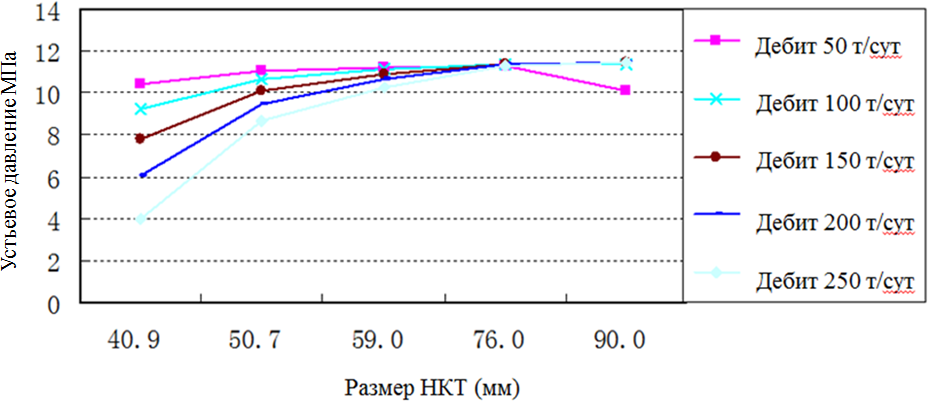
\includegraphics[width=0.8\textwidth]{assets/302}
	\caption*{}
\end{figure}

{\bfseries Рис. 2 - Зависимость устьевого давления от диаметра НКТ (KT-I)}

\begin{figure}[H]
	\centering
	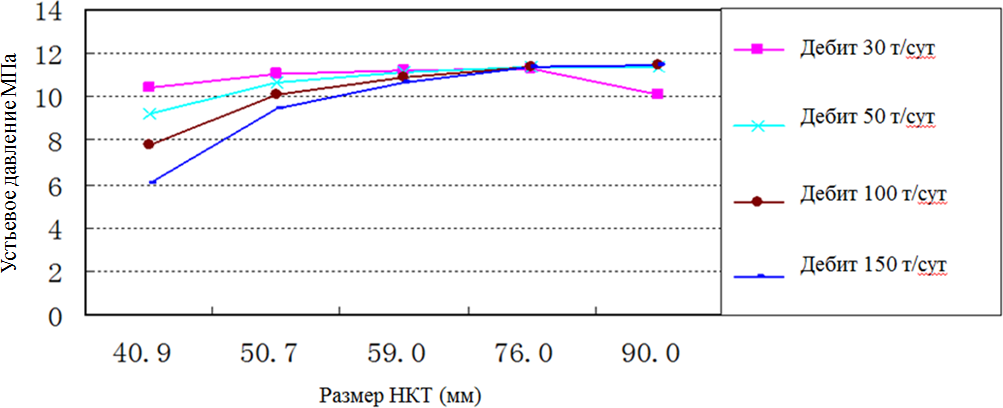
\includegraphics[width=0.8\textwidth]{assets/303}
	\caption*{}
\end{figure}

{\bfseries Рис. 3 - Зависимость устьевого давления от диаметра НКТ (KT-II)}

Выводы. На основании расчетов, были определены минимальные давления,
обводненность и другие факторы, при которых скважины прекращают
фонтанирование, что позволяет прогнозировать количество скважин и время
перевода скважин на механизированный способ добычи.

Минимальное устьевое давление прекращения фонтанирования составляет 2
МПа, при этом среднее пластовое давление по I объекту составляет 21 МПа,
среднесуточный дебит скважин -- 100 м\textsuperscript{3}/сут,
обводненность -- 2,8\%, газовый фактор -- 242,8
м\textsuperscript{3}/м\textsuperscript{3}. Согласно проведенным расчетам
в 2021г пластовое давление снизится до 18,8 МПа. Затем панируется рост
пластового давления до 20 МПа, обусловленное влиянием реализации
полномасштабной системы ППД закачкой воды.

По мере повышения объема закачиваемой воды обводненность постепенно
увеличивается, и в 2030г обводненность достигнет 81,2 \%. По прогнозу в
2012г в толще KT-I начнется прекращение фонтанирования, 2023 - 2030гг
являются пиком прекращения фонтанирования, после 2030г основная доля
фонда скважин переводится на механизированный способ эксплуатации.

Среднее пластовое давление по II объекту составляет 29,4 МПа,
среднесуточный дебит скважин -- 48 м\textsuperscript{3}/сут,
обводненность -- 3,9 \%, газовый фактор -- 454
м\textsuperscript{3}/м\textsuperscript{3}. До 2022г согласно выполненным
расчетам пластовое давление будет снижаться до 26,6 МПа, в 2022г, за
счет полномасштабного внедрения системы ППД, наблюдается стабилизация
снижение пластового давления до 2029 года, далее наблюдается тенденция
снижения.

По мере повышения объема закачиваемой воды обводненность продукции
постепенно увеличивается, и в 2030г обводненность продукции достигнет
88,9\%. По прогнозу в 2012г в толще KT-II начнется прекращение
фонтанирования скважин, 2019-2030гг являются пиком прекращения
фонтанирования скважин, после 2030г основная доля фонда скважин
переводится на механизированный способ эксплуатации.

{\bfseries Литература}

\begin{enumerate}
\def\labelenumi{\arabic{enumi}.}
\item
  В.Н. Бабашев, А.К. Габбасова и др. «Дополнение №1 к проекту оценочных
  работ на месторождении Северная Трува»: Отчет, - Алматы: 2015.
\end{enumerate}

URL: file:///C:/Users/User/Downloads/PDF\%20(2).pdf

\begin{enumerate}
\def\labelenumi{\arabic{enumi}.}
\setcounter{enumi}{1}
\item
  Отчет «СНПС Актобемунайгаз», 2023. URL:
  http://www.cnpc-amg.kz/?p=senm\_11
\item
  Групповой технический проект на строительство скважин № 7764, 7804,
  829, 538, Н828, 595 месторождения Северная Трува. -Актобе, 2021. URL:
\end{enumerate}

https://www.gov.kz/uploads/2021/12/22/1f923b8735e172674f2771b9b2b72159\_original.1330537.pdf

\begin{enumerate}
\def\labelenumi{\arabic{enumi}.}
\setcounter{enumi}{3}
\item
  Джиембаева, К.И., Ахмеджанов Т.К., М. К. Сакиев М.К. Техника и
  технология добычи нефти: учебное пособие, - Алматы: Экономика, 2011.
  -300 с. ISBN~978-601-225-279-8.
\item
  Арбузов В.Н. Эксплуатация нефтяных и газовых скважин. Часть 1: учебное
  пособие. -- Томск: ТПУ, 2011. -200 с.
\item
  Покрепин Б.В., Гумаров Г.С, Нугманов М.А. Добыча нефти и газа: учебное
  пособие. -- Астана: Фолиант, 2011.-392 с. (Профессиональное
  образование) ISBN 978-601-292-338-4~
\item
  Мищенко И.Т. Скважинная добыча нефти - Москва: Издательский центр РГУ
  нефти и газа им. И.М. Губкина, 2015. - 448 с. ISBN 978-5-91961-145-5
\item
  Лалазарян Н.В. Эксплуатация нефтяных и газовых скважин. Учебное
  пособие. - Алматы: КазНТУ, 2008 -- 140 с. ISBN 978-601-228-026-5
\item
  Воцалевский Э.С.,~Даукеев С.Ж.,~Коломиец В.П.,~Комаров
  В.П.,~Парагульгов Х.Х.,~Пилифосов В.М.,~Шлыгин Д.А., С.Ж. Даукеев.
  Глубинное строение и минеральные ресурсы Казахстана //Нефть и газ.
  -Алматы, 2002.- Т. III. -248 с. ISBN 9965-13-760-9.
\item
  М.Н. Персиянцев. Добыча нефти в осложненных условиях. -М.:Недра, 2000.
  -653 с. ISBN 5-8365-0052-5.
\item
  Газизов А.А. Увеличение нефтеотдачи неоднородных пластов на поздней
  стадии разпаботки. --М.: ООО Недра-бизнесцентр, 2002. -639 с. ISBN
  5-8365-0119-X.
\item
  Методические указания по геолого-промысловому анализу разработки
  нефтяных и газонефтяных месторождений (РД 153-39.0-110-01).
  -Типография "Наука", 121099, Москва,2001.
  https://files.stroyinf.ru/Data2/1/4293816/4293816261.pdf
\item
  Федорова К.В., Кривова Н.Р, Колесник С.В., Решетникова Д.С. Анализ
  состояния выработки запасов нефти из пластов покурской свиты //
  Геология, геофизика и разработка нефтяных и газовых месторождений.-
  2014. - № 11.- С. 54-58. ISSN 0234-1581
\item
  Аржиловский А.В., Гусева Д.Н. Сравнение методов анализ выработки
  остаточных запасов // Нефтепромысловое дело. -2016. -№ 10. - С. 14-19.
  ~ISSN 0207-2351.
\end{enumerate}

References

1. V.N. Babashev, A.K. Gabbasova i dr. «Dopolnenie №1 k proektu
ocenochnyh rabot na mestorozhdenii Severnaja Truva»: Otchet, - Almaty:
2015.

URL: file:///C:/Users/User/Downloads/PDF\%20(2).pdf {[}in Russian{]}

2. Otchet «SNPS Aktobemunajgaz», 2023. URL:
http://www.cnpc-amg.kz/?p=senm\_11 {[}in Russian{]}

3. Gruppovoj tehnicheskij proekt na stroitel\textquotesingle stvo
skvazhin № 7764, 7804, 829, 538, N828, 595 mestorozhdenija Severnaja
Truva. -Aktobe, 2021. URL:

https://www.gov.kz/uploads/2021/12/22/1f923b8735e172674f2771b9b2b72159\_original.1330537.pdf
{[}in Russian{]}

4. Dzhiembaeva, K.I., Ahmedzhanov T.K., M. K. Sakiev M.K. Tehnika i
tehnologija dobychi nefti: uchebnoe posobie, - Almaty: Jekonomika, 2011.
-300 s. ISBN 978-601-225-279-8. {[}in Russian{]}

5. Arbuzov V.N. Jekspluatacija neftjanyh i gazovyh skvazhin.
Chast\textquotesingle{} 1: uchebnoe posobie. -- Tomsk: TPU, 2011. -200
s. {[}in Russian{]}

6. Pokrepin B.V., Gumarov G.S, Nugmanov M.A. Dobycha nefti i gaza:
uchebnoe posobie. -- Astana: Foliant, 2011.-392 s.
(Professional\textquotesingle noe obrazovanie) ISBN 978-601-292-338-4.
{[}in Russian{]}

7. Mishhenko I.T. Skvazhinnaja dobycha nefti - Moskva:
Izdatel\textquotesingle skij centr RGU nefti i gaza im. I.M. Gubkina,
2015. -448 s. ISBN 978-5-91961-145-5. {[}in Russian{]}

8. Lalazarjan N.V. Jekspluatacija neftjanyh i gazovyh skvazhin. Uchebnoe
posobie. - Almaty: KazNTU, 2008 - 140 s. ISBN 978-601-228-026-5. {[}in
Russian{]}

9. Vocalevskij Je.S., Daukeev S.Zh., Kolomiec V.P., Komarov V.P.,
Paragul\textquotesingle gov H.H., Pilifosov V.M., Shlygin D.A., S.Zh.
Daukeev. Glubinnoe stroenie i mineral\textquotesingle nye resursy
Kazahstana //Neft\textquotesingle{} i gaz. -Almaty, 2002.- T. III. -248
s. ISBN: 9965-13-760-9. {[}in Russian{]}

10. M.N. Persijancev. Dobycha nefti v oslozhnennyh uslovijah. -M.:Nedra,
2000. -653 s. ISBN: 5-8365-0052-5. {[}in Russian{]}

11. Gazizov A.A. Uvelichenie nefteotdachi neodnorodnyh plastov na
pozdnej stadii razpabotki. --M.: OOO Nedra-biznescentr, 2002. -639 s.
ISBN 5-8365-0119-X. {[}in Russian{]}

12. Metodicheskie ukazanija po geologo-promyslovomu analizu razrabotki
neftjanyh i gazoneftjanyh mestorozhdenij (RD 153-39.0-110-01).
-Tipografija "Nauka", 121099, Moskva,2001.
https://files.stroyinf.ru/Data2/1/4293816/4293816261.pdf {[}in
Russian{]}

13. Fedorova K.V., Krivova N.R, Kolesnik S.V., Reshetnikova D.S. Analiz
sostojanija vyrabotki zapasov nefti iz plastov pokurskoj svity //
Geologija, geofizika i razrabotka neftjanyh i gazovyh mestorozhdenij.
-2014.- № 11.- S. 54-58. ISSN 0234-1581 {[}in Russian{]}

14. Arzhilovskij A.V., Guseva D.N. Sravnenie metodov analiz vyrabotki
ostatochnyh zapasov // Neftepromyslovoe delo. -2016. -№ 10. - S. 14-19.
ISSN 0207-2351. {[}in Russian{]}

Сведения об авторах

Кайненова Т.С. - магистр, старший преподаватель, Актюбинский
региональный университет им. К.Жубанова, Актобе, Казахстан, е-mail:
kaynenova83@mail.ru;

Космбаева Г.Т. - cтарший преподаватель кафедры «Нефтегазовое дело»
Актюбинского регионального университета им. К. Жубанова, Актобе,
Казахстан, е-mail: gulzhank\_67@mail.ru;

Отарбаева А.Т. - магистр, преподаватель кафедры «Нефтегазовое дело»,
Актюбинский региональный университет им. К. Жубанова, Актобе, Казахстан,
е-mail: ainaerlan1984@mail.ru;

Мерекеқызы А. - cтарший преподаватель кафедры «Нефтегазовое дело»
Актюбинского регионального университета им. К. Жубанова, Актобе,
Казахстан, е-mail: ardak.merekekyzy@mail.ru.

Information about the authors

Kainenova T.S. - Master of Technical Sciences, senior Lecturer, Aktobe
Regional University named after K. Zhubanov, Kazakhstan. е-mail:
kaynenova83@mail.ru;

Kosmbayeva G.T. - Senior Lecturer, Aktobe Regional University named
after K. Zhubanov, Kazakhstan. е-mail: gulzhank\_67@mail.ru;

Otarbayeva A.T. - Master of Technical Sciences, Lecturer, Aktobe
Regional University named after K. Zhubanov, Kazakhstan. е-mail:
ainaerlan1984@mail.ru{\bfseries ;}

Merekeqyzy A. - Senior Lecturer, Aktobe Regional University named after
K. Zhubanov, Kazakhstan. е-mail: ardak.merekekyzy@mail.ru.\newpage
{\bfseries IRSTI 55.39.01}

{\bfseries ENSURING RELIABLE AND SAFE OIL STORAGE IN THE}

{\bfseries REPUBLIC OF KAZAKHSTAN}

{\bfseries \textsuperscript{1}N.T. Smailova\textsuperscript{🖂}, A.Y.
Popov\textsuperscript{2}}

\textsuperscript{1} Kazakh University of Technology and Business named
after K.Kulazhanov, Astana, Kazakhstan

\textsuperscript{2} Omsk State Technical University, Omsk, Russian
Federation

{\bfseries \textsuperscript{🖂}}Correspondent-author: ganibek2006@mail.ru

The article highlights the issue of possible construction of the first
large oil storage facility in the history of Kazakhstan. Construction of
large oil storage facilities in Kazakhstan is an important step to
ensure efficient storage and management of oil products in the country,
solving the problem of redistribution and storage of oil products, given
the dynamics of production and consumption growth in the country.
Construction of a large oil storage facility in Atyrau region, as well
as oil depots in the west of Kazakhstan, will optimize the processes of
transportation and storage of oil products, reduce the cost of renting
other people\textquotesingle s storage facilities and ensure the
sustainability and reliability of oil products supplies to both domestic
and foreign markets. The article considers such important aspects as the
need for storage of oil products, technical and environmental aspects of
construction, as well as economic and social feasibility. In addition,
the article presents a system analysis and study of the potential for
construction of a large oil storage facility in Kazakhstan, which makes
it significant and relevant in the context of the development of the
country\textquotesingle s oil and gas industry. Given the current global
challenges, such as oil production limitations and volatility of oil and
oil products markets, the strategic reserve becomes even more relevant.

{\bfseries Key words:} hydrocarbon feedstock, storage of petroleum
products, strategic reserve, provision of domestic needs.

{\bfseries ҚАЗАҚСТАН РЕСПУБЛИКАСЫНДА МҰНАЙДЫҢ СЕНІМДІ}

{\bfseries ЖӘНЕ ҚАУІПСІЗ САҚТАЛУЫН ҚАМТАМАСЫЗ ЕТУ}

{\bfseries \textsuperscript{1}Н.Т. Смайлова\textsuperscript{🖂},
\textsuperscript{2}А.Ю. Попов}

\textsuperscript{1} Қ. Құлажанов атыңдағы Қазақ технология және бизнес
университеті, Астана, Қазақстан,

\textsuperscript{2}Омбы мемлекеттік техникалық университеті, Омбы,
Ресей,

email: ganibek2006@mail.ru

Мақалада Қазақстан тарихындағы алғашқы ірі мұнай қоймасын салу
мүмкіндігі туралы мәселе көтерілген. Қазақстанда ірі мұнай қоймаларының
құрылысы республикада мұнай өнімдерін тиімді сақтау мен басқаруды
қамтамасыз ету, мұнай өнімдерін қайта бөлу және сақтау мәселесін шешу,
мұнай өнімдерін өндіру мен тұтынудың өсу динамикасын ескере отырып,
маңызды қадам болып табылады. Атырау облысында ірі мұнай сақтау
қоймасының, сондай-ақ Қазақстанның батысындағы мұнай базаларының
құрылысы мұнай өнімдерін тасымалдау және сақтау процестерін
оңтайландыруға, шетелдік қоймаларды жалға алу құнын төмендетуге және
жеткізілімдердің тұрақтылығы мен сенімділігін қамтамасыз етуге мүмкіндік
береді және мұнай өнімдерін ішкі және сыртқы нарыққа шығару. Мақалада
мұнай өнімдерін сақтау қажеттілігі, құрылыстың техникалық және
экологиялық аспектілері, сондай-ақ экономикалық және әлеуметтік
орындылығы сияқты маңызды аспектілер қарастырылады. Сонымен қатар,
мақалада Қазақстандағы ірі мұнай қоймасын салу әлеуетін жүйелі талдау
және зерделеу ұсынылған, бұл оны еліміздің мұнай-газ саласын дамыту
контекстінде маңызды және өзекті етеді. Мұнай өндіруді шектеу және мұнай
мен мұнай өнімдері нарығындағы құбылмалылық сияқты ағымдағы жаһандық
сын-қатерлерді ескере отырып, стратегиялық резерв бұрынғыдан да өзекті
бола түседі.

{\bfseries Түйін сөздер:} көмірсутегі шикізаты, мұнай өнімдерін сақтау,
стратегиялық резерв, ішкі қажеттіліктерді қамтамасыз ету.

{\bfseries ОБЕСПЕЧЕНИЕ НАДЕЖНОГО И БЕЗОПАСНОГО ХРАНЕНИЯ НЕФТИ}

{\bfseries В РЕСПУБЛИКЕ КАЗАХСТАН}

{\bfseries \textsuperscript{1}Н.Т.Смайлова\textsuperscript{🖂},
\textsuperscript{2}А.Ю.Попов}

\textsuperscript{1}Казахский университет технологии и бизнеса им. К.
Кулажанова,

г. Астана, Казахстан,

\textsuperscript{2}Омский государственный технический университет,
г.Омск, Россия,

email: ganibek2006@mail.ru .

В статье освещается вопрос возможного строительства первого в истории
Казахстана крупного нефтехранилища. Строительство крупных нефтехранилищ
в Казахстане представляет собой важный шаг для обеспечения эффективного
хранения и управления нефтепродуктами в стране, решение проблемы
перераспределения и хранения нефтепродуктов, учитывая динамику роста
производства и потребления в стране. Строительство крупного
нефтехранилища в Атырауской области, а также нефтебаз на западе
Казахстана, позволит оптимизировать процессы транспортировки и хранения
нефтепродуктов, снизить затраты на аренду чужих хранилищ и обеспечить
устойчивость и надежность поставок нефтепродуктов как на внутренний, так
и на внешний рынки. В статье рассматриваются такие важные аспекты, как
потребность в хранении нефтепродуктов, технические и экологические
аспекты строительства, а также экономическая и социальная
целесообразность. Кроме того, в статье представлен системный анализ и
исследование потенциала строительства крупного нефтехранилища в
Казахстане, что делает ее значимой и актуальной в контексте развития
нефтегазовой отрасли страны. Учитывая текущие глобальные вызовы, такие
как ограничения добычи нефти и волатильность рынков нефти и
нефтепродуктов, стратегический резерв становится еще более актуальным.

{\bfseries Ключевые слова:} углеводородное сырье, хранение нефтепродуктов,
стратегический резерв, обеспечение внутренних потребностей.

{\bfseries Introduction.} Kasym-Jomart Tokayev called one of the most
urgent tasks to increase the capacity of oil storage facilities, as
producers are forced to immediately send raw materials for export, as it
is required by technology. In this regard, the President instructed to
consider the construction of a large oil storage facility taking into
account environmental requirements. {[}1{]}

The oil and gas sector deals with all aspects of the extraction,
production, transportation and use of oil. This sector plays a key role
in the world economy as oil is a potential source of energy used in
various industries. {[}2{]}

Kazakhstan exports oil in unrefined form and then imports petroleum
products, this results in loss of value added and reduced economic
efficiency.

To address this problem, a number of factors need to be considered:

- Production structure:

Determining the optimal oil transportation and refining scheme depends
on the specifics of the fields and infrastructure in the production
regions. Some fields may be more favorable for direct on-site refining
and storage, while for others it may make more sense to export crude
oil.

- Technological Capabilities:

Assess technological opportunities for domestic crude oil storage and
refining. The feasibility of oil storage facilities, the capacity of
refineries, and the potential for modernization and expansion of these
refineries should be explored.

- Economic aspects:

Conduct a cost-benefit analysis of the construction of oil storage
facilities and various oil transportation and refining schemes. This
includes the cost of investment in the construction of oil storage
facilities, refinery upgrades, and the cost of transporting petroleum
products.

\emph{Feasibility of large underground storage facilities.}
Kazakhstan\textquotesingle s President Kassym-Jomart
Tokayev\textquotesingle s raising of the issue of large oil storage
facilities indicates the importance of providing the country with a
reliable infrastructure for storage and management of oil products,
strengthening the security of oil supplies, ensuring stability in the
domestic market and increasing independence from external factors such
as transportation constraints or geopolitical tensions.

The construction of oil storage facilities will ensure the development
of infrastructure and economic potential of the region, as the
construction of oil storage facilities can create jobs and contribute to
the development of the local economy.

Underground oil storage facilities allow for the creation of significant
reserves of crude oil and petroleum products in a small footprint.
Compared to above-ground oil storage facilities, they are safer,
characterized by lower evaporation losses, lower heat consumption to
maintain the required temperature in the storage facility and lower
specific costs of construction and operation. Underground oil storage
facilities include underground tanks (tank workings, auxiliary mine
workings, wells, etc.), surface buildings and structures. Due to floods
that began in March 2024, oil wells in western Kazakhstan were flooded,
especially in the Atyrau region, where most of the
country\textquotesingle s oil reserves are located. Three of the flooded
wells are located in the East Uaz field - \#101, \#106, \#116 (JSC
Embamunaigas oil and gas production department Kainarmunaigas). Another
well is located at Zhana Makat field - No. E7 (5A Oil LLP). Faced with
such a problem, having an underground oil storage facility is one of the
strategies to minimize the risks associated with floods and other
natural disasters. Unlike above-ground oil storage facilities,
underground storage facilities can be more protected from natural
disasters: floods, earthquakes or fires.

This is a serious problem for oil producers in Aktobe and Atyrau regions
due to the flood situation. The suspension of 634 wells and the loss of
16 thousand tons of oil has a significant impact on production and on
the economy of the country as a whole. It will also lead to negative
consequences for the environment and the health of the local population.

Large underground storage facilities play an important role in ensuring
the reliability and sustainability of the upstream and downstream
industry, as well as protecting strategic reserves. Here are some of the
tasks they accomplish:

- Stockpiling reserves to cover peak fluctuations, underground storage
facilities allow oil and petroleum products to be stockpiled during
periods of low demand or excess production to provide coverage for peak
demand fluctuations or supply problems.

- Protecting strategic reserves, large underground storage facilities
provide a safe and secure place to store strategically important
hydrocarbon reserves to ensure preparedness to deal with emergencies or
crises.

- Ensuring uninterrupted operations of production, refining and
transportation facilities, underground storage facilities help to ensure
a stable supply of oil and petroleum products to production, refining
and transportation facilities, preventing downtime and reducing the risk
of interruption to operations.

- Ensuring the reliability of the storage system, large underground
storage facilities have high capacity and reliability, making them an
important link in the hydrocarbon storage system, helping to ensure the
stability of the industry and the sustainability of the
country\textquotesingle s energy system.

\begin{figure}[H]
	\centering
	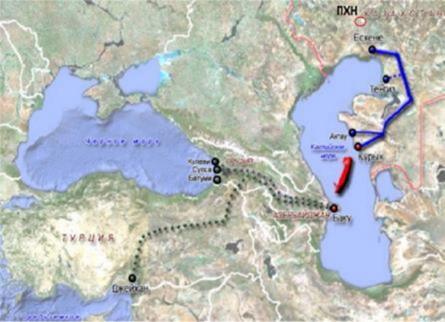
\includegraphics[width=0.8\textwidth]{assets/304}
	\caption*{}
\end{figure}

{\bfseries Figure 1 - Location of the planned underground oil storage
facility located in Inder district}

{\bfseries of Atyrau region}

{\bfseries Materials and methods.} The underground oil storage project will
help stabilize Kazakhstan\textquotesingle s oil production,
transportation and storage. The discovery of an old abandoned
underground salt mine, presents significant prospects and a number of
advantages of using the space of this mine for the construction of
underground oil storage. {[}3{]}

It is proposed to create with relatively low investment underground
storage in salt deposits, in the depleted salt mines of Inder. Inder is
located in Atyrau region, and on the way of main oil pipelines
Karachaganak-KTK, Atyrau-Samara. The technology of CCS has been tested
worldwide, i.e. storage in salt domes is cheaper, safer, less negative
impact on the environment, and there are practically no operating costs
compared to ground equipment.

The cost of storage is several times cheaper than above-ground storage
tanks. And due to the fact that oil will be stored at a depth of 300
meters (in the Caspian region 200 meters below sea level), it will
preserve the temperature regime and pressure for oil, and as a
consequence of preserving the quality of oil for a long time. {[}4{]}

Geographical location:

The mine\textquotesingle s location between major oil and gas fields and
its proximity to major transportation routes make it an ideal location
for a storage facility. This will reduce transportation costs and
provide easy access to the storage facility.

Safety and sustainability:

The underground location of the storage facility provides it with
protection from external influences such as weather or human factors,
which increases the safety and sustainability of the storage facility.

Unique geotechnical properties:

An underground salt mine has unique geotechnical characteristics that
can be ideally adapted to create an oil storage facility. For example,
salt is a stable and strong material, making it ideal for creating
secure walls and ceilings.

Cost-effectiveness:

Utilizing existing infrastructure reduces the cost of building a storage
facility and shortens the project timeline. This makes the project more
cost effective and competitive.

Reduced environmental impact: Underground storage minimizes negative
environmental impacts because it does not require a large land area and
does not create significant visual or environmental changes.

Based on the above factors, the use of an old salt mine for the
construction of an underground oil storage facility appears promising
and promises to bring significant benefits in terms of both economics
and the safety and sustainability of the oil infrastructure.

The estimated time and financial framework for converting the salt mine
to an oil storage facility is very important to understand the scope of
the project and its implementation. A timeframe of 3.5 years to convert
the mine and construct the infrastructure is realistic given the
complexity of the work and the amount of engineering involved.

Including the acquisition of geological information, study of the mine
condition, reanimation of its shafts, cleaning and repair works,
construction of infrastructure and facilities, laying of oil pipelines
and railroad tracks will ensure safe and efficient operation of the oil
storage facility.

The total cost of the project, estimated at \$370 million, also looks
realistic given the complexity and scale of the work. This is an
important investment decision that could bring significant benefits to
the oil and gas industry and the wider economy of the region. The
expected payback period of 6-7 years is reasonable and in line with
generally accepted investment standards.

{\bfseries Results and discussion.} Applying similar concepts and
experience to the project in Kazakhstan can ensure its successful
implementation. Applying successful practices and experience of other
countries to the project in Kazakhstan will reduce risks and increase
the chances of successful implementation of this innovative project.

This will help to balance the oil market, provide reserves in case of
crisis or temporary disruptions in production. Such storage facilities
can also reduce dependence on imports of oil products and ensure stable
functioning of the domestic market.

On the other hand, proponents of redirecting funds to the construction
of new export routes see this as a way to increase oil exports, which
could lead to higher oil revenues. However, it could also increase
dependence on foreign markets and increase risks in case of changes in
global oil demand or geopolitical tensions.

Large oil producers operating in Kazakhstan typically have their own
tank farms that are designed to meet the operational needs and manage
the flow of oil within their production operations. These tanks are
typically designed to store oil for short periods of time, such as a few
days, and do not provide long-term reserves or strategic stockpiles.

However, large oil storage facilities, as proposed by the President of
Kazakhstan, may have a more strategic function. They can be designed to
store significant volumes of oil for longer periods of time, allowing
the country to respond more flexibly to changes in supply and demand on
the world market, as well as to possible crisis situations, such as
temporary restrictions on oil exports or transportation.

The situation with the suspension of oil pumping through the
CPC\textquotesingle s main export route does highlight
Kazakhstan\textquotesingle s vulnerability to dependence on certain
transportation routes and markets. It also emphasizes the need to
develop alternative routes and infrastructure to diversify oil export
flows.

The repair pit contains slopes with specified slopes on both sides of
the main pipeline, while the pipeline is located in the ground with a
minimum wall thickness of at least 200-300 mm, and a flat bottom is
formed on both sides of the pipeline located in the ground to the width
of the excavator bucket. The technical result is that it is possible to
simplify the work by reducing manual labor as much as possible with
minimal environmental impact. The repair pit along the main pipeline 1
contains on both sides of the main pipeline 1 slopes 2 with specified
slopes (steepness). The main pipeline 1 is located in the ground 3 with
a minimum thickness of the soil wall of at least 200 -- 300 mm, and on
both sides of the main pipeline 1 located in the ground 3, a flat bottom
4 is formed for the width of the excavator bucket 5. The soil extracted
from the pit 6 is located at least 500 -- 700 mm from the edge of the
slopes 2 of the pit on both sides.

The method of developing a repair pit along the main pipeline 1, in
particular the oil pipeline, is that the repair pit is formed in the
form of a trench, and the fertile soil layer is previously removed,
which is formed in the form of a separate dump 7, the drainage strip is
cleared of shrubs and vegetation, the axis of the trench is broken down
and fixed on the terrain, which is made by end face when moving a
single-bucket excavator 5 along the axis of the newly laid oil pipeline
instead of the repaired one, while the soil 6 removed from the trench,
they are placed in the dump no closer than 0.5 -- 0.7 m from the edge of
the trench. When developing a trench with a single--bucket excavator 5,
hangers are placed along the axis of the trench (not shown in the
drawing) in front of it along the course of its movement and behind
along the already dug trench, and in rectilinear sections, along the
course of its movement, landmarks (hangers) with a height of 1 -- 3 m
are set every 30 - 50 m, to increase the accuracy of movement excavators
on curved sections relative to the trench within the curve along the
width of the tracks or along the width of the trench on both sides set
landmarks every 1-2 m. {[}5-6{]}

During the work carried out, it was found that the described method
ensures the precise movement of the excavator 5 along the underground
main pipeline 1 laid in the ground, and no strengthening of the slopes
is required, the ingress of soil from the dumps into the trench is
completely prevented and the fertile soil layer is preserved, which
fully allows restoring the environment after repair work on the main
pipeline and at the same time, minimize the use of manual labor to clean
the main pipeline under repair from the ground.

The construction of an oil storage facility can face various risks that
can affect the project. The main risks to be considered are:

Technical Risks:

Technical Problems: Unforeseen technical problems during construction or
operation can lead to delays and additional costs.

Process Disruption: Errors in design or construction could lead to
disruption of the oil storage process and jeopardize the safety of the
facility.

Environmental Risks:

Environmental Pollution: The need to comply with environmental standards
and prevent soil, water and air pollution during construction and
operation of an oil storage facility.

Oil Spill Risks: {[}7{]}

The possibility of oil spillage from tanks or pipelines can cause
serious environmental and health consequences.

Financial risks:

Oil price volatility: Changes in world oil prices may affect the oil
storage tank lease revenues and the overall profitability of the
project.

Credit Risk Risks: The need for project financing and possible delays or
non-repayment of loans may affect the financial position of the project.

Economic risks:

Oil market price risk: Since oil storage facility lease revenues may
depend on oil prices, changes in the oil market may significantly affect
the financial performance of the project.

The construction of large oil storage facilities may be one step towards
mitigating such crisis situations. Storing oil in strategic reserves
will help mitigate temporary disruptions in transportation and ensure
stability of supply in both domestic and foreign markets. It can also
help minimize revenue losses in case of suspension or restriction of
export supplies.

Consideration of alternative export routes is equally important.
Development of additional transportation corridors can reduce dependence
on one main route and reduce risks for the country\textquotesingle s
economy in case of such crises in the future.

Thus, a comprehensive analysis of the construction of oil storage
facilities and the development of alternative export routes will make it
possible to take into account all factors and peculiarities.

Construction of storage facilities for raw materials and fuel is a
necessary measure, because storage facilities provide coverage of
seasonal and daily fluctuations and consumption, technological needs and
export supplies. In order to mitigate crisis situations, oil-producing
countries primarily seek to build strategic reserves.

In the world the practice of construction of underground storage
facilities for hydrocarbon raw materials and fuels has been applied
since the Second World War. They store crude oil, gasoline, jet and
diesel fuel, natural gas, helium concentrate, marginal and unsaturated
hydrocarbons.

Underground oil storage facilities are the safest and most
environmentally friendly option for storing hydrocarbons. Since, very
often accidents occur during their operation of aboveground reservoirs.

Underground storages can be constructed in natural or artificial
cavities, depending on the purpose. Natural cavities are mainly used for
storing natural gas, while artificial cavities formed by
geotechnological methods, for example, in rock salt deposits, are used
for storing oil products.

Compared to above-ground tanks, underground storage facilities are
characterized by higher economic efficiency, reduced losses from
evaporation of light fractions of the product, low fire and explosion
hazards, absence of product leakage and low probability of groundwater
contamination, high resistance to earthquakes. Last but not least, they
have an undeniable environmental advantage.{[}8{]}

Reduced global demand for oil amid the coronavirus pandemic, as well as
Kazakhstan\textquotesingle s plans to redirect a significant share of
its oil exports to routes via the Caspian Sea, actualize the importance
of storage systems. The country needs storage facilities to respond
flexibly and efficiently to possible changes in domestic demand, to
price increases that may occur as a result of liberalization or the
creation of a single EAEU market. {[}9{]}.

{\bfseries Conclusions.} Providing safe and secure oil storage is an
important challenge for any country with oil resources or dependent on
oil imports.

The country\textquotesingle s needs for oil storage facilities are
determined by the following factors: economic growth, development of
transportation infrastructure, energy security, and seasonal
fluctuations in demand. The studied experience of countries in building
and using large oil storage facilities with developed oil and gas
industry - China, USA and South Korea is of practical value for the
development of strategy and plans in the field of oil and gas
infrastructure in Kazakhstan. The ability to adapt best practices and
technologies to local conditions and needs will create a more efficient
and sustainable infrastructure. Despite the obstacles and risks that may
arise during the construction and operation of an oil storage facility -
accidents, equipment downtime and leaks of oil products from the storage
facility, as well as market risks (changes in oil prices, demand for
storage services and other factors), it can be concluded that the
construction of an oil storage facility for Kazakhstan is a relevant and
important issue. Due to the fact that Kazakhstan is a major oil producer
and has significant export volumes, ensuring reliable and efficient
storage of oil products becomes a priority.

A comprehensive analysis and consideration of various factors, including
economic, technical, geopolitical and environmental aspects, will allow
us to decide whether to build oil storage facilities or direct resources
to the development of alternative export routes.

{\bfseries Литература}

\begin{enumerate}
\def\labelenumi{\arabic{enumi}.}
\item
  Официальный сайт Президента Республики Казахстан.
  URL:https://www.akorda.kz/ru/glava-gosudarstva-provel-vstrechu-s-obshchestvennostyu-atyrauskoy-oblasti-810283
\item
  Дарибаева Н. Г. Анализ и оценка методов повышения эффективности систем
  сбора, подготовки и транспортировки высоковязкой нефти // КазҰТУ
  хабаршысы - Вестник КазНТУ -- 2015.- № 2. - С. 191-195.
\item
  Шаяхметова К. О. Развитие нефтегазового комплекса как фактор повышения
  конкурентоспособности Казахстана / Шаяхметова К. О., Данабаева А. И.
  // Әл-Фараби атындағы КазҰУ Хабаршысы. - Вестник КазНУ им. Аль-Фараби.
  - 2014. - № 1. - с. 58-61.
\item
  Султанмуратов Н. Новый нефтяной кризис и перспективы Казахстана //
  Казахстан в глобальных процессах. - 2015, - № 3. - С. 21-34.
\item
  И. Галактионов. Резервы нефти в США. - Статья 20.05.2022 г. на сайте
  https://bcs.ru/ .
\item
  Шейнфельд С. Зарубежный опыт правового регулирования предоставления
  земельных участков для целей недропользования: Зарубежный опыт //
  Нефть, Газ и Право Казахстана, 2016 - № 4. -- С. 38-46.
\item
  Ногайбаев М. А. Международный опыт формирования и управления
  стратегическими запасами нефти в условиях рыночной экономики. // Л. Н.
  Гумилев атындагы ЕУУ хабаршысынын экономика сериясы. - 2019. - № 1. -
  С. 110-118. DOI:https://doi.org/10.32523/2079-620X-2019-1-110-120
\end{enumerate}

8.Россия построит подземные нефтехранилища
https://undergroundexpert.info/opyt-podzemnogo-stroitelstva/poslednie-sobytiya/rossiya-podzemnye-neftehranilishha/

9. Какое нефтехранилище нужно Казахстану.
https://petrocouncil.kz/kakoe-neftehranilishhe-nuzhno-kazahstanu/ .

{\bfseries References}

1. Oficial\textquotesingle nyj sajt Prezidenta Respubliki Kazahstan.
URL:
https://www.akorda.kz/ru/glava-gosudarstva-provel-vstrechu-s-obshchestvennostyu-atyrauskoy-oblasti-810283
{[}in Russian{]}

2. Daribaeva N. G. Analiz i otsenka metodov povysheniya effektivnosti
sistem sbora, podgotovki i transportirovki vysokovyazkoi nefti. //
KazҰTU khabarshysy - Vestnik KazNTU -- 2015.- № 2. - S. 191-195. {[}in
Russian{]}

3. Shayakhmetova K. O. Razvitie neftegazovogo kompleksa kak faktor
povysheniya konkurentosposobnosti Kazakhstana / Shayakhmetova K. O.,
Danabaeva A. I. // Әl-Farabi atyndaғy KazҰU Khabarshysy. - Vestnik KazNU
im. Al\textquotesingle-Farabi. - 2014. - № 1. - S. 58-61. {[}in
Russian{]}

4. Sultanmuratov N. Novyi neftyanoi krizis i perspektivy Kazakhstana. //
Kazakhstan v global\textquotesingle nykh protsessakh. - 2015, - № 3. -
S. 21-34. {[}in Russian{]}

5. I. Galaktionov. Rezervy nefti v SShA. - Stat\textquotesingle ya
20.05.2022 g. na saite https://bcs.ru/ . {[}in Russian{]}

6. Sheinfel\textquotesingle d S. Zarubezhnyi opyt pravovogo
regulirovaniya predostavleniya zemel\textquotesingle nykh uchastkov dlya
tselei nedropol\textquotesingle zovaniya: Zarubezhnyi opyt //
Neft\textquotesingle, Gaz i Pravo Kazakhstana, 2016 - № 4. -- S. 38-46.
{[}in Russian{]}

7. Nogaibaev M. A. Mezhdunarodnyi opyt formirovaniya i upravleniya
strategicheskimi zapasami nefti v usloviyakh rynochnoi ekonomiki. // L.
N. Gumilev atyndagy EUU khabarshysynyn ekonomika seriyasy. - 2019. - №
1. - S. 110-118. DOI:https://doi.org/10.32523/2079-620X-2019-1-110-120
{[}in Russian{]}

8. Russia to build underground oil storage facilities.
https://undergroundexpert.info/opyt-podzemnogo-stroitelstva/poslednie-sobytiya/rossiya-podzemnye-neftehranilishha/
{[}in Russian{]}

9. What kind of oil storage facility Kazakhstan needs.
https://petrocouncil.kz/kakoe-neftehranilishhe-nuzhno-kazahstanu/ .

\emph{{\bfseries Information about authors}}

Smailova N.T.-Doctor of Technical Sciences, Professor, , Kazakh
University of Technology and Business named after K. Kulazhanov, Astana,
Kazakhstan, e-mail: ganibek2006@mail.ru;

Popov A.Yu. - Doctor of Technical Sciences, Professor, Professor of the
Omsk State Technical University, Omsk, Russian Federation. e-mail:
popov\_a\_u@list.ru.

\emph{{\bfseries Сведения об авторах}}

Смайлова Н.-Т.-доктор технических наук, профессор, Казахский университет
технологии и бизнеса им. К. Кулажанова, Астана, Казахстан, e-mail:
ganibek2006@mail.ru.

Попов А.Ю.-доктор технических наук, профессор, Омский государственный
технический университет, Омск, Российская федерация. e-mail:
popov\_a\_u@list.ru.\newpage
{\bfseries МРНТИ 61.51.21}

{\bfseries МАТЕМАТИЧЕСКИЙ МЕТОД ОПРЕДЕЛЕНИЯ ТОВАРНОЙ ПРОДУКЦИИ ПРИ
ПЕРЕРАБОТКЕ И ПОДГОТОВКИ УГЛЕВОДОРОДНЫХ ГАЗОВ}

{\bfseries \textsuperscript{1}К.К.Сейлханов,
\textsuperscript{1}Б.Т.Мурзагалиев,
\textsuperscript{2}Ж.Т.Даулетжанова\textsuperscript{🖂},}

{\bfseries \textsuperscript{1}М.Т.Сейлханова, \textsuperscript{1}С.Бахтияр}

\textsuperscript{1}Товарищество с ограниченной ответственностью «ГЦПК
«Кəсіпкер», Астана, Казахстан,

\textsuperscript{2}Казахский университет технологии и бизнеса имени К.
Кулажанова, Астана, Казахстан

{\bfseries \textsuperscript{🖂}}Корреспондент-автор: Kaliyeva\_zhanna
@mail.ru

В научной статье описан математический метод расчета количеств
углеводородных газов на разных этапах переработки углеводородного сырья,
начиная от смешивания потоков углеводородного сырья и заканчивая
контролем точности выходов продукции. Такой комплексный подход
обеспечивает системное улучшение всех процессов переработки. Научная
статья содержит примеры расчетов, что делает методику доступной для
использования специалистами в отрасли. Это позволяет легко адаптировать
и применять предложенные методы в различных производственных условиях.
Эти аспекты подчеркивают высокую значимость и инновационность
выполненной научной работы, способствуя решению актуальных проблем
переработки углеводородного сырья и повышению эффективности
нефтехимической промышленности.

{\bfseries Ключевые слова:} углеводородные газы, состав газа, методика
расчета газовых смесей, материальный баланс газовых смесей.

{\bfseries КӨМІРСУТЕК ГАЗДАРЫН ӨҢДЕУ ЖӘНЕ ДАЙЫНДАУ КЕЗІНДЕ ТАУАРЛЫҚ
ӨНІМДЕРДІ АНЫҚТАУДЫҢ МАТЕМАТИКАЛЫҚ ӘДІСІ}

{\bfseries \textsuperscript{1}К.К.Сейлханов,
\textsuperscript{1}Б.Т.Мурзагалиев,
\textsuperscript{2}Ж.Т.Даулетжанова\textsuperscript{🖂},}

{\bfseries \textsuperscript{1}М.Т.Сейлханова, \textsuperscript{1}С.Бахтияр}

\textsuperscript{1}Жауапкершілігі шектеулі серіктестік «ГЦПК «Кəсіпкер»,
Астана, Қазақстан

\textsuperscript{2}Қ.Құлажанов атындағы Қазақ технология және бизнес
университеті, Астана, Қазақстан,

e-mail: Kaliyeva\_zhanna @mail.ru

Ғылыми мақалада көмірсутектерді өңдеудің әртүрлі кезеңдерінде
көмірсутекті қоректік ағындарды араластырудан бастап өнім шығымының
дәлдігін бақылауға дейін көмірсутекті газдардың мөлшерін есептеудің
математикалық әдісі сипатталған. Бұл кешенді тәсіл өңдеудің барлық
процестерін жүйелі түрде жақсартуды қамтамасыз етеді. Ғылыми мақалада
есептеу мысалдары келтірілген, бұл әдістемені сала мамандарына
қолжетімді етеді. Бұл ұсынылған әдістерді әртүрлі өндірістік жағдайларда
бейімдеуді және қолдануды жеңілдетеді.Бұл аспектілер көмірсутегін
өңдеудің өзекті мәселелерін шешуге және мұнай-химия өнеркәсібінің
тиімділігін арттыруға ықпал ететін атқарылған ғылыми жұмыстардың жоғары
маңыздылығы мен жаңашылдығын көрсетеді.

{\bfseries Түйін сөздер:} көмірсутекті газдар, газ құрамы, газ қоспаларын
есептеу әдістері, газ қоспаларының материалдық балансы.

{\bfseries MATHEMATICAL METHOD FOR DETERMINING COMMERCIAL PRODUCTS DURING
PROCESSING AND PREPARATION OF HYDROCARBON GASES}

{\bfseries \textsuperscript{1}K.K.Seilkhanov,
\textsuperscript{1}B.T.Murzagaliev, \textsuperscript{2}Zh.T.
Dauletzhanova\textsuperscript{🖂},}

{\bfseries \textsuperscript{1}M.T.Seilkhanova,
\textsuperscript{1}S.Bakhtiyar}

\textsuperscript{1}Limited liability partnership «ГЦПК «Кəсіпкер»,
Astana, Kazakhstan,

\textsuperscript{2}Kazakh University of Technology and Business named
after K. Kulazhanov, Astana, Kazakhstan,

e-mail: Kaliyeva\_zhanna @mail.ru

The scientific article describes a mathematical method for calculating
the amounts of hydrocarbon gases at different stages of hydrocarbon
processing, starting from mixing hydrocarbon feed streams and ending
with monitoring the accuracy of product yields. This integrated approach
ensures systemic improvement of all processing processes. The scientific
article contains examples of calculations, which makes the methodology
accessible for use by industry specialists. This makes it easy to adapt
and apply the proposed methods in various production conditions. These
aspects emphasize the high significance and innovativeness of the
scientific work performed, contributing to solving pressing problems of
hydrocarbon processing and increasing the efficiency of the
petrochemical industry.

{\bfseries Key words:} hydrocarbon gases, gas composition, methods for
calculating gas mixtures, material balance of gas mixtures.

{\bfseries Введение.} В последние годы все большую долю сырья в
нефтехимической промышленности занимают попутные газы нефтяных
месторождений. Добыча, транспортировка, переработка и хранение
углеводородного сырья, такого как природный газ и попутный нефтяной газ,
играет ключевую роль в нефтехимической промышленности и энергетическом
секторе {[}1{]}. Повышение эффективности переработки углеводородного
сырья может значительно повысить экономическую эффективность
нефтегазовых компаний и улучшить экономические показатели страны.
Интеграция современных технологий - внедрение современных методов
вычислений технологии разделения, адсорбционные и абсорбционные
процессы, позволяет значительно улучшить процесс переработки
углеводородного сырья и повысить выход целевых продуктов {[}2{]}.

Сокращение выбросов загрязняющих веществ и парниковых газов является
приоритетом в глобальной экологии. Эффективная переработка попутного
нефтяного газа позволяет уменьшить объемы сжигания газа на факелах, что
способствует снижению экологической нагрузки на окружающую среду
{[}3{]}.

Переработка углеводородного сырья, такого как природный газ, попутный
нефтяной газ или иной углеводородный газ, является актуальным, сложным
многоэтапным процессом. На каждом этапе переработки происходит выделение
различных продуктов, включая товарный газ, сжиженный нефтяной газ,
сжиженный углеводородный газ, конденсат и другие углеводороды. Для
обеспечения точности в определении количества этих продуктов
используются различные методики, основанные на материальных балансах,
физических и химических свойствах сырья, а также на данных, полученных с
помощью аналитических методов {[}4{]}.

Определение количества товарного газа, СНГ, СУГ, конденсата и других
продуктов при переработке углеводородного сырья является критически
важным этапом, влияющим на экономическую эффективность и экологическую
безопасность производства. Развитие методов материального баланса,
использование передовых аналитических технологий и оптимизация
технологических процессов позволяют достигать высокой точности и
надежности расчетов. Важное значение имеет также постоянное
совершенствование технологических установок и внедрение инновационных
решений, направленных на снижение потерь и минимизацию воздействия на
окружающую среду {[}5{]}.

Месторождения углеводородного сырья часто расположены в отдаленных
районах, что делает транспортировку газа капиталоемкой. Разработка
методов переработки газа непосредственно на месте его добычи может
существенно снизить затраты на транспортировку и повысить рентабельность
производства. Методы расчета количества углеводородной продукции играют
ключевую роль в повышении экономической и экологической эффективности
процессов переработки углеводородного сырья. Точные расчеты материальных
балансов и использование передовых аналитических технологий позволяют
оптимизировать производственные процессы, снизить затраты и уменьшить
негативное воздействие на окружающую среду. Применение этих методов
способствует достижению устойчивого развития нефтегазовой
промышленности, обеспечивая баланс между экономическими выгодами и
экологической ответственностью.

Проекты по сокращению объемов сжигания ПНГ носят, в основном,
экологическую направленность. Положительный эффект заключается в
снижении выбросов значительного количества загрязняющих веществ (ЗВ) и
парниковых газов в атмосферу. Исторически нормативно-правовые акты и
регулирующие документы в России недостаточно стимулировали нефтяные
компании к минимизации факельного сжигания газа и повышения уровня его
эффективного использования {[}6{]}.

{\bfseries Материалы и методы.} В настоящее время использование механизмов
Киотского протокола помогают за счет продажи единиц сокращения выбросов
(ЕСВ) снизить уровень антропогенного воздействия на окружающую среду, а
также значительно улучшить экономические показатели проектов
эффективного использования ПНГ и компенсировать часть затрат на создание
инфраструктуры для утилизации попутного газа {[}7{]}. В настоящее время
вследствие ужесточения требований по выбросам ЗВ возникли
соответствующие нормативы, по которым в факелах разрешается сжигать не
более 5 \% произведенного ПНГ. При повышении этого уровня к плате за
выбросы ЗВ дополнительно применяются повышающие коэффициенты. Если узлы
учета ПНГ не установлены, данный коэффициент применяется равным 120.
Штрафы за сжигание ПНГ относительно невысоки, но снижение цены на нефть
и так привело к достаточно большим убыткам для нефтяных компаний
{[}8{]}. Во многих странах проекты добычи трудноизвлекаемой нефти
вследствие снижения цен стали нерентабельными. В России уже
приостановлены разработки некоторых новых нефтяных месторождений.
Поскольку для нефтехимической промышленности ПНГ является основным
сырьем, без которого она не может функционировать, длительная
эксплуатация существующих месторождений, без ввода новых, может привести
к дефициту сырья для нефтегазохимической промышленности, которая на
сегодняшний день, в среднем, загружена всего лишь на 40 \%. Учитывая то,
что на долю нефтехимической промышленности приходится около 60\%
промышленной продукции страны и более 7\% налоговых платежей, допущение
такой ситуации сильно отразится на экономике страны.

Низкий уровень утилизации ресурсов нефтехимии является одной из наиболее
острых современных проблем в развитии нефтегазового сектора России
{[}9{]}.

Подробная схема приведена на рис.1. пластовая газожидкостная смесь
поступает в блоки пробкоуловителей \emph{1}, где происходит разделение
газожидкостной смеси на газ углеводородный и конденсат. От блоков
пробкоуловителя \emph{1} газ направляется через аппарат воздушного
охлаждения \emph{3} на установку адсорбционной осушки, в состав которой
входят фильтры-сепараторы \emph{7} и группа адсорберов \emph{8}. По мере
заполнения адсорбционного слоя влагой, каждый из адсорберов выводится в
режим «регенерации» горячим газом, после чего охлаждается и включается в
режим «осушки». Осушенный газ от установки адсорбционной осушки двумя
параллельными потоками подается в блоки теплообменников. Первый поток:
блок теплообменников \emph{9}, где охлаждается до температуры минус
5--15°С газом из низкотемпературного сепаратора \emph{13}. Второй поток:
блок теплообменников \emph{10}, где охлаждается до температуры минус
25--35°С газовым конденсатом из низкотемпературного сепаратора \emph{13}
. Смешанный газ от теплообменников \emph{9}, \emph{10} с температурой
минус 20--30°С подается в промежуточные сепараторы \emph{11}, а затем на
турбодетандерного агрегата \emph{12}, где температура газа понижается до
минус 50--60°С. Охлажденный двухфазный поток отводится в
низкотемпературные сепараторы \emph{13}, откуда газ подается в
дефлегматор колонны низкотемпературной ректификации \emph{15}, затем ---
в рекуперативный теплообменник \emph{9}, компримируется в компрессоре
турбодетандерного агрегата \emph{12} и направляется на прием
компрессоров внешнего транспорта товарного газа \emph{17}. Конденсат из
блоков пробкоуловителей \emph{1} отводится в разделитель \emph{2}, где
происходит отделение конденсата от пластовой воды и разгазирование при
давлении 2,5--3,5 МПа. Газ выветривания подается на газоперекачивающие
агрегаты \emph{6}, а затем смешивается с основным потоком газа,
направляемого в блок адсорбционной осушки. Газовый конденсат из
разделителя \emph{2} подается в колонну горячей деэтанизации \emph{4}.
Конденсат подается в колонну двумя потоками: первый --- в верхнюю часть
колонны, второй --- в среднюю часть колонны, предварительно подогреваясь
в рекуперативном теплообменнике \emph{5}. Параметры работы колонны
горячей деэтанизации \emph{4}: температура верха колонны равна
10--35\textsuperscript{о}С, температура низа
---140--200\textsuperscript{о}С. Подвод тепла осуществляется за счет
циркуляции кубового продукта через подогреватели, в качестве которых
могут выступать как огневые подогреватели, так и теплообменники с
циркулирующим промежуточным теплоносителем. Газ деэтанизации колонны
\emph{4} смешивается с газом выветривания, поступающим на компрессоры
\emph{6}. Деэтанизированный газовый конденсат с куба колонны \emph{4}
подается в рекуперативный теплообменник \emph{5}, а затем в блок
насосный\\
внешнего транспорта. Нестабильный конденсат из низкотемпературных
сепараторов \emph{13}, смешивается с конденсатом из промежуточных
сепараторов \emph{11} и с температурой минус 40--60°С, подогревается в
рекуперативных теплообменниках \emph{10} и подается в колонну
низкотемпературной ректификации \emph{15}. Параметры работы колонны
низкотемпературной ректификации: давление 2--3 МПа, температура верха
--- минус 20--30°С, температура низа колонны --- 80--120°С. Подвод тепла
осуществляется за счет циркуляции кубового продукта через подогреватели.
Дистиллят колонны \emph{15} поступает в дефлегматор \emph{14}, где
охлаждается газом из низкотемпературного сепаратора \emph{13} до
температуры минус 40--50°С, при этом выделившийся из газа конденсат
(преимущественно пропан и бутан) отбивается на насадках дефлегматора и
возвращается на верхнюю тарелку колонны в качестве орошения. Затем
осушенный газ охлаждает пропан-бутановую фракцию в рекуперативных
теплообменниках \emph{16}, компримируется в агрегатах \emph{16} и
смешивается с товарным осушенным газом, который соответствует СТО
089--2010. Пропан-бутановая фракция с куба колонны \emph{15} подается в
рекуперативный теплообменник \emph{16}, а затем направляется в блок
насосный внешнего транспорта.

Основные отличительные особенности этой установки заключаются в
использовании технических решений, которые до сих пор, в основном,
применялись на газоперерабатывающих заводах, в частности: предотвращение
процессов гидратообразования осуществляется путем осушки сырого газа в
блоке адсорберов; глубокое извлечение пропана осуществляется с
применением колонны низкотемпературной сепарации {[}10{]}.

\begin{figure}[H]
	\centering
	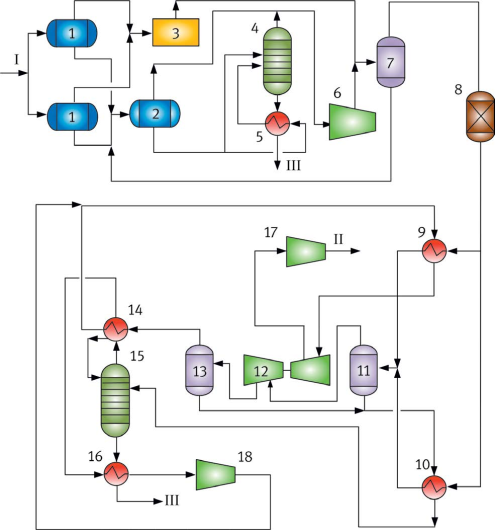
\includegraphics[width=0.8\textwidth]{assets/305}
	\caption*{}
\end{figure}

{\bfseries Рис. 1 - Технологическая схема установки комплексной подготовки
природного газа с глубоким извлечением углеводородов
С\textsubscript{3+}}

I -- нестабильный газовый конденсат; II -- товарный осушенный газ; III
-- деэтанизированный газовый конденсат в блок насосной внешнего
транспорта

𝑀\textsubscript{сырье}=𝑀\textsubscript{газ}+𝑀\textsubscript{СНГ}+𝑀\textsubscript{СУГ}+𝑀\textsubscript{конденсат}+𝑀\textsubscript{потери}

где \emph{M}\textsubscript{сырье} - масса исходного сырья,
𝑀\textsubscript{газ} - масса товарного газа, 𝑀\textsubscript{СНГ}- масса
сжиженного нефтяного газа, \emph{M}\textsubscript{СУГ}- масса сжиженного
углеводородного газа, \emph{M}\textsubscript{конденсат} - масса
конденсата, \emph{M}\textsubscript{потери}- масса потерь.

Расчет количества товарного газа:

𝑀\textsubscript{газ}=𝑀\textsubscript{сырье}·𝐾\textsubscript{газ}

\hspace{0pt}где \emph{K}\textsubscript{газ} - коэффициент извлечения
товарного газа.

Расчет количества сжиженного нефтяного газа:

𝑀\textsubscript{СНГ}=𝑀\textsubscript{сырье}·𝐾\textsubscript{СНГ}

\hspace{0pt}где 𝐾\textsubscript{СНГ} - коэффициент извлечения сжиженного
нефтяного газа.

Расчет количества сжиженного углеводородного газа:

𝑀\textsubscript{СУГ}=𝑀\textsubscript{сырье}·𝐾\textsubscript{СУГ}

\hspace{0pt}где 𝐾\textsubscript{СУГ}- коэффициент извлечения сжиженного
углеводородного газа.

Расчет количества конденсата:

M\textsubscript{конденсат}
=M\textsubscript{сырье}·K\textsubscript{конденсат}

где 𝐾\textsubscript{конденсат}- коэффициент извлечения конденсата.

Пример расчета

Исходные данные:

Состав сырья: метан (70\%), этан (10\%), пропан (8\%), бутан (5\%),
пентан и тяжелее (7\%). Объем сырья: 10000 м³. Коэффициенты извлечения:
товарный газ (85\%), СНГ (5\%), СУГ (7\%), конденсат (3\%).

Расчет:

Масса товарного газа:

𝑀\textsubscript{газ}=10000м\textsuperscript{3}·0.85=8500м\textsuperscript{3}

Масса сжиженного нефтяного газа:

𝑀\textsubscript{СНГ}=10000м\textsuperscript{3}·0.05=500м\textsuperscript{3}

Масса сжиженного углеводородного газа:

M\textsubscript{СУГ} =10000м\textsuperscript{3}
·0.07=700м\textsuperscript{3}

Масса конденсата:

M\textsubscript{конденсат}=10000м\textsuperscript{3}·0.03=300м\textsuperscript{3}

Таким образом, из 10000 м³ исходного сырья получается 8500 м³ товарного
газа, 500 м³ сжиженного нефтяного газа, 700 м³ сжиженного
углеводородного газа и 300 м³ конденсата.

{\bfseries Результаты и обсуждение.} Этот метод позволяет точно рассчитать
количество получаемых продуктов на основе исходных данных и
коэффициентов извлечения, что важно для планирования и оптимизации
процессов переработки углеводородного сырья. Расчет общего объема смеси
углеводородного сырья \emph{V\textsubscript{СУС}},
тыс.~м\textsuperscript{3}, определяется по следующей формуле:

\(\ \ \ \ \ \ \ \ \ \ \ \ \ \ \ \ \ \ \ \ \ \ \ \ \ \ \ \ V_{СУС} = V_{1} + V_{2} + V_{3} + \ldots + V_{n}\)
(1)

где V\textsubscript{1}, V\textsubscript{2}, V\textsubscript{3}, \ldots,
V\textsubscript{n} -- объемы потоков углеводородного сырья, поступающих
в общую смесь углеводородного сырья, тыс. м\textsuperscript{3}.

Расчет доли i-того потока углеводородного сырья ꞷi, от общего количества
смеси углеводородного сырья определяется, по следующей формуле:

\(\omega_{i} = \frac{V_{i}}{V_{СУС}}\) (2)

Расчет мольной доли \emph{j}-того компонента смеси углеводородного
сырья, \emph{x\textsubscript{j}}, \%~(моль), определяется по следующей
формуле:

\(x_{j} = \sum_{i = 1}^{n}{x_{i}^{j} \times \omega_{i}}\) (3)

где, \(x_{i}^{j}\) -- мольная доля \emph{j}-того компонента,
\emph{i}-того потока углеводородного сырья поступающего в общую смесь
углеводородного сырья, \% (моль). Метод пересчета смеси углеводородного
сырья по составу и определение количества выхода продукции --
\({\ n}_{СУС}^{тг},{\ n}_{СУС}^{СУГ},{\ n}_{СУС}^{конд}\), определяется
по соотношению

\(\left( n_{СУС}^{тг},\ n_{СУС}^{СУГ},\ n_{СУС}^{конд},\ n_{С2}^{СУС},n_{С4}^{СУС},n_{С5}^{СУС},n_{С6}^{СУС},\ldots,n_{СО2}^{СУС},n_{N2}^{СУС},\ldots\  \right)\  = \overrightarrow{\Omega_{0}}{\times A}^{- 1}\)
(4)

где, А -- является матрицей от состава \(\overrightarrow{\Omega_{пг}}\),
\(\overrightarrow{\Omega_{суг}}\), \(\overrightarrow{\Omega_{конд}}\):

\(A = \left\| \begin{array}{r}
\begin{array}{r}
\begin{array}{r}
\begin{array}{r}
\overrightarrow{\Omega_{пг}} \\
\overrightarrow{\Omega_{суг}}
\end{array} \\
\overrightarrow{\Omega_{конд}} \\
0\ 1\ 0\ 0\ 0\ 0\ 0\ 0\ 0\ 0\ldots 0 \\
0\ 0\ 0\ 1\ 0\ 0\ 0\ 0\ 0\ 0\ldots 0 \\
0\ 0\ 0\ 0\ 0\ 1\ 0\ 0\ 0\ 0\ldots 0 \\
0\ 0\ 0\ 0\ 0\ 0\ 1\ 0\ 0\ 0\ldots 0 \\
0\ 0\ 0\ 0\ 0\ 0\ 0\ 1\ 0\ 0\ldots 0 \\
0\ 0\ 0\ 0\ 0\ 0\ 0\ 0\ 1\ 0\ldots 0
\end{array} \\
0\ 0\ 0\ 0\ 0\ 0\ 0\ 0\ 0\ 1\ldots 0 \\
\ldots
\end{array} \\
0\ 0\ 0\ 0\ 0\ 0\ 0\ 0\ 0\ 0\ldots 1
\end{array} \right\|\) (5)

Разница между количеством углеводородного вещества в установках и
технологических трубопроводах в начале и в конце расчетного
периода,\(\ \mathrm{\Delta}\overrightarrow{Ν_{запас}}\), определяется
как:

\(\mathrm{\Delta}\overrightarrow{Ν_{запас}}\) =
\(\left( 0,0,0,n_{С2}^{СУС},n_{С4}^{СУС},n_{С5}^{СУС},n_{С6}^{СУС},\ldots,n_{СО2}^{СУС},n_{N2}^{СУС},\ldots \right)\)
(6)

Выражение А\textsuperscript{-1} является обозначением обратной матрицы,
определяется на основе автоматизированных методов или в соответствии
{[}11{]} осуществляется по формуле:

\(A^{- 1} = \frac{1}{|A|} \times S^{T}\) (7)

Где \(|A|\) -- определитель матрицы \emph{A};

\emph{S\textsuperscript{T}} -- транспонированная матрица
(\textbar{}\emph{A\textsubscript{ij}}\textbar)\textsubscript{~i=1\ldots n,
j=1\ldots n};

\emph{A\textsubscript{ij}} -- Алгебраическое дополнение к элементу
матрицы \emph{A} с координатами \emph{(i; j)}, определяемая по схеме:

\begin{itemize}
\item
  вычёркиваем из исходной матрицы \emph{A} i-строчку и j-й столбец.
\item
  получим новую квадратную матрицу, и её умножаем этот на
  (-1)\textsuperscript{i+j}.
\end{itemize}

Определитель матрицы рассчитывается по {[}12{]}.

Расчет (норматива) удельного количества продуктов переработки по
формулам:

\(k_{тг}\  = \ \frac{n_{тг}}{n_{СУС}^{тг}} + \frac{n_{тг} \times \left| \mathrm{\Delta}\overrightarrow{Ν_{запас}} \right|}{n_{СУС}}\)
(8)

\(k_{суг}\  = \ \frac{n_{СУГ}}{n_{СУС}^{СУГ}} + \frac{n_{СУГ} \times \left| \mathrm{\Delta}\overrightarrow{Ν_{запас}} \right|}{n_{СУС}}\)
(9)

\(\ \ \ \ \ \ \ \ \ \ \ \ \ \ \ \ \ \ \ \ \ \ \ \ \ \ \ \ \ \ \ \ k_{конд}\  = \ \frac{n_{конд}}{n_{СУС}^{конд}} + \frac{n_{конд} \times \left| \mathrm{\Delta}\overrightarrow{Ν_{запас}} \right|}{n_{СУС}}\)
(10)

где \emph{n\textsubscript{СУС}}~--~общее количество вещества
углеводородного сырья, поступающего на переработку, кмоль;

\(n_{СУС}^{тг}\) --~количество вещества переработанного товарного газа,
кмоль, рассчитанный на основе состава углеводородного сырья и товарного
газа в соответствии с п. 2;

\(n_{СУС}^{СУГ}\) --~количество вещества, переработанного сжиженного
углеводородного газа, кмоль, рассчитанный на основе состава
углеводородного сырья и сжиженного углеводородного газа в соответствии с
п. 2;

\(n_{СУС}^{конд}\) --~количество вещества переработанного конденсата,
кмоль, рассчитанный на основе состава углеводородного сырья и конденсата
в соответствии с п. 2;

\emph{n}\textsubscript{тг}~--~количество вещества переработанного
товарного газа, кмоль;

\emph{n}\textsubscript{СУГ}~--~количество вещества, переработанного
сжиженного углеводородного газа, кмоль;

\emph{n}\textsubscript{конд}~--~количество вещества вырабатываемого
конденсата, кмоль;

\(\mathrm{\Delta}\overrightarrow{Ν_{запас}}\) -- разница между
количеством углеводородного вещества в установках и технологических
трубопроводах в начале и в конце расчетного периода, определяемый в
соответствии п. 2.

Для определения количества выхода углеводородной продукции, входящего в
состав смеси углеводородного сырья, поступающий на переработку,
применяется следующая формула:

\(V_{тг}^{вых}\  = 24,04012 \times n_{тг}{\times k}_{тг}\),
ст.м\textsuperscript{3} (11)

\(\ \ \ \ \ \ \ \ \ \ \ \ \ \ \ \ \ \ \ \ \ \ \ \ m_{СУГ}^{вых}\  = n_{СУГ}{\times k}_{СУГ} \times M_{СУГ}\),
кг (12)

\(m_{конд}^{вых}\  = n_{конд}{\times k}_{конд} \times M_{конд}\), кг,
(13)

где \emph{n\textsubscript{ТГ}} -- количество вещества переработанного
товарного газа, кмоль, рассчитанный на основе состава смеси
углеводородного сырья и товарного газа в соответствии с Разделом 3;

\emph{n\textsubscript{СУГ}} -- количество вещества, переработанного
сжиженного углеводородного газа, кмоль, рассчитанный на основе состава
смеси углеводородного сырья и сжиженного углеводородного газа в
соответствии с Разделом 3;

\emph{n\textsubscript{конд}} -- количество вещества переработанного
конденсата, кмоль, рассчитанный на основе состава смеси углеводородного
сырья и конденсата в соответствии с Разделом~3;

\emph{k}\textsubscript{тг} \emph{--} удельная норма выхода
переработанного товарного газа;

\emph{k}\textsubscript{СУГ} \emph{--} удельная норма выхода
переработанного сжиженного углеводородного газа;

\emph{k}\textsubscript{конд} \emph{--} удельная норма выхода
переработанного конденсата;

\emph{М}\textsubscript{СУГ} \emph{--} мольная масса переработанного
сжиженного углеводородного газа, кг/кмоль;

\emph{М}\textsubscript{конд} \emph{--} мольная масса переработанного
конденсата, кг/кмоль.

{\bfseries Контроль точности расчета}

Расширенная неопределённость результатов расчета выхода углеводородного
сырья, тыс.~м\textsuperscript{3}, определяется по формуле:

\(\ \ \ \ \ \ \ \ \ \ \ \ \ \ \ \ \ \ \ \ \ \ \ \ \ \ \ \ \ \ \ \ \ \ \ \ \ \ \ \ \ \ \ \ \ \ U = k \bullet u_{l}\)
(14)

где \emph{l} -- коэффициент охвата, принимает значение в интервале 2-3,
что соответствует выбранному уровню доверия 95-99 \%;

\emph{u\textsubscript{k}} -- стандартная неопределённость,
тыс.~м\textsuperscript{3}, определяемая по формуле:

\(u_{k} = \sum_{i = 0}^{n}{V_{i} \bullet \mathrm{\Delta}\Omega_{i}} + \sum_{j = 0}^{m}{V_{j} \bullet \delta_{j}}\)
(15)

где \emph{V} -- общий объем смеси углеводородного сырья, поступающий на
переработку, в расчетный период, тыс.~м\textsuperscript{3};

\emph{ΔΩ\textsubscript{i}} -- установленная погрешность определения
компонентного состава\\
\emph{i}-го анализа;

\emph{V\textsubscript{i}} -- количество газа, соответствующего
компонентному составу полученному \emph{i}-ым анализом, в расчетный
период, тыс.~м\textsuperscript{3}, участвующим в учете газа в системе
переработки углеводородного сырья;

\emph{δ\textsubscript{j}} -- установленная погрешность \emph{j}-го
замерного узла, в соответствии с таблицей Е.1;

\emph{V\textsubscript{j}} -- количество зафиксированного газа
\emph{j}-ым замерным узлом, в расчетный период,
тыс.~м\textsuperscript{3}, участвующим в учете газа в системе
переработки углеводородного сырья.

Контроль правильности результатов расчета:

\(\frac{u_{l}}{V} \times 100 < K_{n}\) (16)

где \emph{V} -- общий объем смеси углеводородного сырья, поступающий на
переработку, в расчетный период, тыс.~м\textsuperscript{3};

\emph{u\textsubscript{l}} -- стандартная неопределённость, определяемая
по формуле (15), тыс.~м\textsuperscript{3};

\emph{K\textsubscript{n}} -- норматив контроля, \%;

\emph{K\textsubscript{n}} принимается не более 1\%.

Для перевода количества вещества в массу смеси углеводородного сырья
применяется следующая формула:

\(m_{СУС}\  = n \times M_{УС}\), кг, (17)

где \emph{n}~--~количество вещества смеси углеводородного сырья, кмоль;

\emph{M\textsubscript{УС}}~--~молярная масса смеси углеводородного
сырья, кг/кмоль.

Для перевода массу в количество вещества смеси углеводородного сырья
применяется следующая формула:

\(n\  = \frac{m_{УС}}{M_{УС}}\), кмоль,

где, \emph{m\textsubscript{УС}}~--~масса смеси углеводородного сырья,
кг;

\emph{M\textsubscript{УС}}~--~молярная масса смеси углеводородного
сырья, кг/кмоль.

Для перевода количества вещества в объем газа в стандартных условиях
смеси углеводородного сырья применяется следующая формула:

\(\ \ \ \ \ \ \ \ \ \ \ \ \ \ \ \ \ \ \ \ \ \ \ \ \ \ \ \ \ V_{ст.у.}\  = 24,04012 \times n\),
м\textsuperscript{3} (18)

где \emph{n} --~количество вещества смеси углеводородного сырья, кмоль.

Для перевода объем газа (в стандартных условиях) в количество вещества
смеси углеводородного сырья применяется следующая формула:

\(n\  = 0,04159713 \times V_{ст.у.}\), кмоль (19)

Где \emph{V\textsubscript{ст.у.}}~--~объем углеводородного газа в
стандартных условиях, м\textsuperscript{3}.

Молярные массы компонентов смеси углеводородного сырья приведены в
таблице А.1.

Плотность газа в стандартных условиях, \emph{ρ},
кг/м\textsuperscript{3}, определяется по формуле:

ρ = 0,04159713⋅М (20)

где \emph{М} -- молярная масса, кг/кмоль.

Экологические и экономические аспекты. Научно-исследовательская работа
по разработке и анализу методов переработки углеводородного сырья
предлагает инновационные решения, которые существенно повышают
экономическую эффективность и снижают экологическую нагрузку.
Использование передовых технологий и точных аналитических методов
позволяет улучшить переработку сырья, снизить затраты и повысить доходы,
одновременно способствуя охране окружающей среды за счет снижения
выбросов и рационального использования ресурсов. Точные методы расчета и
оптимизация технологических процессов позволяют уменьшить объемы
сжигания газа на факелах, что снижает выбросы загрязняющих веществ и
парниковых газов в атмосферу. Внедрение современных технологий
переработки углеводородного сырья способствует снижению экологической
нагрузки и улучшению экологических показателей предприятий. Оптимизация
переработки углеводородного сырья позволяет рационально использовать
ресурсы, минимизируя потери и воздействие на окружающую среду.
Применение энергоэффективных технологий, таких как мембранные,
адсорбционные и абсорбционные процессы, улучшает процессы переработки и
снижает энергозатраты, что благоприятно сказывается на экологии.
Современные методы переработки, такие как низкотемпературная
ректификация и использование высокоэффективных насадок в колоннах,
уменьшают энергозатраты и выбросы, повышая экологическую безопасность
процессов. Методы расчета материального баланса и аналитические
технологии позволяют точно определять количество выходящих продуктов
(товарный газ, сжиженный углеводородный газ, конденсат), что улучшает
планирование и управление ресурсами, повышая рентабельность
производственных процессов. Оптимизация технологических процессов и
использование передовых математических методов позволяют достичь высокой
точности и надежности расчетов, что улучшает планирование и управление
ресурсами. Применение передовых технологий, таких как плазмохимические и
волновые методы, снижает капитальные затраты на переработку
углеводородного сырья, улучшая экономические показатели предприятий.
Разработка методов переработки газа непосредственно на месте его добычи
снижает затраты на транспортировку, что особенно важно для удаленных
месторождений. Внедрение автоматизированных систем расчетов сокращает
время на проведение расчетов и снижает вероятность ошибок, что
дополнительно повышает экономическую эффективность переработки
углеводородного сырья. Продажа единиц сокращения выбросов (ЕСВ) помогает
улучшить экономические показатели проектов и компенсировать часть затрат
на создание инфраструктуры для утилизации попутного нефтяного газа
(ПНГ).

{\bfseries Выводы:} Уникальный разработанный метод предлагает расчет общего
объема смеси углеводородного сырья, а также доли каждого потока сырья в
общей смеси. Это позволяет точно определить мольную долю каждого
компонента в смеси. Применение матричных методов для пересчета состава
углеводородного сырья на выход продукции. Использование обратной матрицы
и компонентного состава позволяет точно определить количество выходящих
продуктов. Методика включает расчет удельного выхода различных продуктов
(товарный газ, сжиженный углеводородный газ, конденсат) на основе общего
количества углеводородного сырья и технологических потерь. Определение
количества выходящей продукции для каждого конкретного потока
углеводородного сырья позволяет детализировать расчет и повысить
точность. Введение показателя расширенной неопределенности и методов
контроля правильности расчетов. Это обеспечивает уверенность в точности
и достоверности результатов. Применение формул для перевода количества
вещества в массу и объем и наоборот. Это позволяет легко конвертировать
результаты расчетов в необходимые единицы измерения.

{\bfseries Литература}

1.Муллахметова Л.И., Черкасова Е.И. Попутный нефтяной газ: подготовка,
транспортировка и переработка// Вестник Казанского технологического
университета.- 2015. - Т.18(19)- С. 83-90

2.Азарова А.И. Инновационные технологии в нефтедобыче и их отражение в
системе управления вертикально интегрированных нефтяных компаний//
Проблемы учёта и финансов.-2012.- № 4 (8) 2012. С.35-47

3.Владимиров А.И. Экология нефтегазового комплекса /А.И. Владимиров. М:
Нефть и газ.- 2003.- 415 с. ISBN 5-7246-0232

4.Муллахметова Л.И., Черкасова Е.И., Сигбатуллина Р.И., Бикмухаметова
Г.К., Мустафина А.М., Салахов И.И. Газофракционирование // Вестник
технологического университета.- 2016.- Т19(24) - С. 49-555.

5.Семенова Т.А. Очистка технологических газов / Т.А. Семенова и др -M.:
Химия- 1997.-314 с.

6.Абдуллин А.И., Солодова Н.Л., Пиролиз углеводородного сырья. Учебное
пособие / Солодова Н.Л., Абдуллин А.И.// КГТУ. - Казань, 2008.- 240 с.
ISBN:~978-5-7882-0518-2

7.Аджиев А.Ю., Пуртов П.А. Подготовка и переработка попутного нефтяного
газа в России: в 2 ч. Ч. 2 / А.Ю.Аджиев, П.А.Пуртов. - Краснодар: ЭДВИ,
2014. - 504 с.

8.Ибрагимова А.В. Методическое обеспечение управления эффективностью
утилизации попутного нефтяного газа на нефтедобывающих предприятиях:
дис. \ldots{} к.э.н. Удмуртский государственный университет. -2015. --
166 с.

9.Муродов М. Н. Системы разработки газоконденсатных месторождений //
Молодой ученый.- 2014.- №1.- С. 102-103.

10.Аристова В.В. Альтернативные комплексные технологии переработки
попутных нефтяных газов/ В.В. Аристова, А.С. Дорофеев
(http://www.gazcompany.ru/gazpngfull.html)

11.Даутов Р.З., Тимербаев М.Р. Численные методы. Решение задач линейной
алгебры и дифференциальных уравнений: учебное пособие. --- Казань:
К(П)ФУ, 2021.-168 с.

12.Кабанова О.А. Вычисление определителя. Нахождение обратной матрицы/
Мет. пособие по курсу «Высшая математика» раздел «Линейная алгебра». М.:
МАИ, 2015. -- 15 с.

{\bfseries References}

1.Mullahmetova L.I., Cherkasova E.I. Poputnyj neftjanoj gaz: podgotovka,
transportirovka i pererabotka// Vestnik Kazanskogo tehnologicheskogo
universiteta.- 2015. - T.18(19)- S. 83-90.

{[}in Russ.{]}

2.Azarova A.I. Innovacionnye tehnologii v neftedobyche i ih otrazhenie v
sisteme upravlenija vertikal\textquotesingle no integrirovannyh
neftjanyh kompanij// Problemy uchjota i finansov.-2012.- № 4 (8) 2012.
S.35-47. {[}in Russ.{]}

3.Vladimirov A.I. Jekologija neftegazovogo kompleksa /A.I. Vladimirov.
M: Neft\textquotesingle{} i gaz.- 2003.- 415 s. ISBN 5-7246-0232. {[}in
Russ.{]}

4.Mullahmetova L.I., Cherkasova E.I., Sigbatullina R.I., Bikmuhametova
G.K., Mustafina A.M., Salahov I.I. Gazofrakcionirovanie // Vestnik
tehnologicheskogo universiteta.- 2016.- T19(24) - S. 49-555. {[}in
Russ.{]}

5.Semenova T.A. Ochistka tehnologicheskih gazov / T.A. Semenova i dr
-M.: Himija- 1997.-314 s.

6.Abdullin A.I., Solodova N.L., Piroliz uglevodorodnogo
syr\textquotesingle ja. Uchebnoe posobie / Solodova N.L., Abdullin
A.I.// KGTU. - Kazan\textquotesingle, 2008.- 240 s. ISBN:
978-5-7882-0518-2. {[}in Russ.{]}

7.Adzhiev A.Ju., Purtov P.A. Podgotovka i pererabotka poputnogo
neftjanogo gaza v Rossii: v 2 ch. Ch. 2 / A.Ju.Adzhiev, P.A.Purtov. -
Krasnodar: JeDVI, 2014. - 504 s. {[}in Russ.{]}

8.Ibragimova A.V. Metodicheskoe obespechenie upravlenija
jeffektivnost\textquotesingle ju utilizacii poputnogo neftjanogo gaza na
neftedobyvajushhih predprijatijah: dis. \ldots{} k.je.n. Udmurtskij
gosudarstvennyj universitet. -2015. -- 166 s. {[}in Russ.{]}

9.Murodov M. N. Sistemy razrabotki gazokondensatnyh mestorozhdenij //
Molodoj uchenyj.- 2014.- № 1.- S. 102-103. {[}in Russ.{]}

10.Aristova V.V. Al\textquotesingle ternativnye kompleksnye tehnologii
pererabotki poputnyh neftjanyh gazov/ V.V. Aristova, A.S. Dorofeev
(http://www.gazcompany.ru/gazpngfull.html). {[}in Russ.{]}

11.Dautov R.Z., Timerbaev M.R. Chislennye metody. Reshenie zadach
linejnoj algebry i differencial\textquotesingle nyh uravnenij: uchebnoe
posobie. --- Kazan\textquotesingle: K(P)FU, 2021.-168 s. {[}in Russ.{]}

12.Kabanova O.A. Vychislenie opredelitelja. Nahozhdenie obratnoj
matricy/ Met. posobie po kursu «Vysshaja matematika» razdel «Linejnaja
algebra». M.: MAI, 2015.- 15 s. {[}in Russ.{]}

\emph{{\bfseries Сведения об авторах}}

Сейлханов К.К. - магистр математики, директор Товарищество с
ограниченной ответственностью «ГЦПК «Кəсіпкер», Астана, Казахстан,
e-mail: kks\_kz@mail.ru;Мурзагалиев Б.Т. - магистр по специальности
«Химическая технология взрывчатых веществ и пиротехнических средств»,
технический Директор Товарищество с ограниченной ответственностью

«ГЦПК «Кəсіпкер, Астана, Казахстан, e-mail:
murzagaliyev.b.t@gmail.com;Даулетжанова Ж.Т. - доктор PhD,
преподаватель, Казахский университет технологии и бизнеса им.
К.Кулажанова, Астана, Казахстан, e-mail: kaliyeva\_zhanna@mail.ru;

Сейлханова М.Т. - магистр педагогических наук, научный сотрудник
Товарищество с ограниченной ответственностью «ГЦПК «Кəсіпкер», Астана,
Казахстан, e-mail: mbt\_kz@mail.ru;

Бахтияр С. - магистр педагогических наук начальник отдела
Нормативно-технической документации Товарищество с ограниченной
ответственностью «ГЦПК «Кəсіпкер»,Астана, Казахстан, e-mail:
serik19.98.01@gmail.com

\emph{{\bfseries Information about authors}}

Seilkhanov K.K.- Director of Limited liability partnership «ГЦПК
«Кəсіпкер», Astana, Kazakhstan, Master of Mathematics, e-mail:
kks\_kz@mail.ru;

Murzagaliev B.T. - Technical Director of Limited liability partnership
«ГЦПК «Кəсіпкер», Astana, Kazakhstan, Master\textquotesingle s degree in
"Chemical technology of explosives and pyrotechnics", e-mail:
murzagaliyev.b.t@gmail.com;

Dauletzhanova Zh.T. - PhD, Lecturer, Kazakh University of Technology and
Business, Astana, Kazakhstan, e-mail: kaliyeva\_zhanna@mail.ru;

Seilkhanova M.T. - Researcher of Limited liability partnership «ГЦПК
«Кəсіпкер»,Astana, Kazakhstan, Master of Educational Sciences, e-mail:
mbt\_kz@mail.ru;

Bakhtiyar S. - Head of the Regulatory and Technical Documentation
Department in Limited liability partnership «ГЦПК «Кəсіпкер», Astana,
Kazakhstan, Master of Educational Sciences, e-mail:
serik19.98.01@gmail.com